\section{Коэффициент усиления}
\subsection{Система 1}
Рассмотрим объект, заданный передаточной функцией:
\begin{eqnarray}
    W_1(s) = \frac{K(s - 9)}{s^2 + s + 8}
\end{eqnarray}

Посмотрим годограф Найквиста для этой системы при различных значениях коэффициента усиления $K$ (см. рис. \ref{fig:task4_nyquist}).
\begin{figure}[ht!]
    \begin{subfigure}{0.5\textwidth}
        \centering
        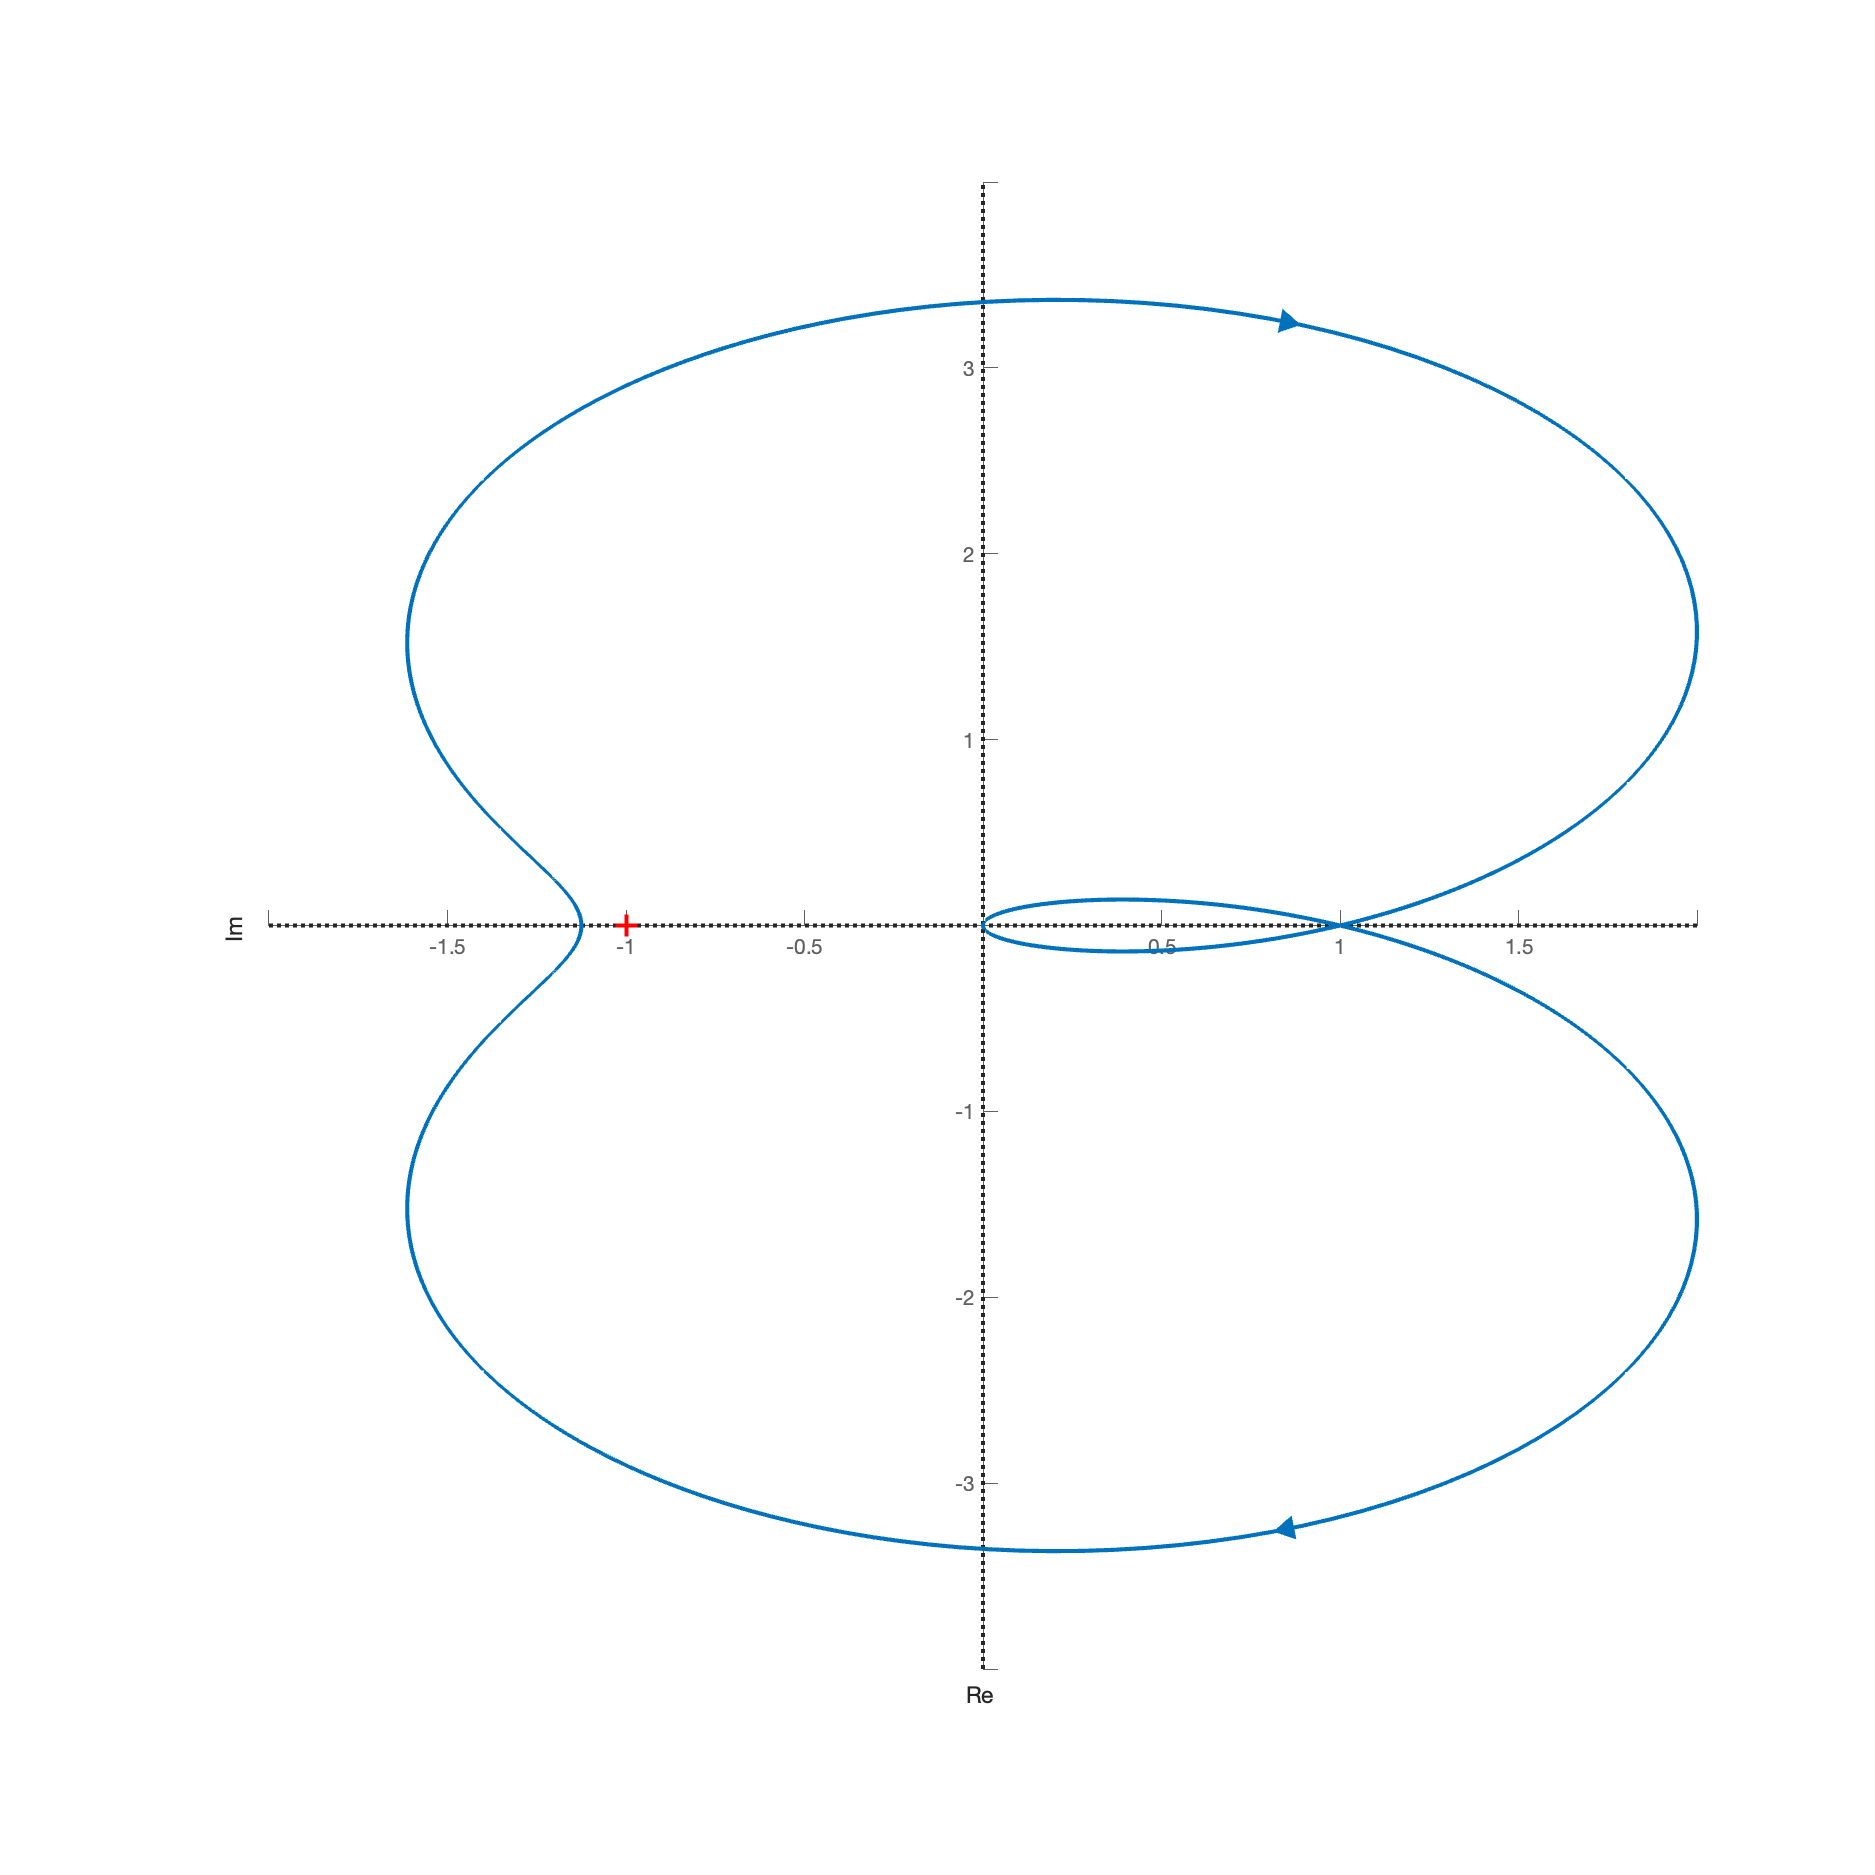
\includegraphics[width=\textwidth]{media/plots/task4_nyquist_1.png}
        \caption{$K = 1$}
    \end{subfigure}%
    \begin{subfigure}{0.5\textwidth}
        \centering
        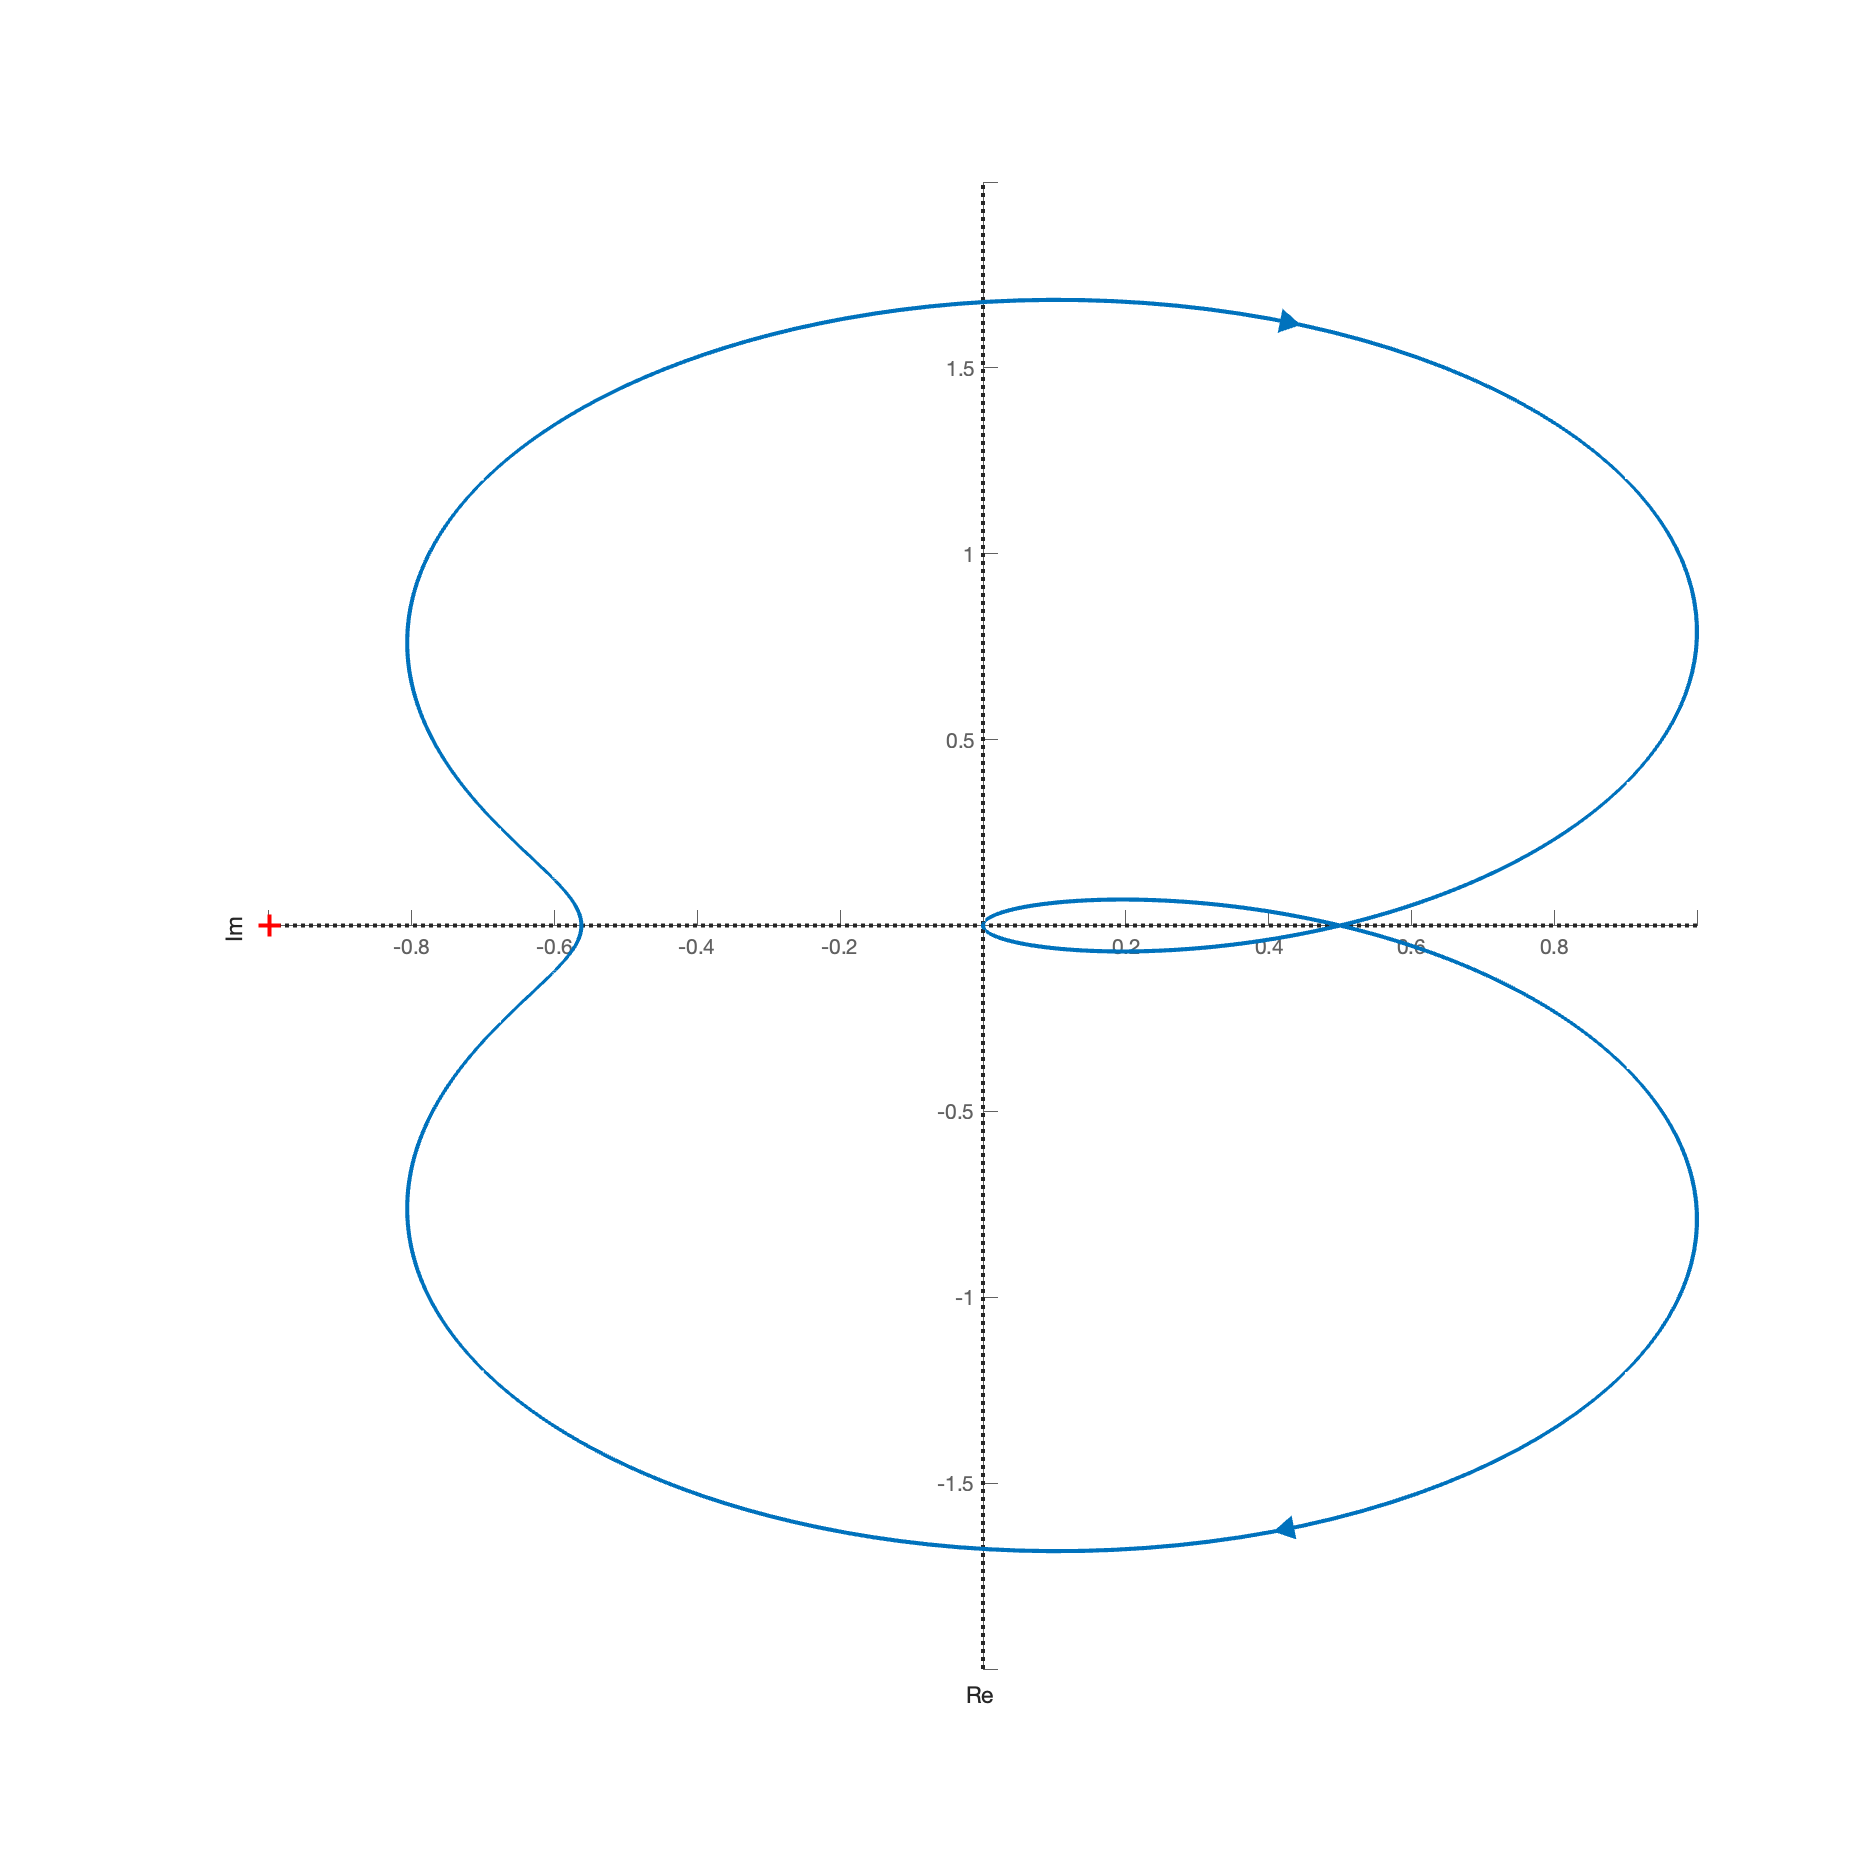
\includegraphics[width=\textwidth]{media/plots/task4_nyquist_2.png}
        \caption{$K = 0.5$}
    \end{subfigure}
    \begin{subfigure}{0.5\textwidth}
        \centering
        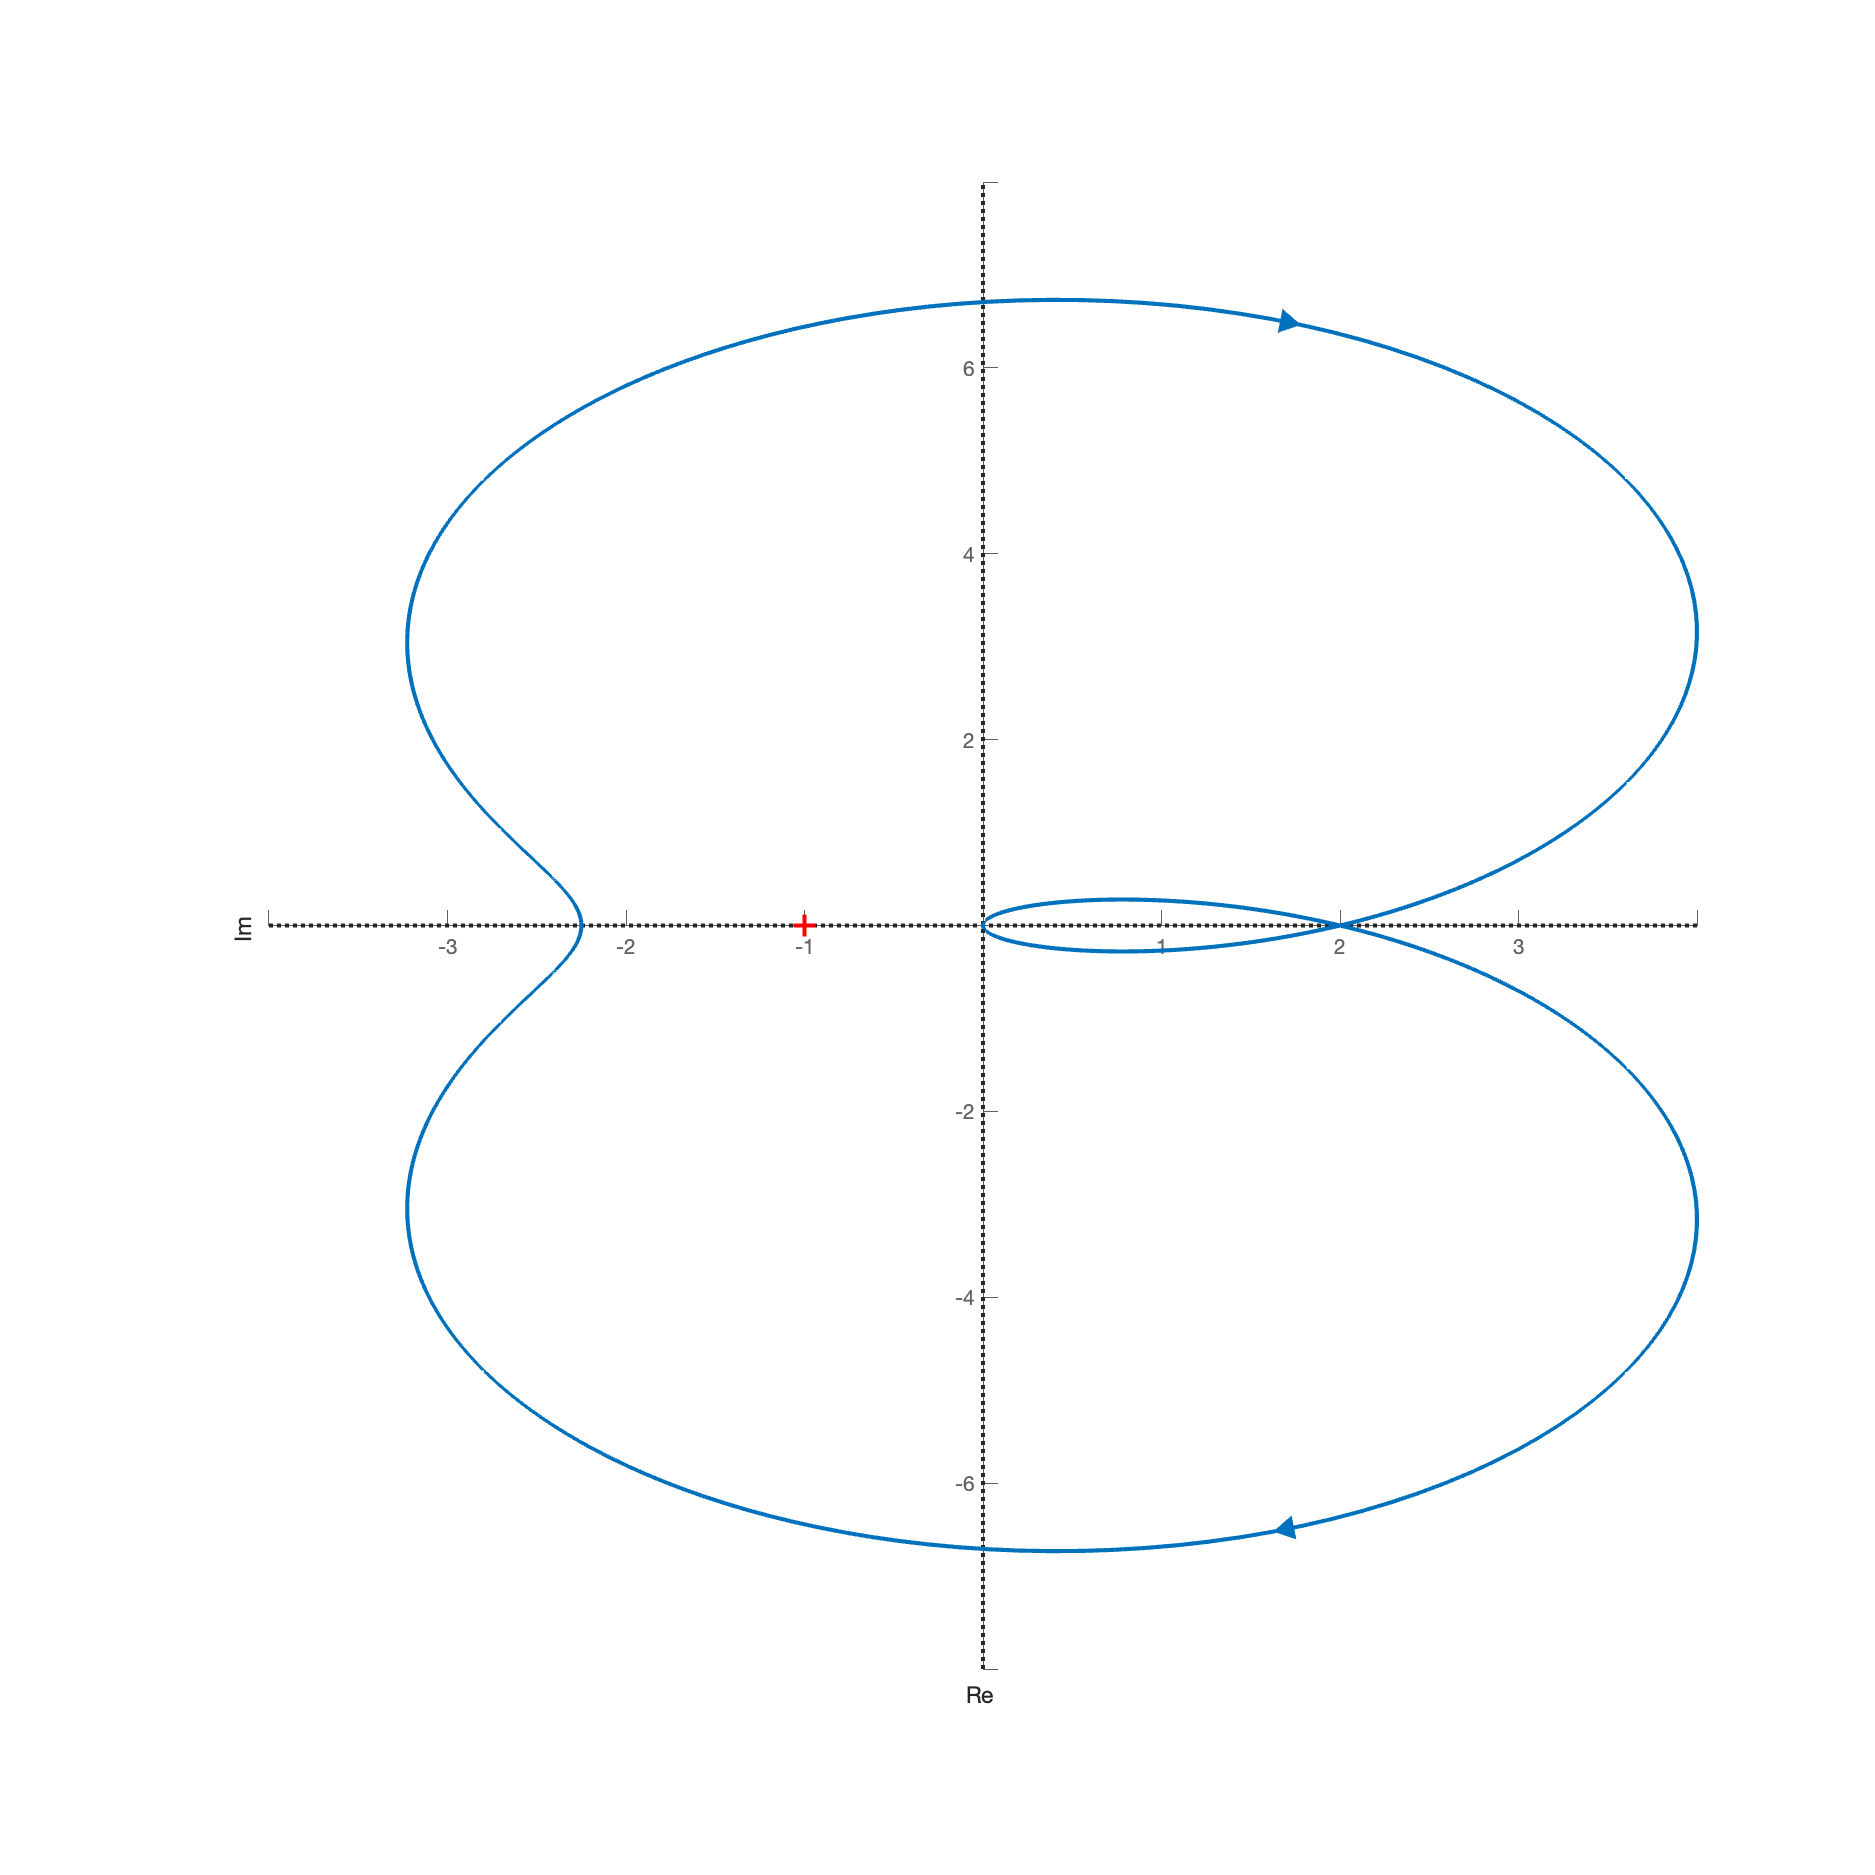
\includegraphics[width=\textwidth]{media/plots/task4_nyquist_3.png}
        \caption{$K = 2$}%
    \end{subfigure}
    \begin{subfigure}{0.5\textwidth}
        \centering
        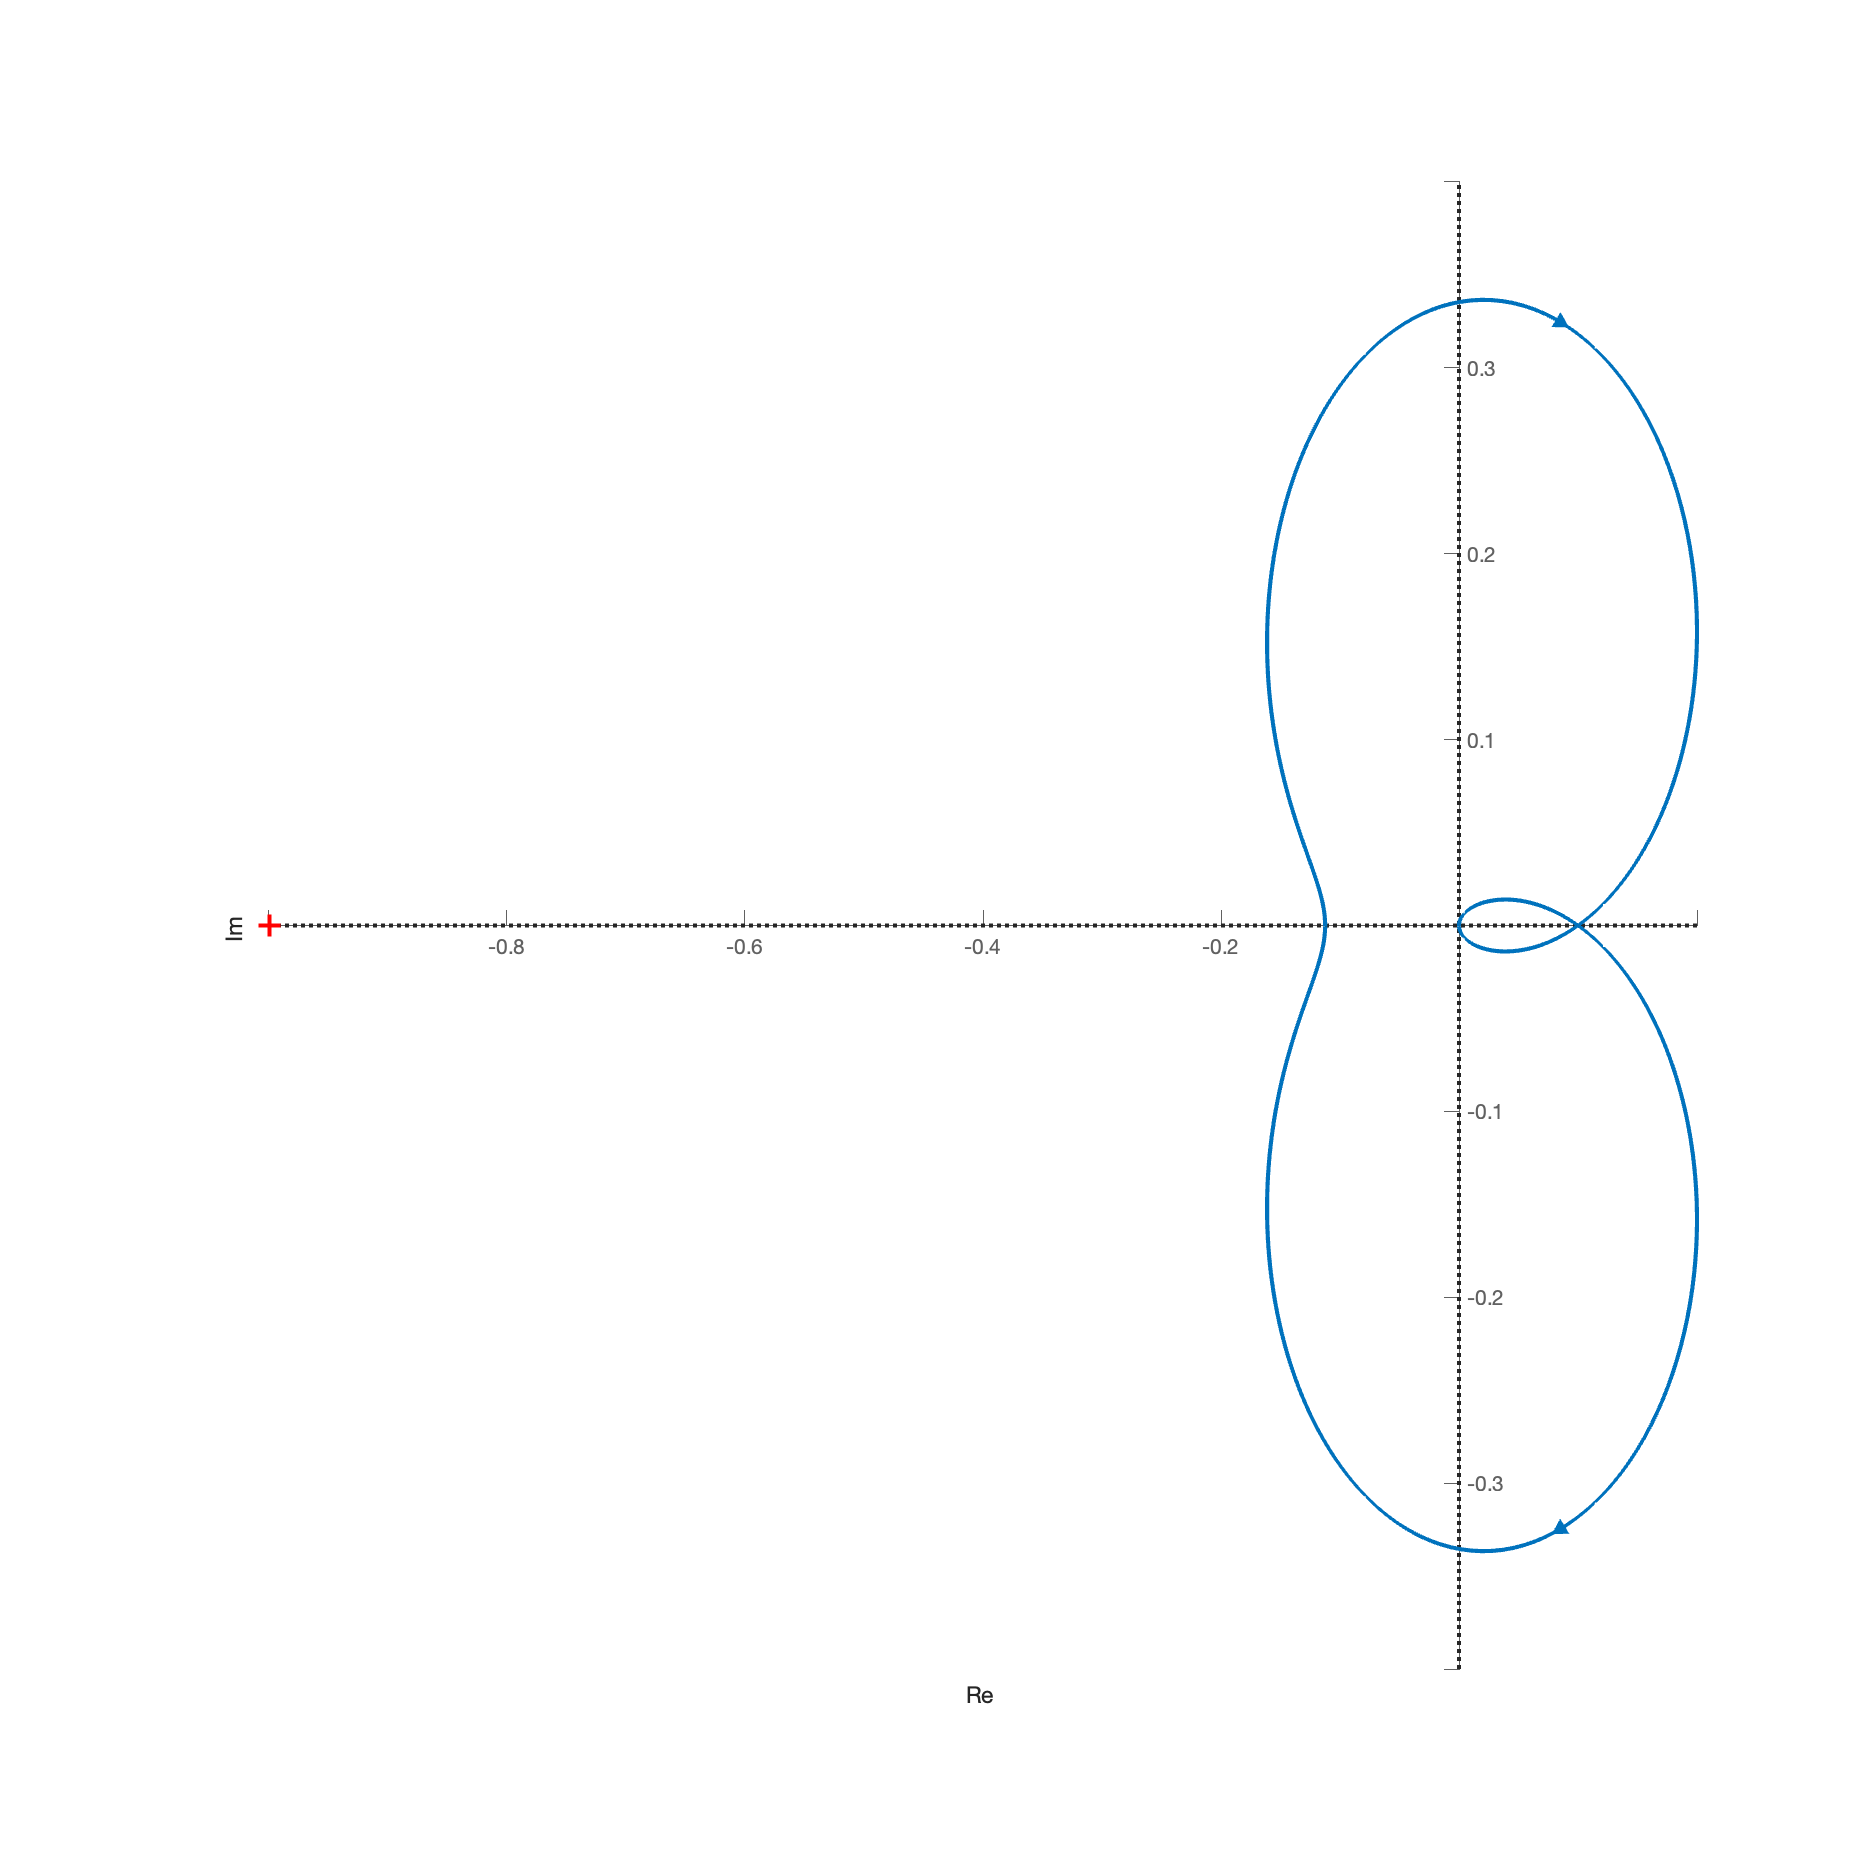
\includegraphics[width=\textwidth]{media/plots/task4_nyquist_4.png}
        \caption{$K = 0.1$}
    \end{subfigure}
    \caption{Годограф Найквиста для различных значений коэффициента усиления $K$}
    \label{fig:task4_nyquist}
\end{figure}

Видно, что при увеличении $K$ годограф \textit{растягивается} по горизонтали и вертикали, в какой-то момент задевая точку $(-1, 0)$. 
Отсюда можно сделать вывод, что значение коэффициента усиления $K$ влияет на устойчивость системы.

Разомкнутая система имеет полюса: 
\begin{equation}
    s_{1,2} = -\frac{1}{2} \pm \frac{\sqrt{31}}{2}i
\end{equation}
Таким образом, разомкнутая система является устойчивой.

Найдем передаточную функцию замкнутой системы:
\begin{eqnarray}
    W_{1c}(s) = \frac{K(s - 9)}{s^2 + s + 8 + K(s - 9)} = \frac{K(s - 9)}{s^2 + (1 + K)s + 8 - 9K}
\end{eqnarray}
Найдем полюса замкнутой системы:
\begin{equation}
    \begin{array}{ll}
        s^2 + (1 + K)s + 8 - 9K = 0 \\
        s_{1, 2} = \frac{-(1 + K) \pm \sqrt{(1 + K)^2 - 4(8 - 9K)}}{2}
    \end{array}
\end{equation}
При $(1 + K)^2 - 4(8 - 9K) <= 0$ в системе будут только устойчивые полюса, рассмотрим обратный случай:
Данная система может иметь только один неустойчивый полюс: 
\begin{equation}
    \begin{array}{ll}
        (1 + K)^2 - 4(8 - 9K) > 0 \\ 
        (1 + K) < \sqrt{(1 + K)^2 - 4(8 - 9K)} \\
        (1 + K)^2 < (1 + K)^2 - 4(8 - 9K) \\
        (8 - 9K) < 0 \\
        \Rightarrow K \in \left(\frac{8}{9}, +\infty\right)
    \end{array}
\end{equation}
Так как по условию $K > 0$, то замкнутая система будет устойчивой при $K \in \left(0, \frac{8}{9}\right)$.

Для нахождения запаса устойчивости по амплитуде построим АФЧХ замкнутой системы при $K = 1$ (см. рис. \ref{fig:task4_freqs}).
\begin{figure}[ht!]
    \centering
    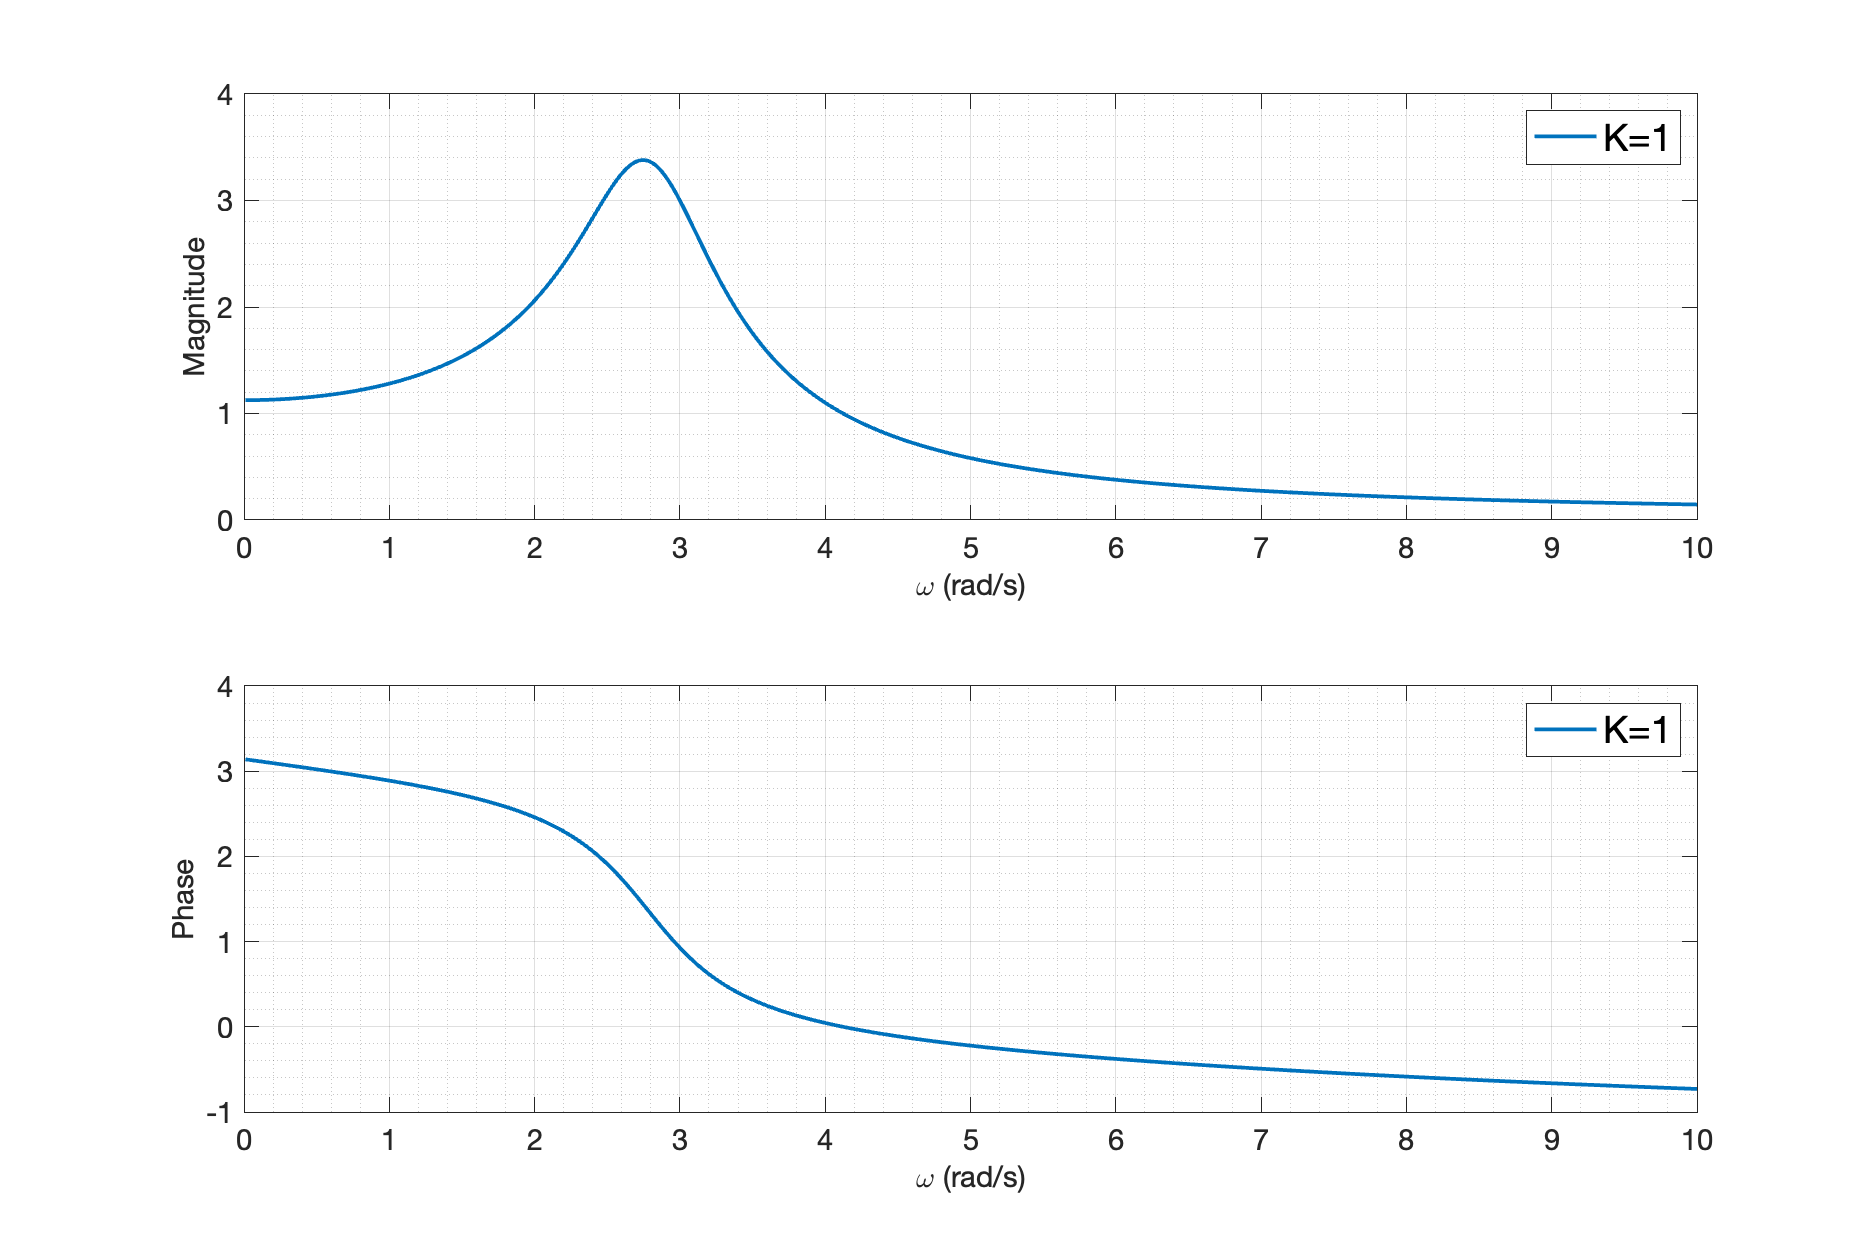
\includegraphics[width=\textwidth]{media/plots/task4_freqs.png}
    \caption{АФЧХ замкнутой системы при $K = 1$}
    \label{fig:task4_freqs}
\end{figure}

График ФЧХ пересекает критический отрезок $3\pi$ при частоте $\omega_c  = 0.55$, при этом 
амплитуда при этой частоте равна $1.125$. Таким образом, \textit{запас} устойчивости по амплитуде равен 
\begin{equation}
    A_c = \frac{1}{A(\omega_c)} = \frac{1}{1.125} = \frac{8}{9}
\end{equation}
что равно критическому значению коэффициента усиления. Так как полученное значение меньше 
единицы, запаса устойчивости нет. 

Проведем моделирование замкнутой системы при различных значениях коэффициента усиления $K$ (см. рис. \ref{fig:task4_step} и \ref{fig:task4_impulse}).
\begin{figure}[ht!]
    \begin{subfigure}{0.5\textwidth}
        \centering
        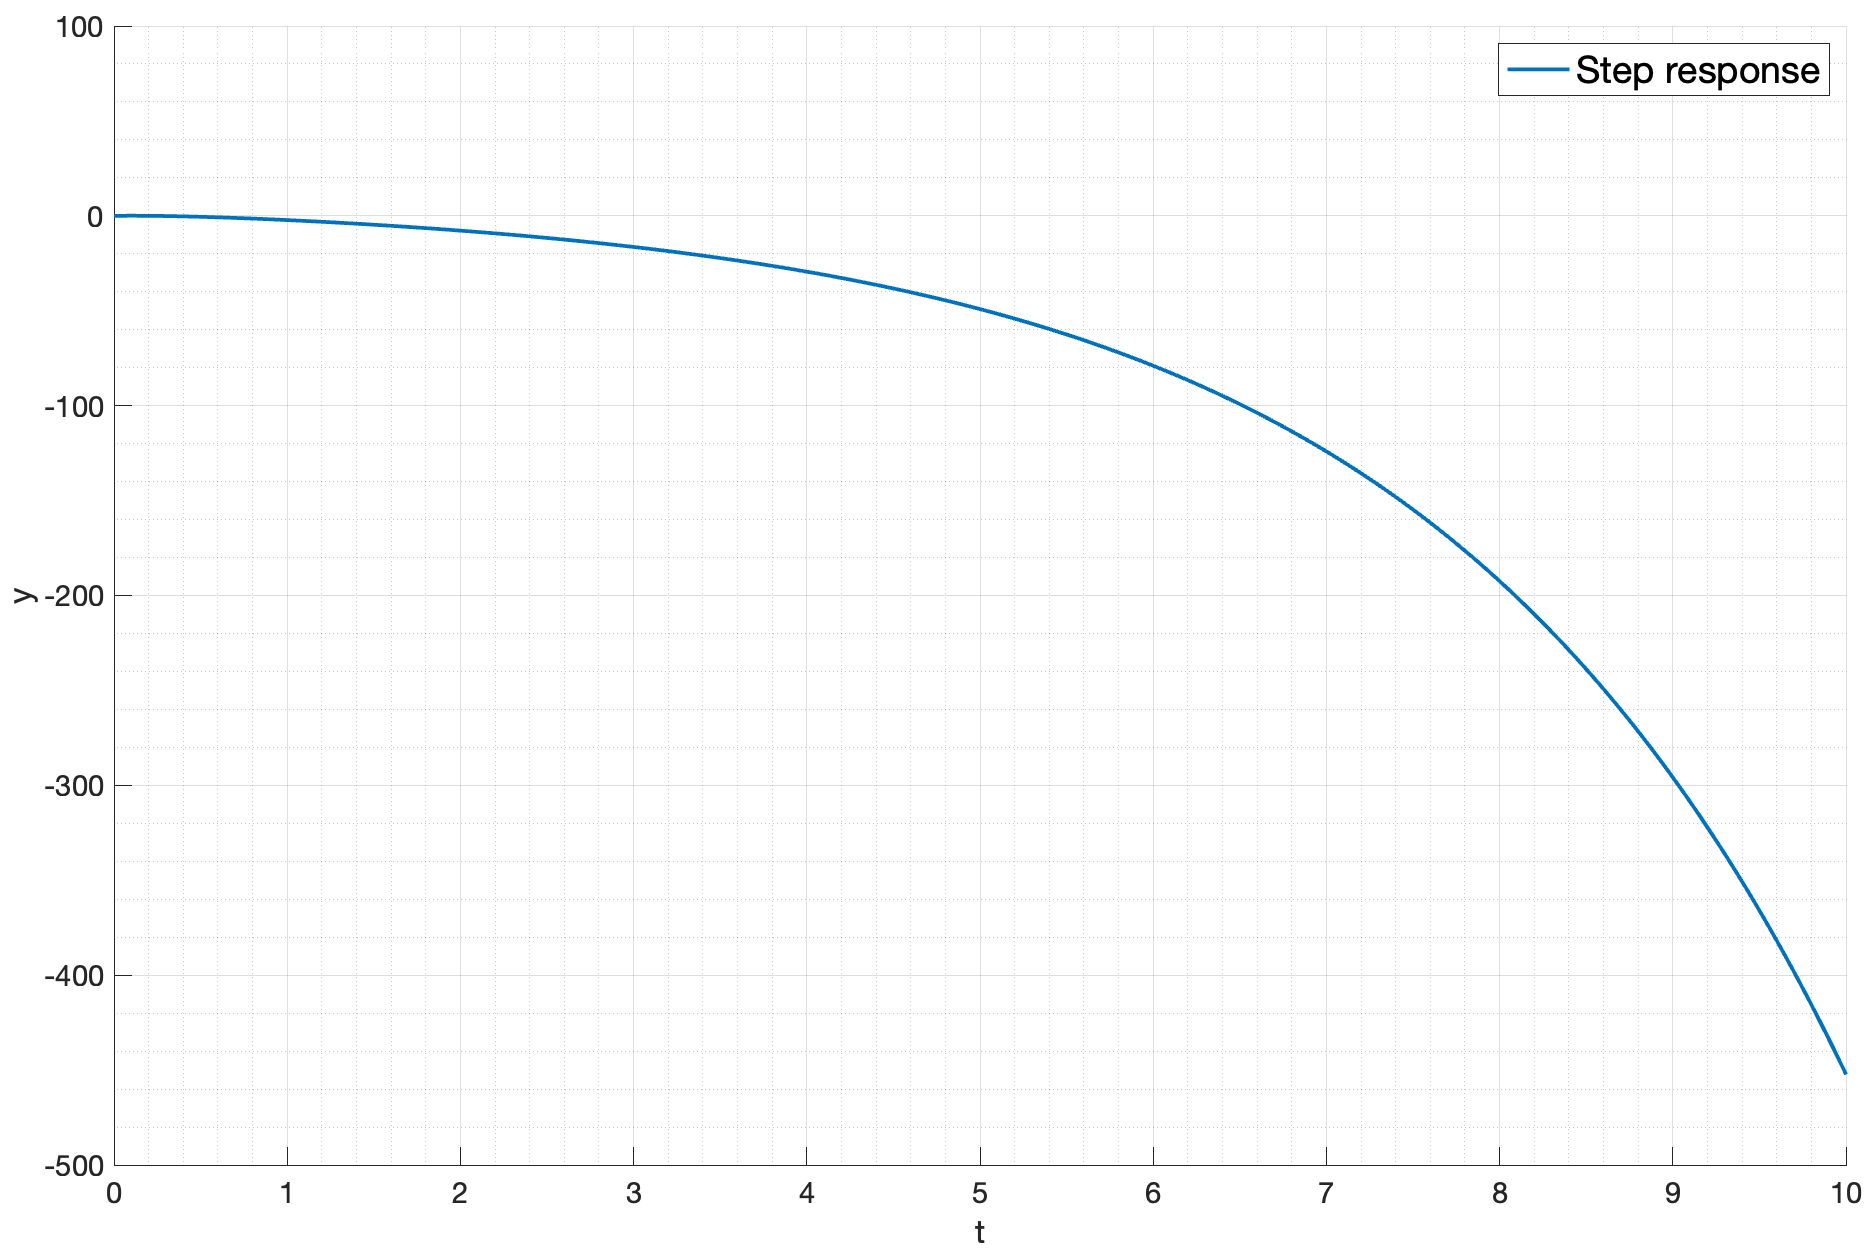
\includegraphics[width=\textwidth]{media/plots/task4_step_response_closed_1.png}
        \caption{$K = 1$}
    \end{subfigure}%
    \begin{subfigure}{0.5\textwidth}
        \centering
        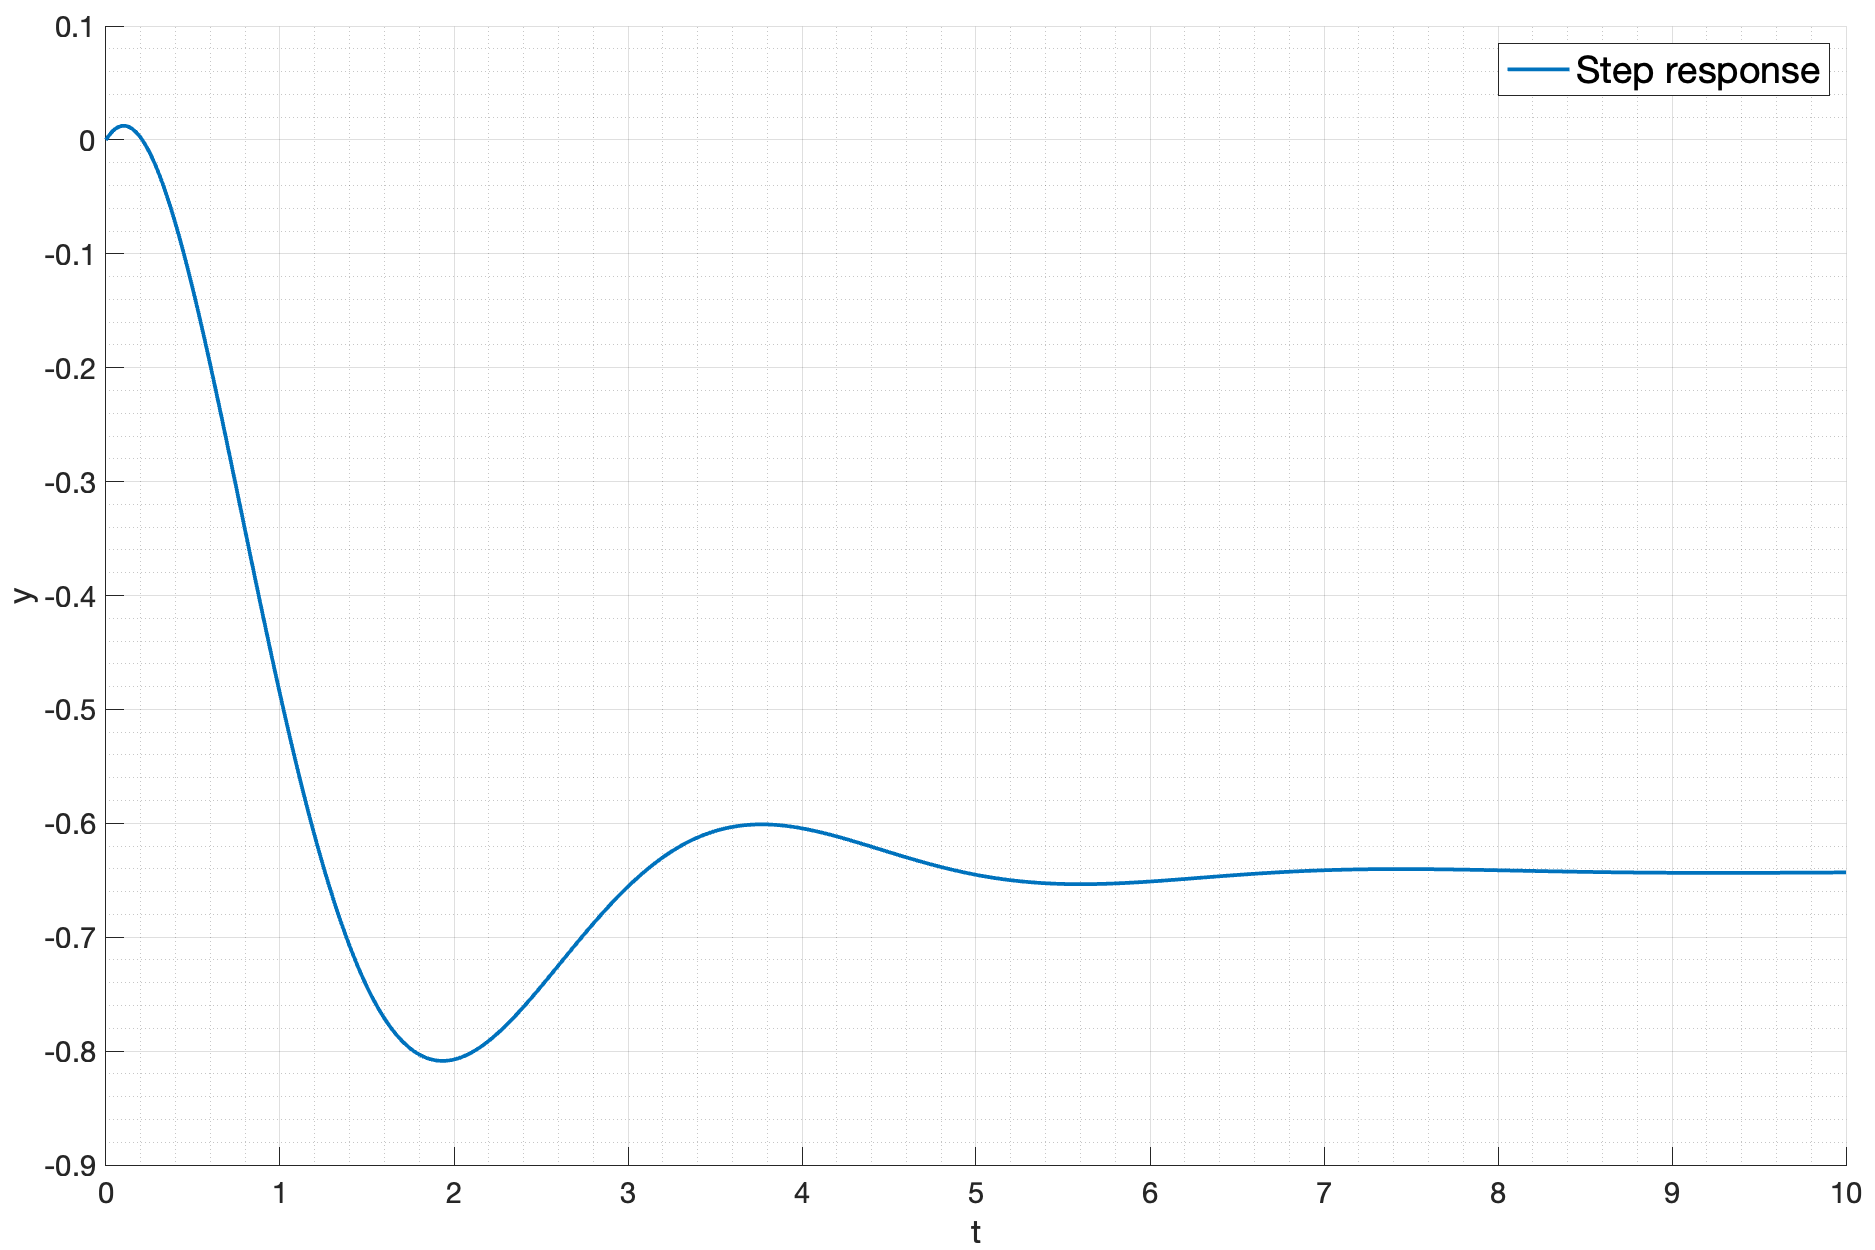
\includegraphics[width=\textwidth]{media/plots/task4_step_response_closed_2.png}
        \caption{$K = 0.5$}
    \end{subfigure}
    \begin{subfigure}{0.5\textwidth}
        \centering
        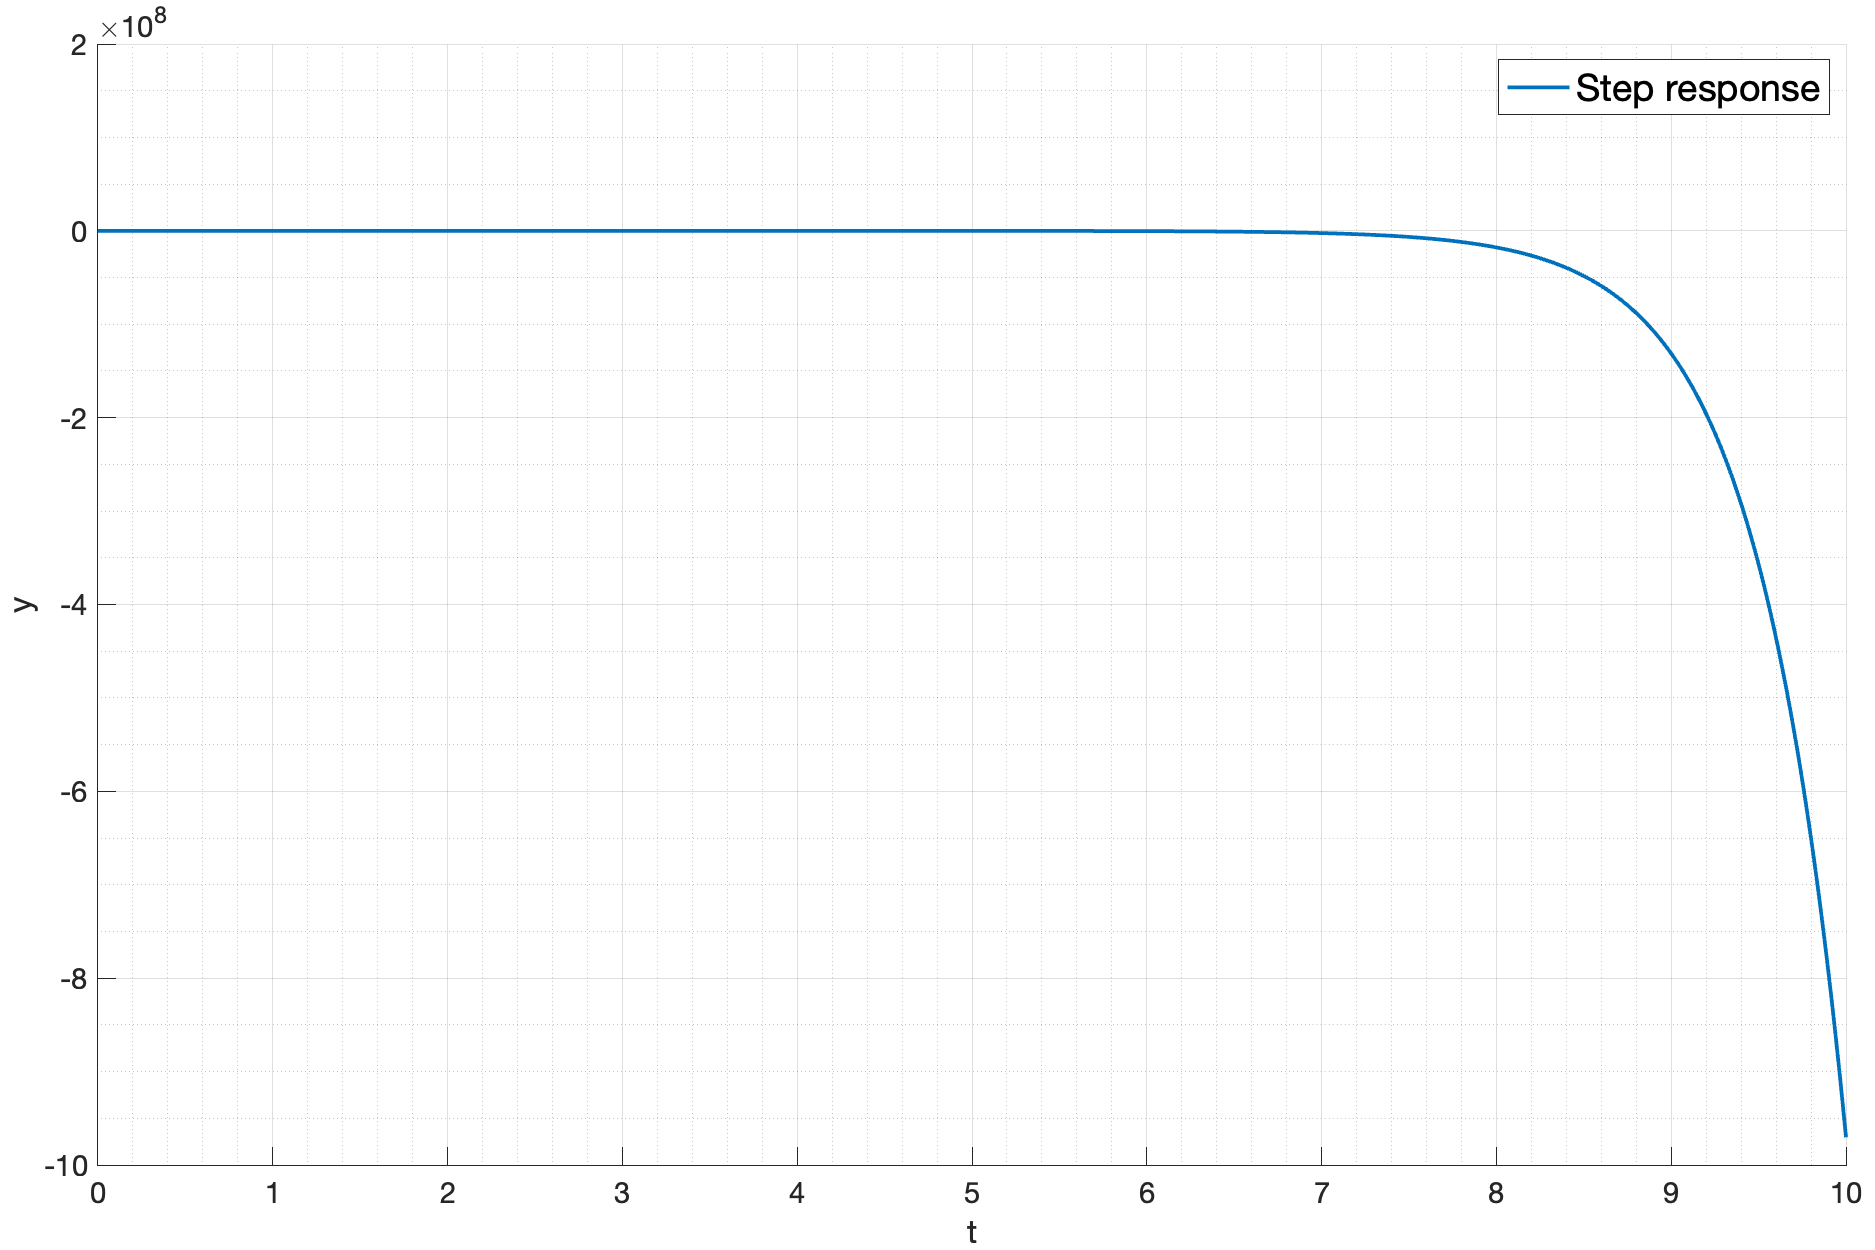
\includegraphics[width=\textwidth]{media/plots/task4_step_response_closed_3.png}
        \caption{$K = 2$}
    \end{subfigure}%
    \begin{subfigure}{0.5\textwidth}
        \centering
        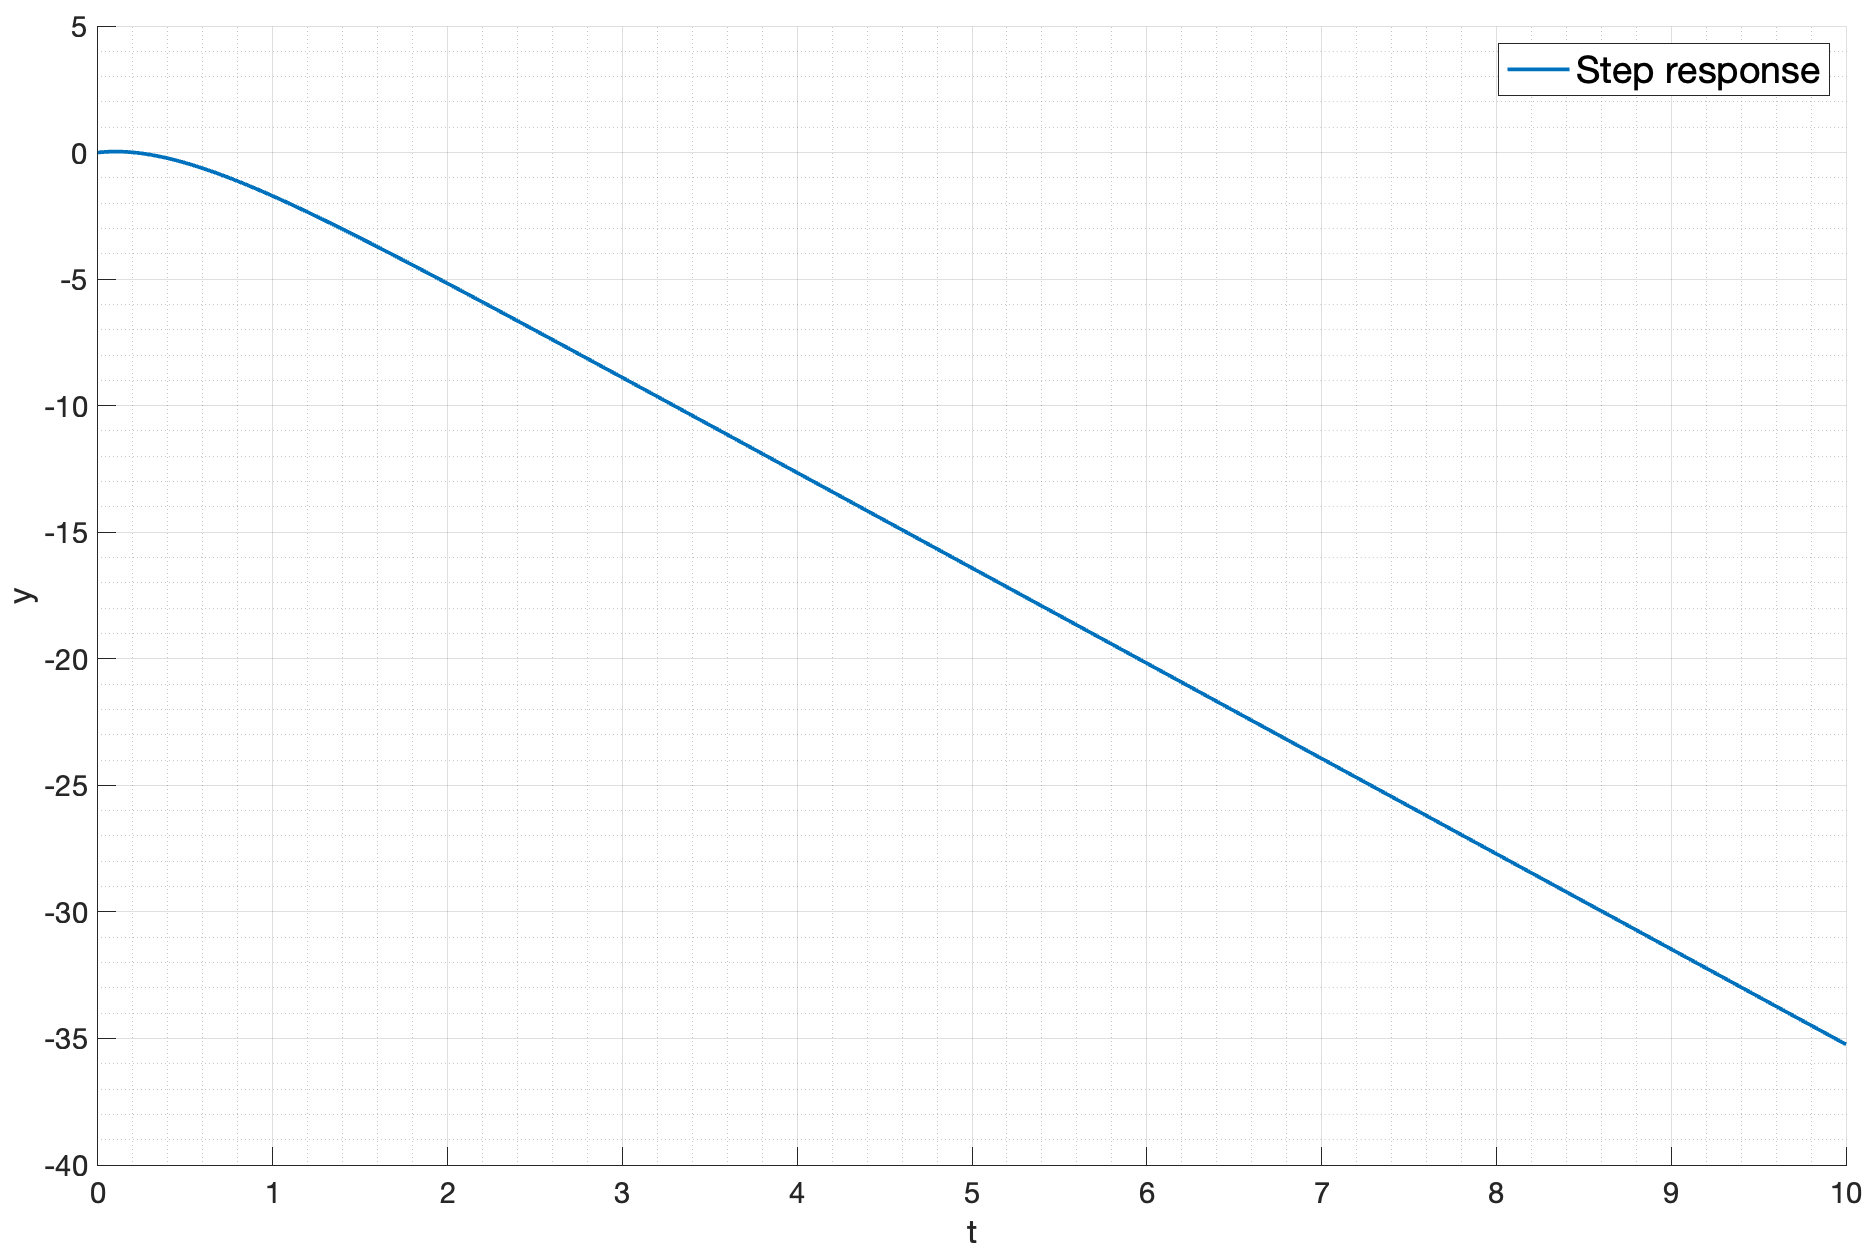
\includegraphics[width=\textwidth]{media/plots/task4_step_response_closed_5.png}
        \caption{$K = 8/9$}
    \end{subfigure}
    \caption{Переходная характеристика замкнутой системы при различных значениях коэффициента усиления $K$}
    \label{fig:task4_step}
\end{figure}

\begin{figure}[ht!]
    \begin{subfigure}{0.5\textwidth}
        \centering
        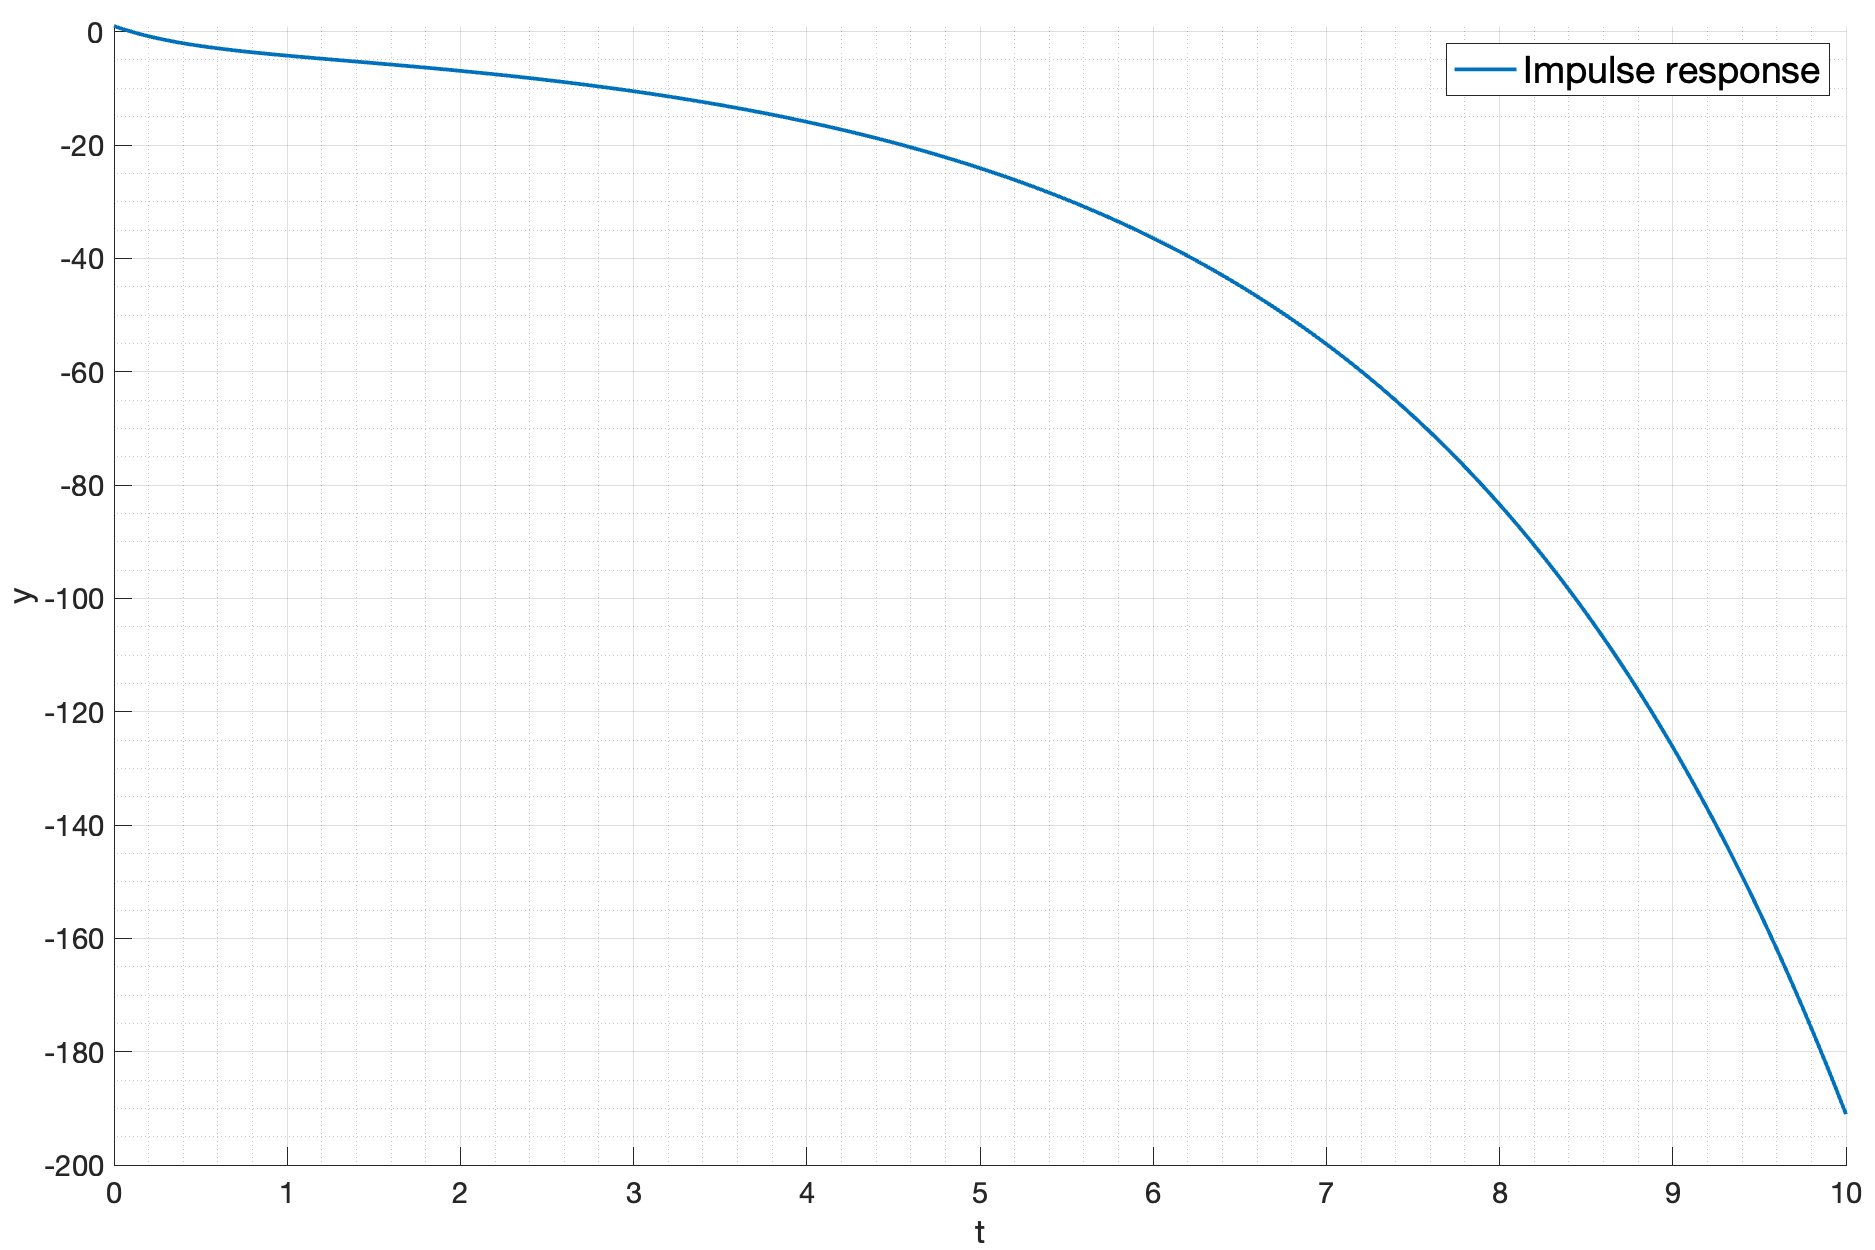
\includegraphics[width=\textwidth]{media/plots/task4_impulse_response_closed_1.png}
        \caption{$K = 1$}
    \end{subfigure}%
    \begin{subfigure}{0.5\textwidth}
        \centering
        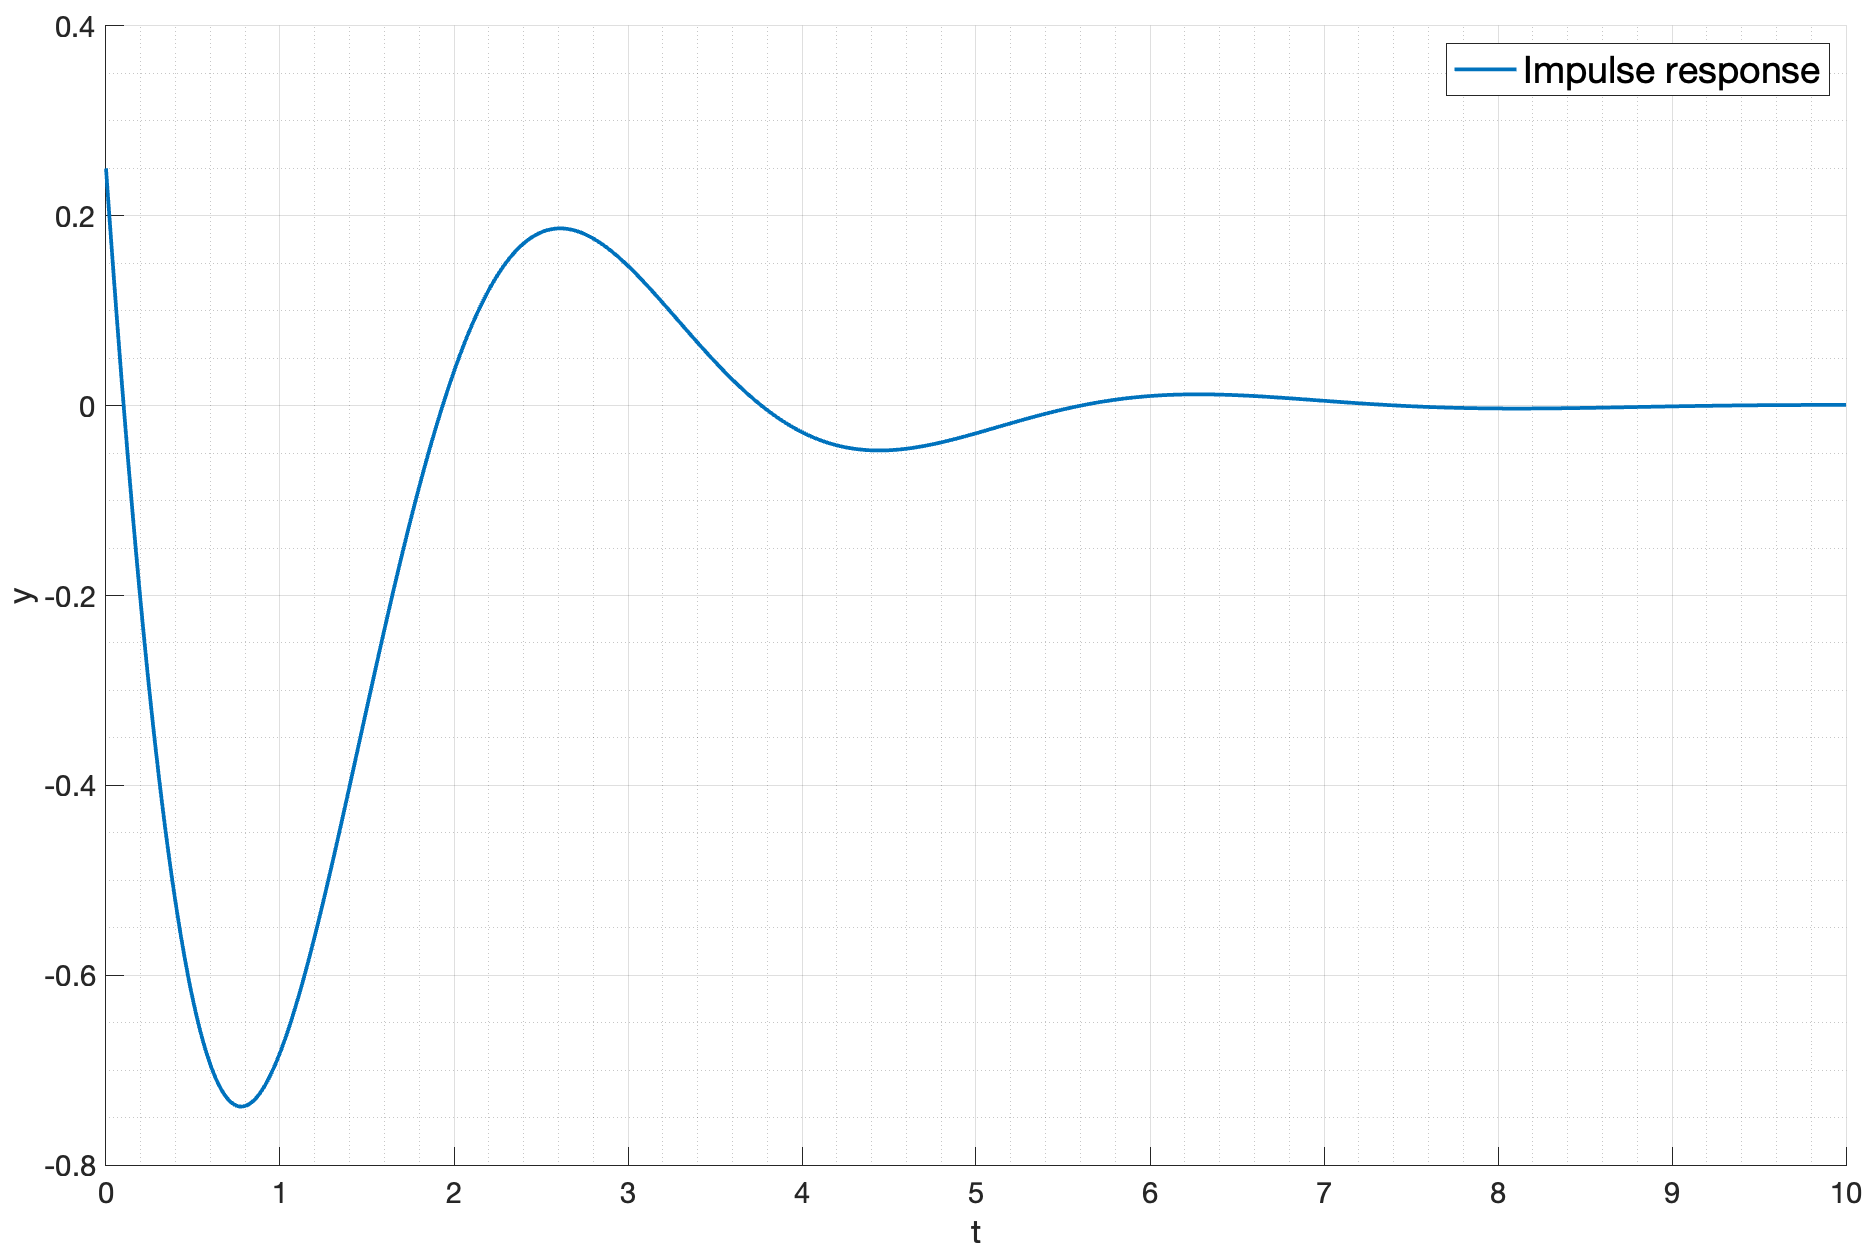
\includegraphics[width=\textwidth]{media/plots/task4_impulse_response_closed_2.png}
        \caption{$K = 0.5$}
    \end{subfigure}
    \begin{subfigure}{0.5\textwidth}
        \centering
        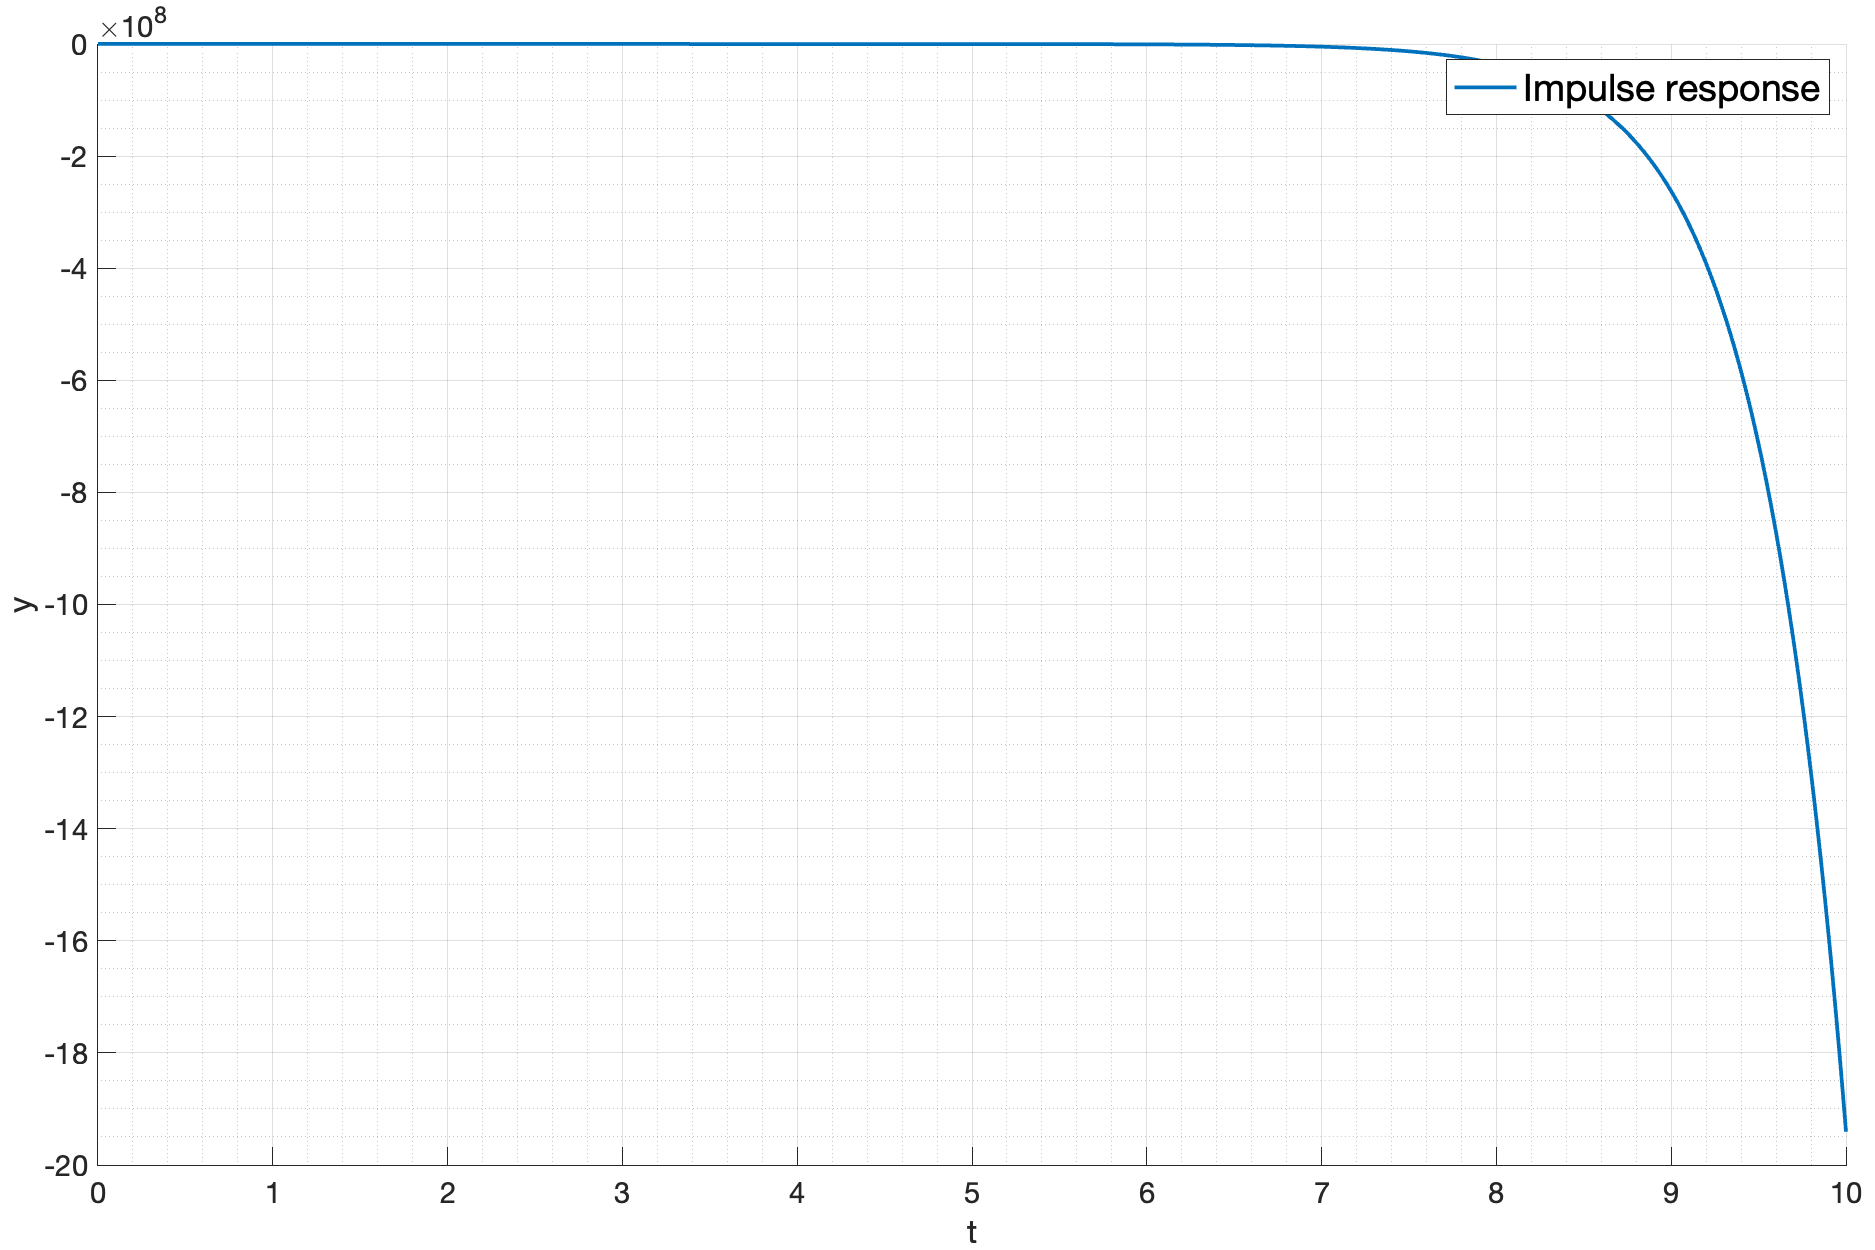
\includegraphics[width=\textwidth]{media/plots/task4_impulse_response_closed_3.png}
        \caption{$K = 2$}
    \end{subfigure}%
    \begin{subfigure}{0.5\textwidth}
        \centering
        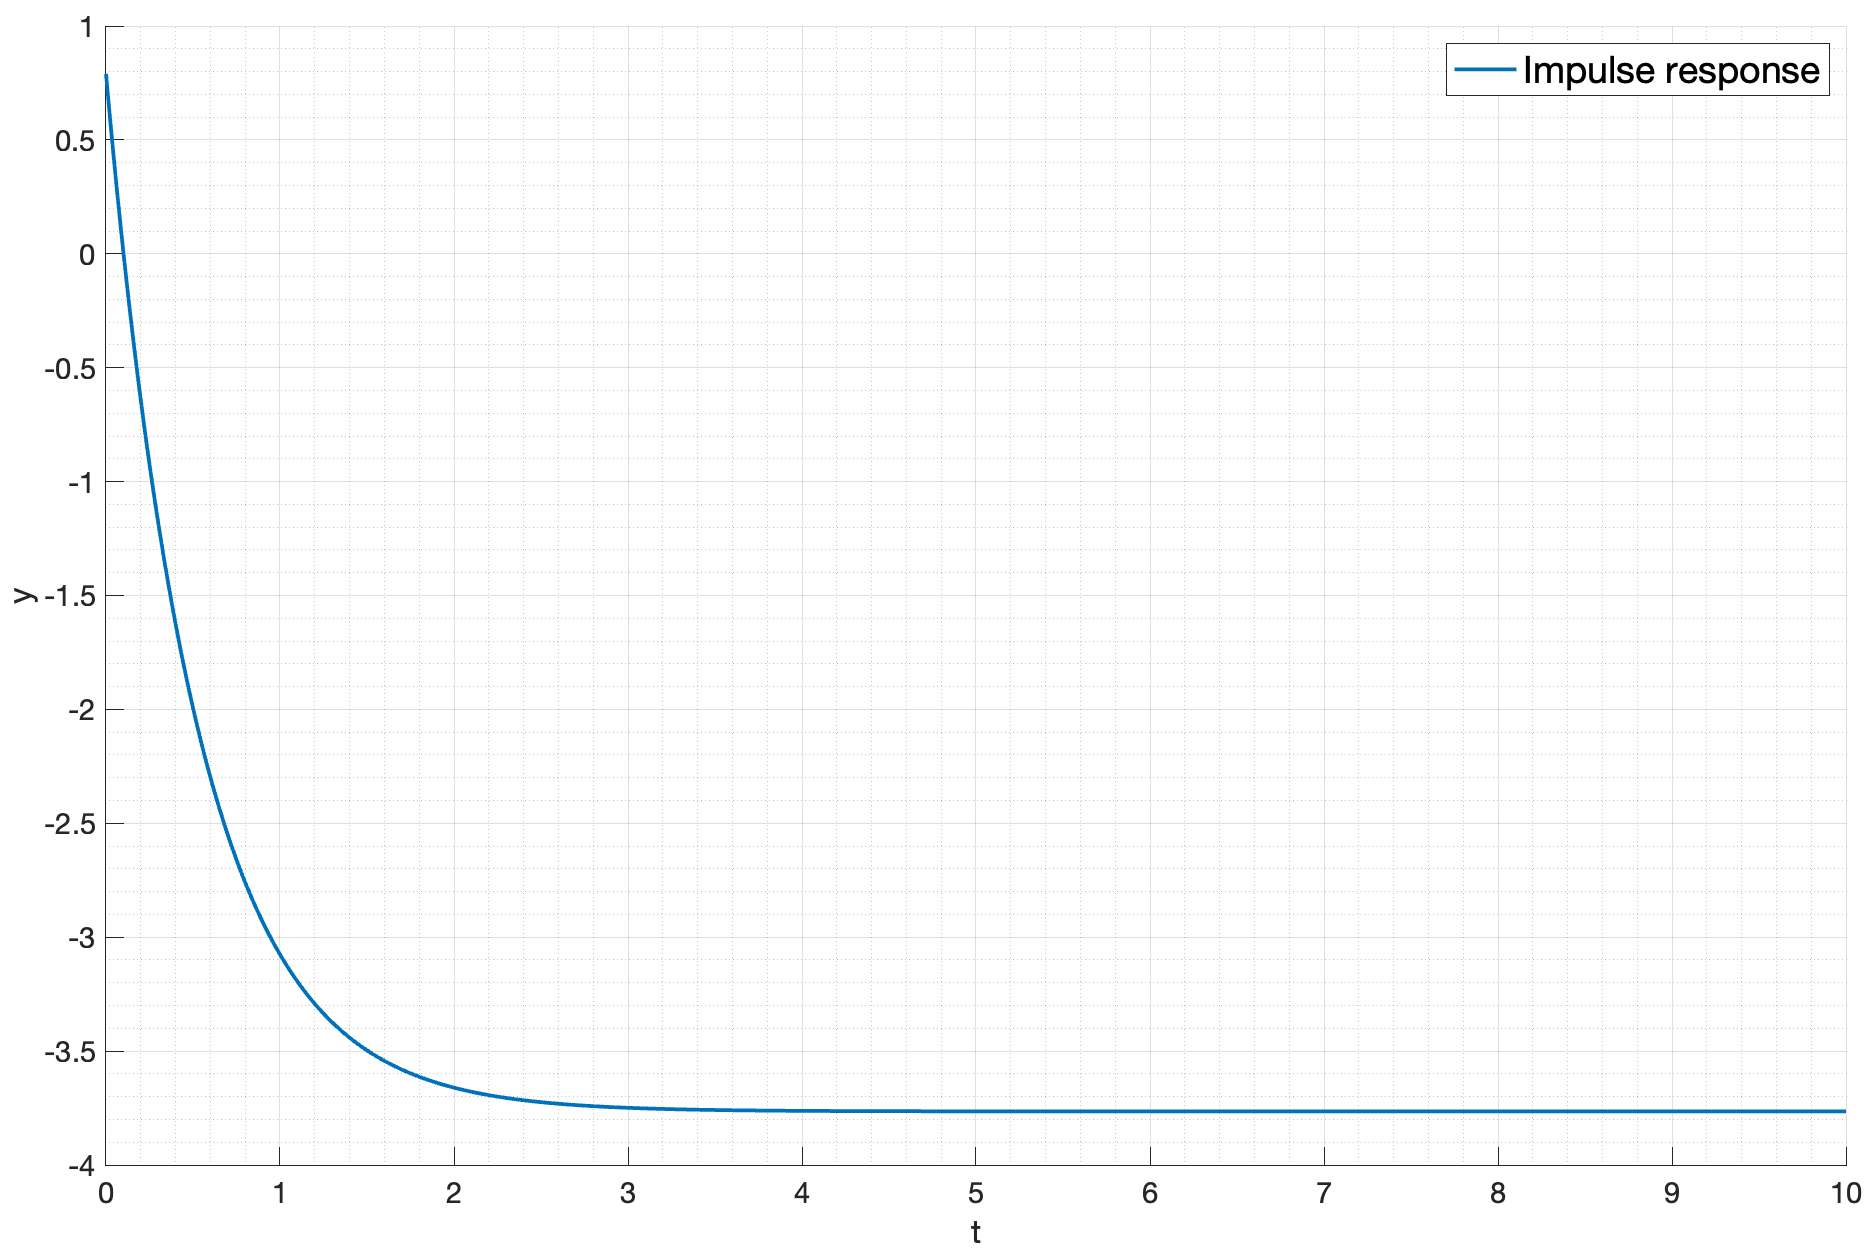
\includegraphics[width=\textwidth]{media/plots/task4_impulse_response_closed_5.png}
        \caption{$K = 8/9$}
    \end{subfigure}
    \caption{Импульсная характеристика замкнутой системы при различных значениях коэффициента усиления $K$}
    \label{fig:task4_impulse}
\end{figure}
При значениях $K$ меньше критического значения $8/9$ выход системы сходится к постоянной величине,
при значениях $K$ больше критического значения $8/9$ выход системы расходится, 
а при значениях $K$ равных критическому значению $8/9$ выход убывает пропорционально времени.

\subsection{Система 2}
Рассмотрим объект, заданный передаточной функцией:
\begin{eqnarray}
    W_2(s) = \frac{K(-80s^3+80s^2+3s-0.04)}{100s^3-20s^2-2s+0.3}
\end{eqnarray}

Построим годограф Найквиста для этой системы при различных значениях коэффициента усиления $K$ (см. рис. \ref{fig:task5_nyquist}).
\begin{figure}[ht!]
    \begin{subfigure}{0.5\textwidth}
        \centering
        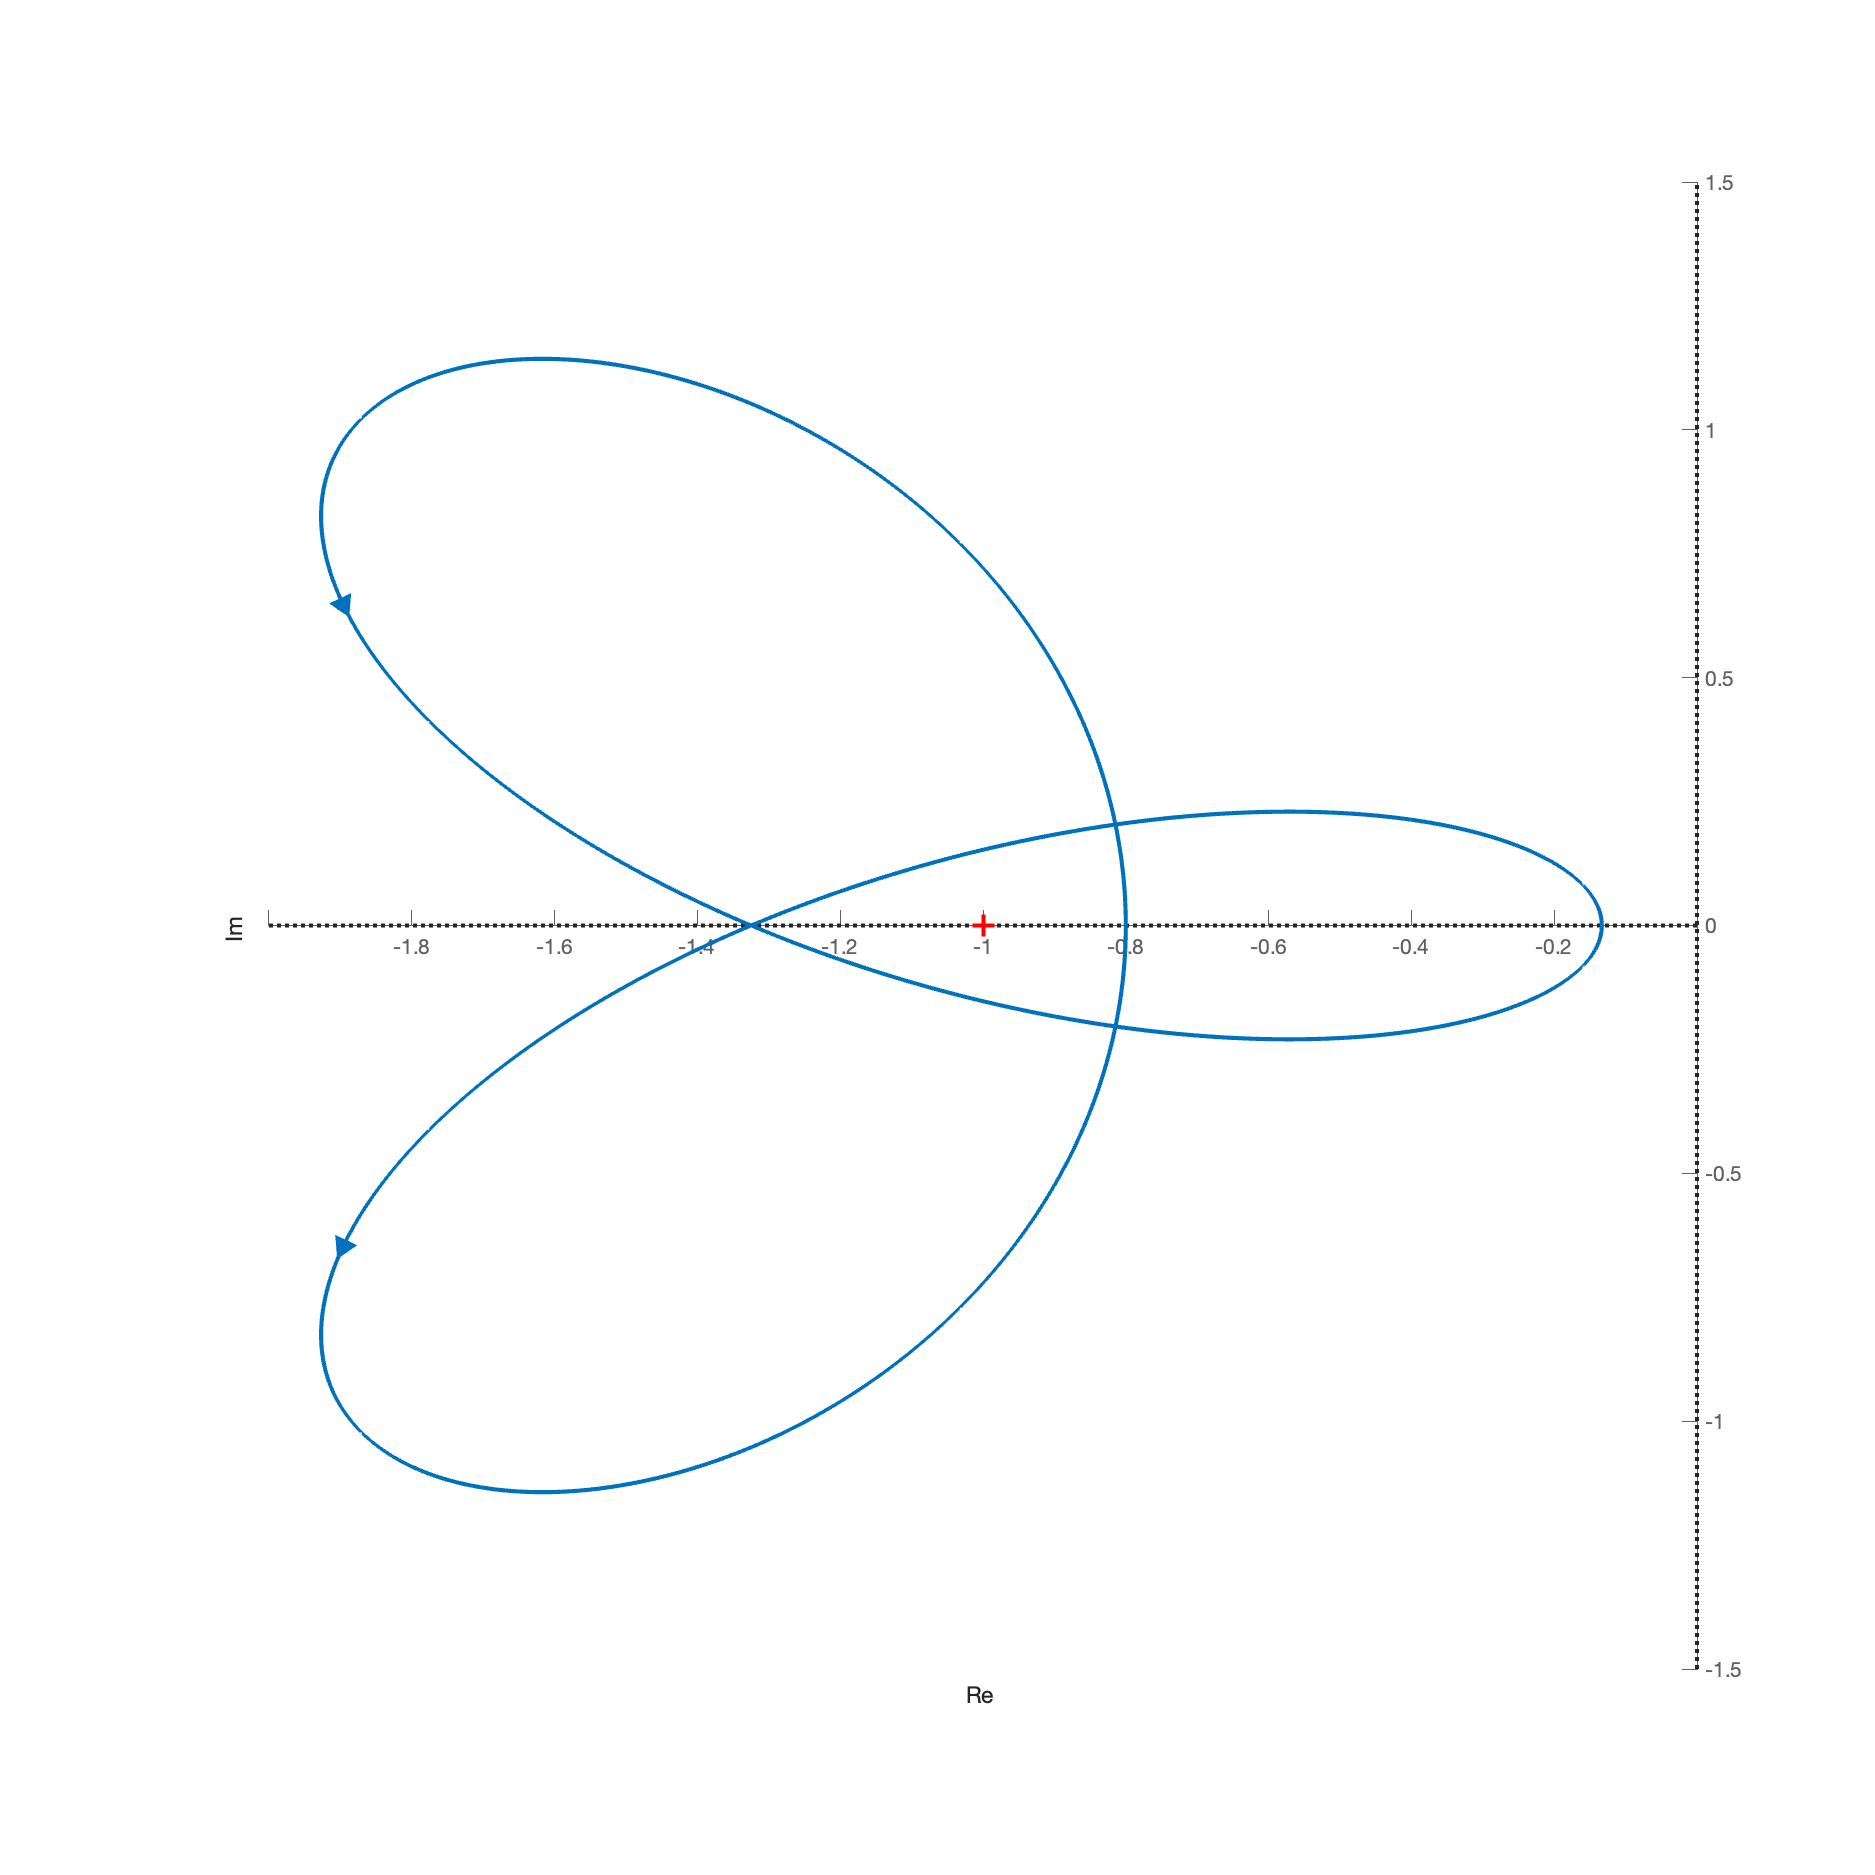
\includegraphics[width=\textwidth]{media/plots/task5_nyquist_1.png}
        \caption{$K = 1$}
    \end{subfigure}
    \begin{subfigure}{0.5\textwidth}
        \centering
        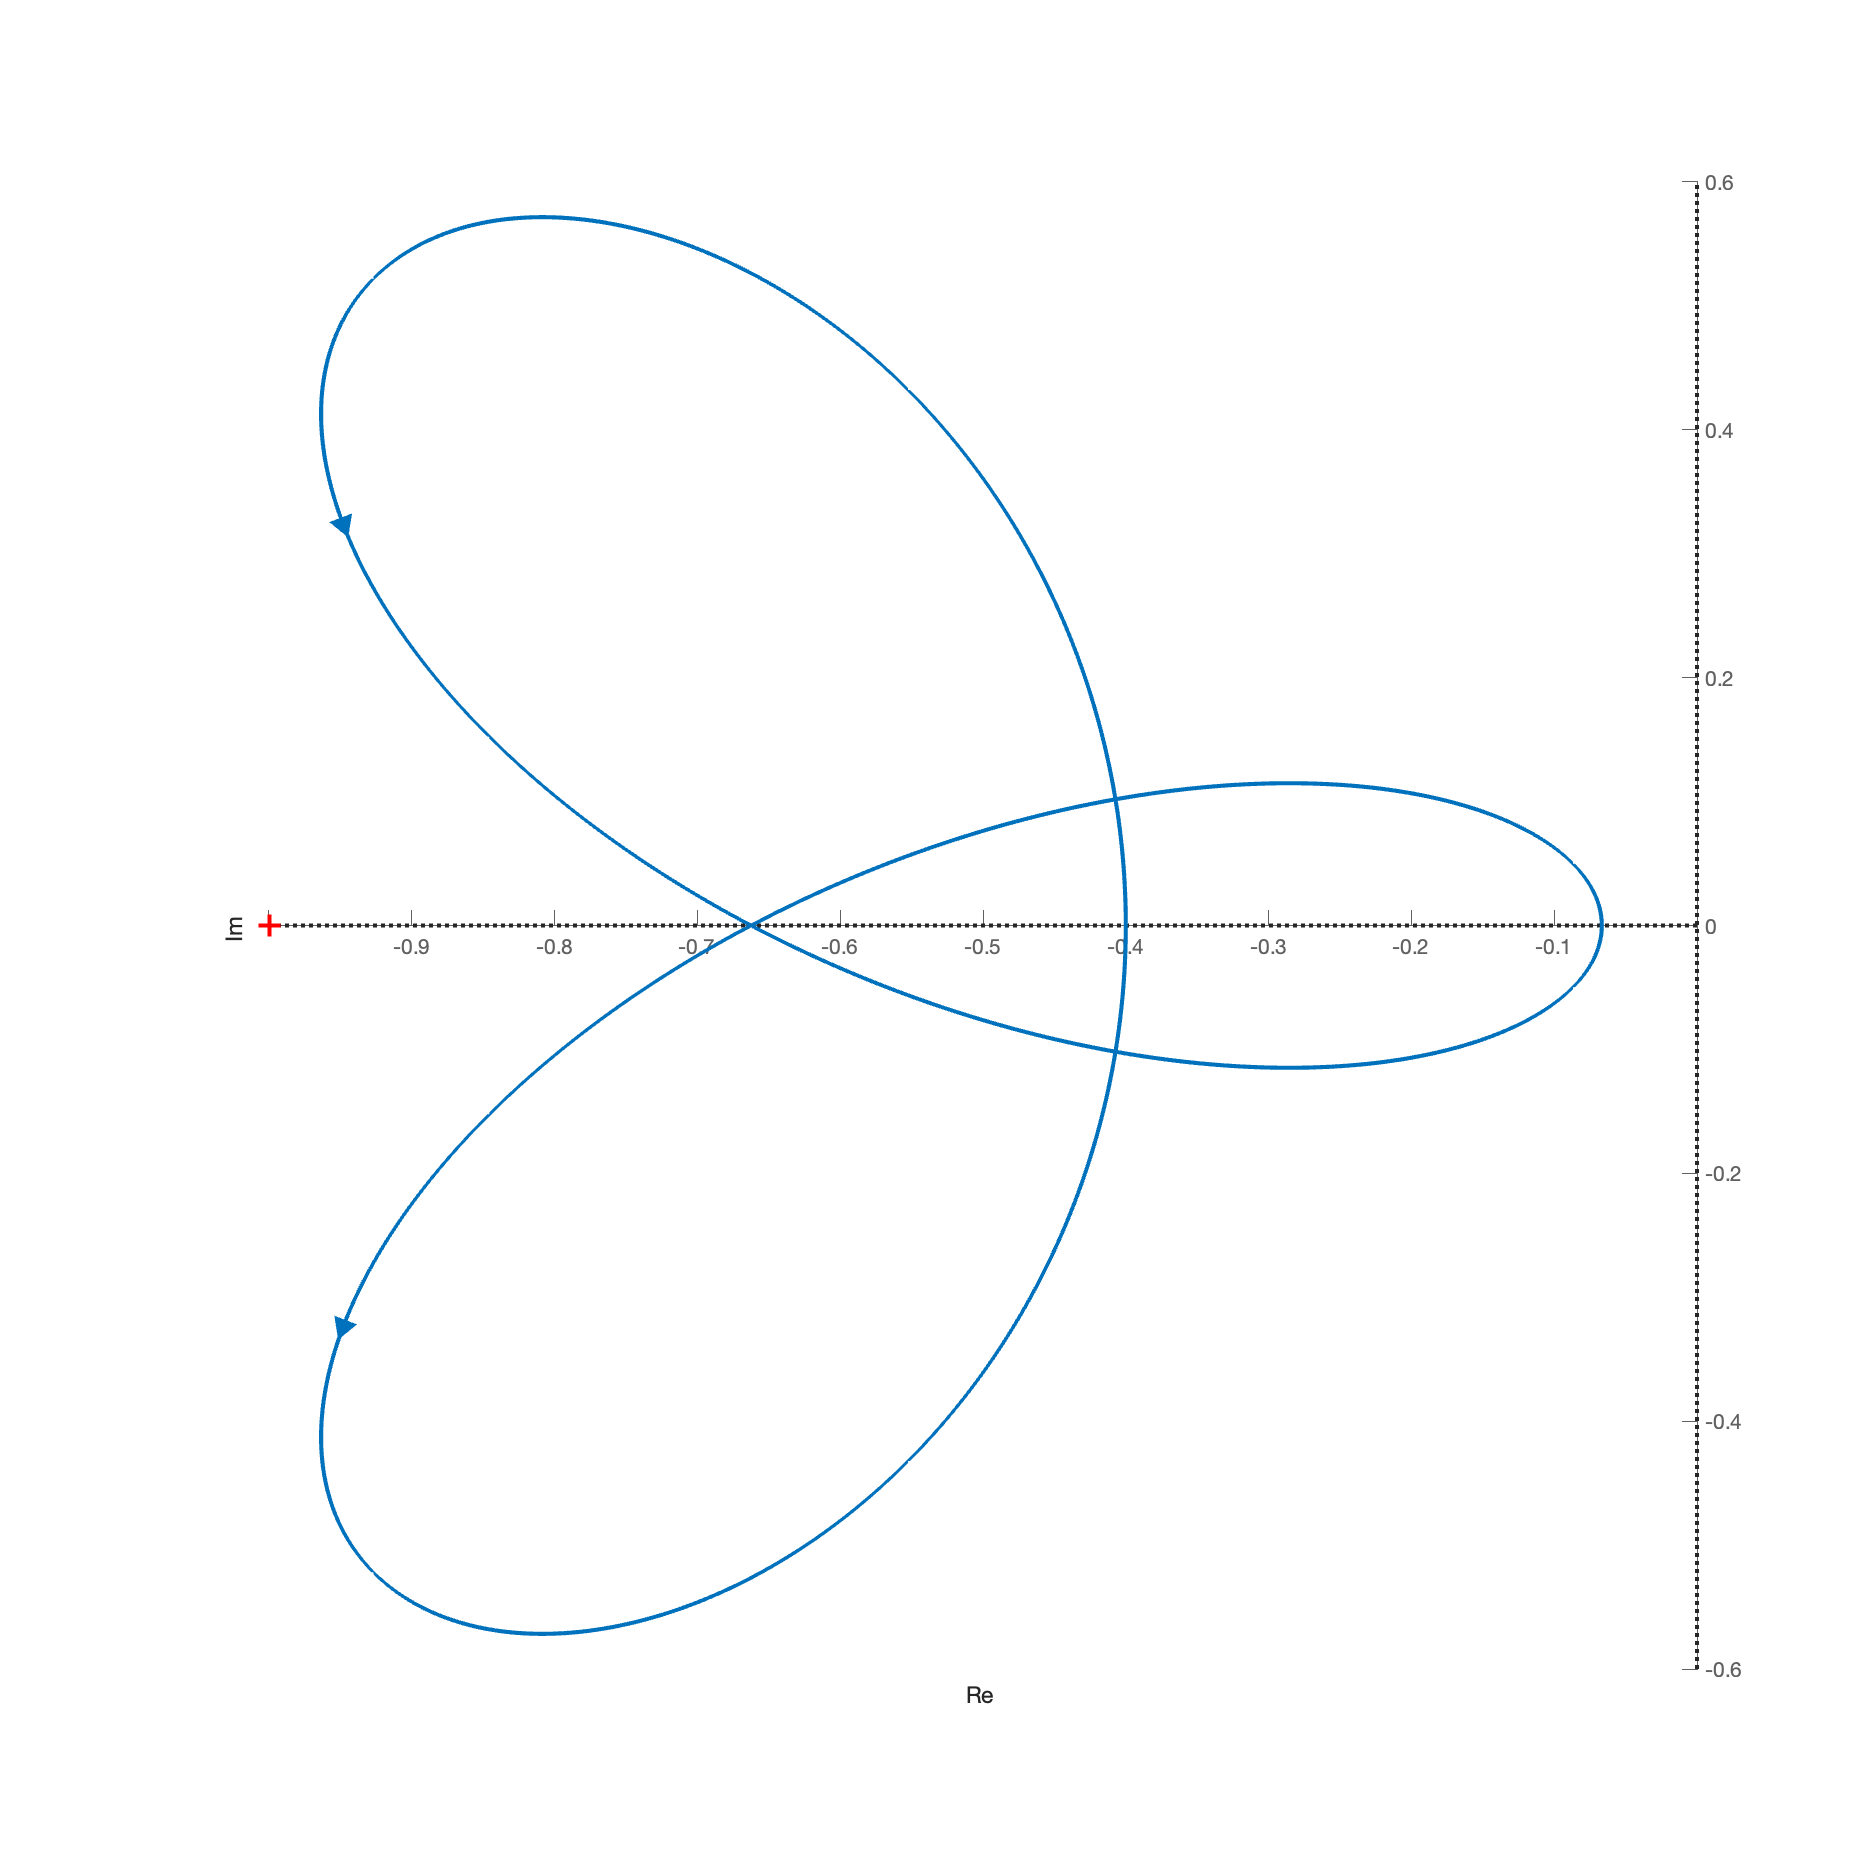
\includegraphics[width=\textwidth]{media/plots/task5_nyquist_2.png}
        \caption{$K = 0.5$}
    \end{subfigure}
    \begin{subfigure}{0.5\textwidth}
        \centering
        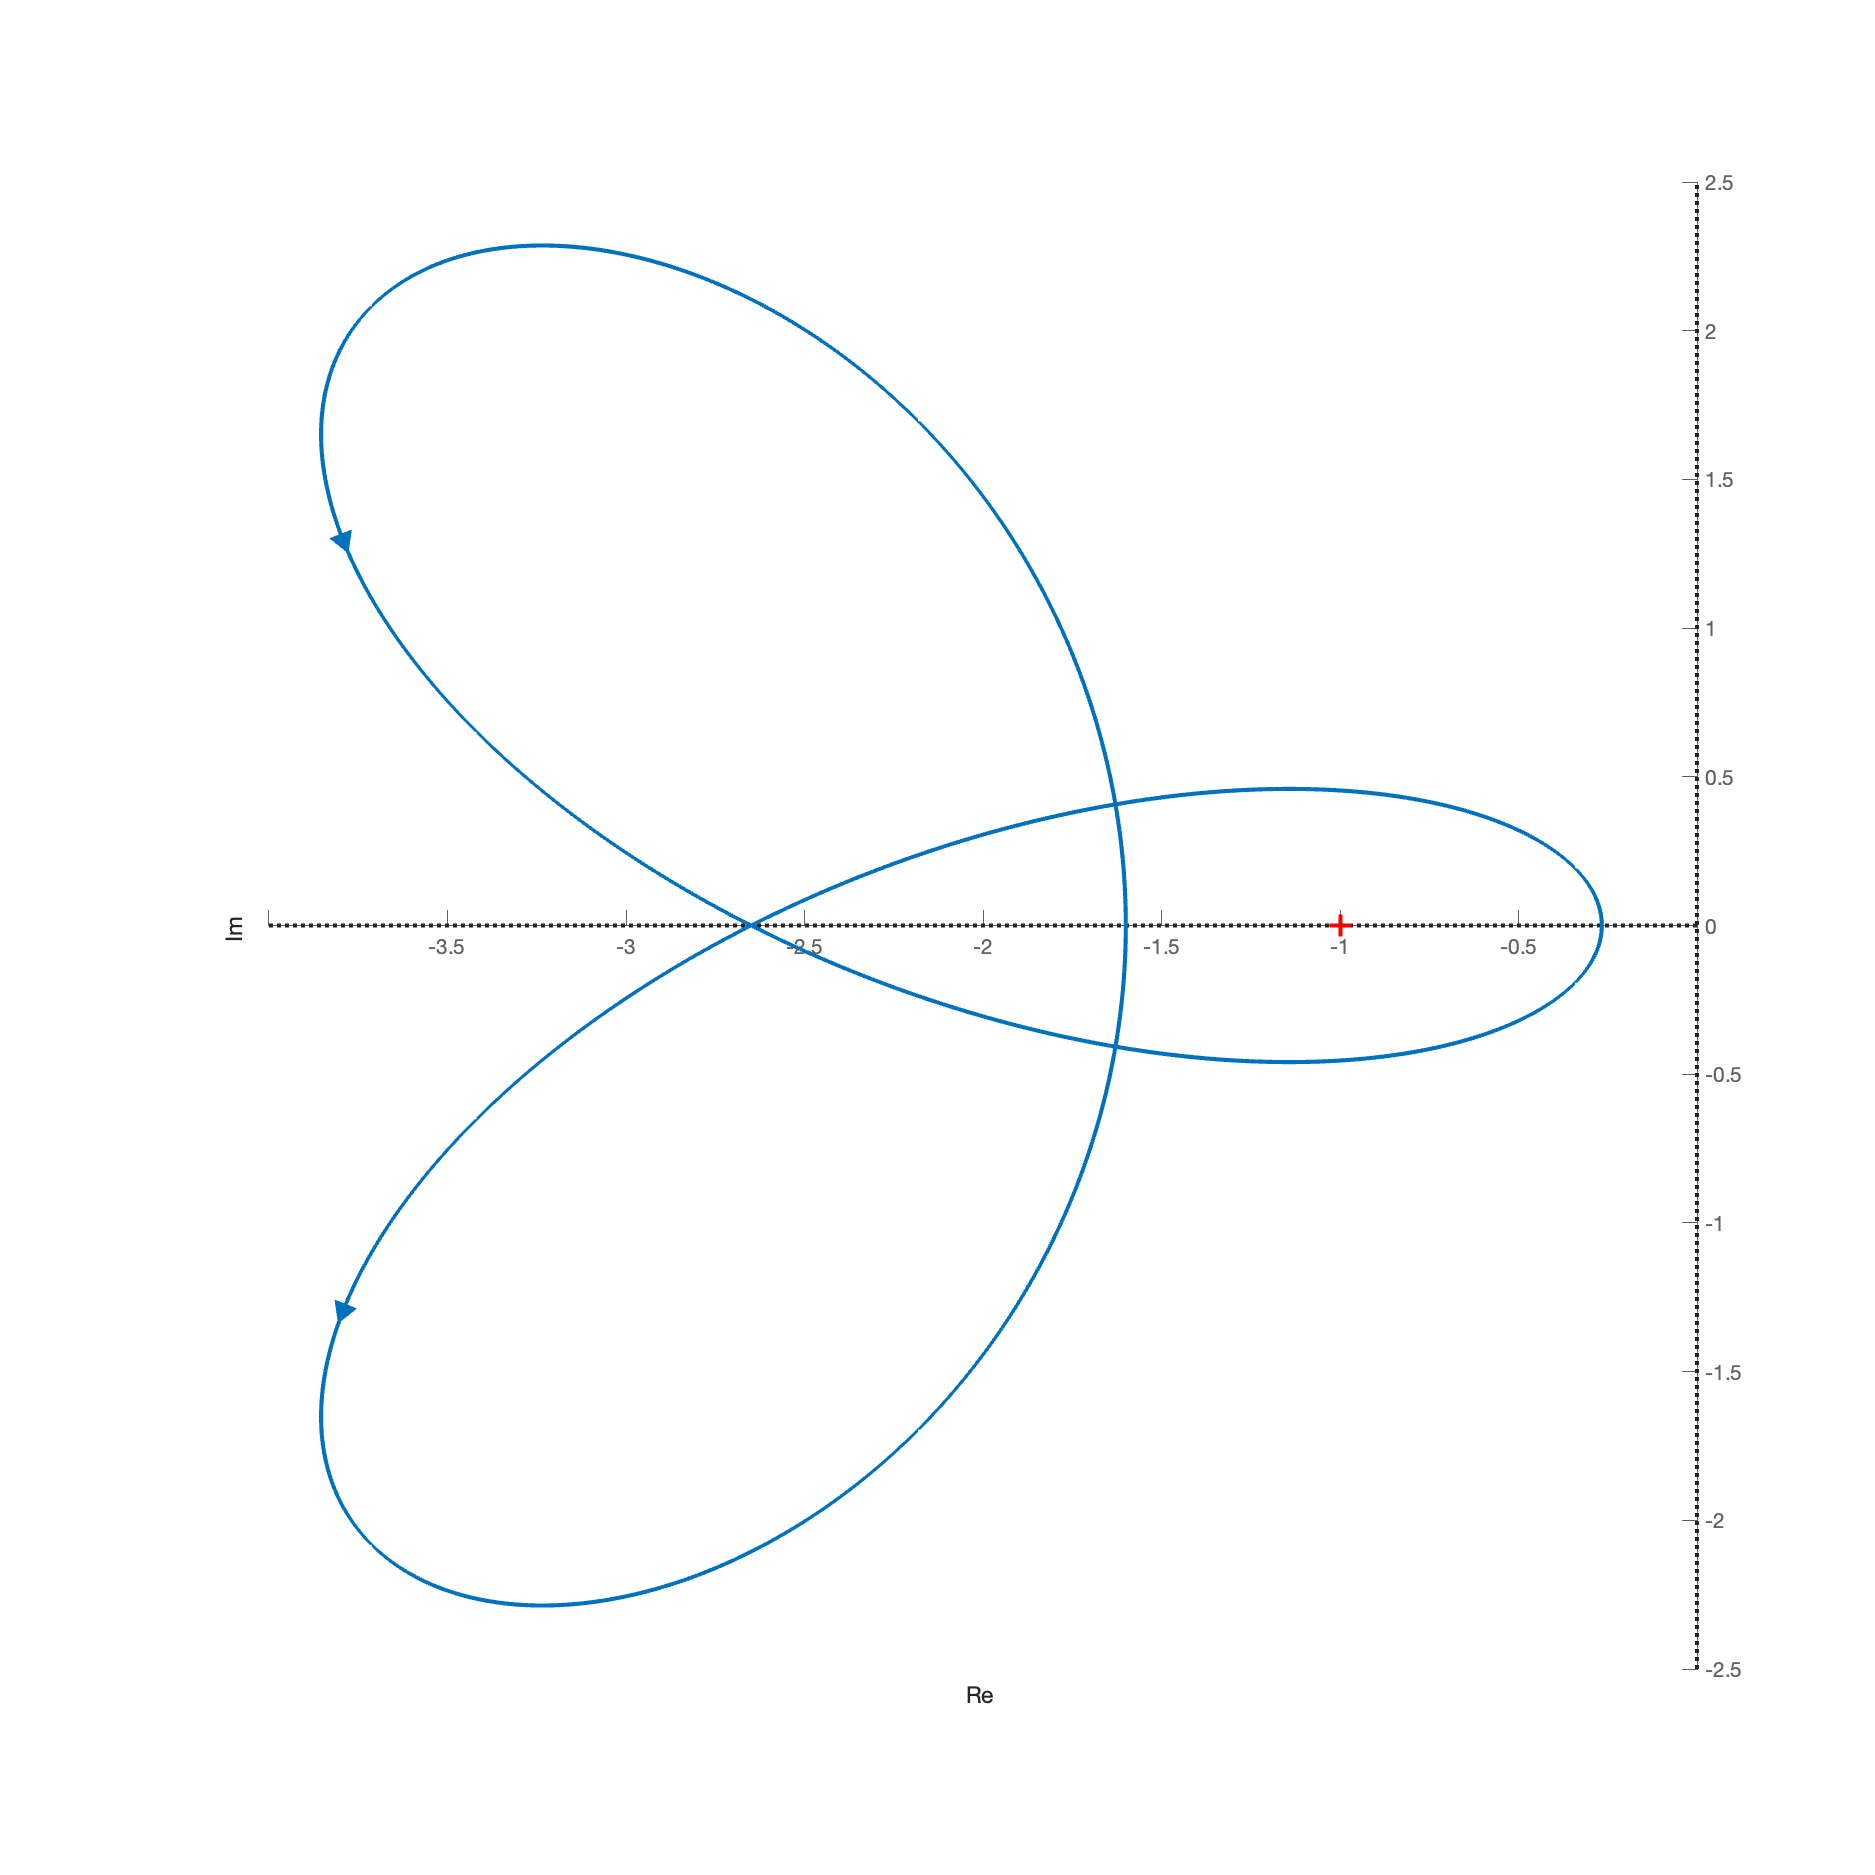
\includegraphics[width=\textwidth]{media/plots/task5_nyquist_3.png}
        \caption{$K = 2$}
    \end{subfigure}
    \begin{subfigure}{0.5\textwidth}
        \centering
        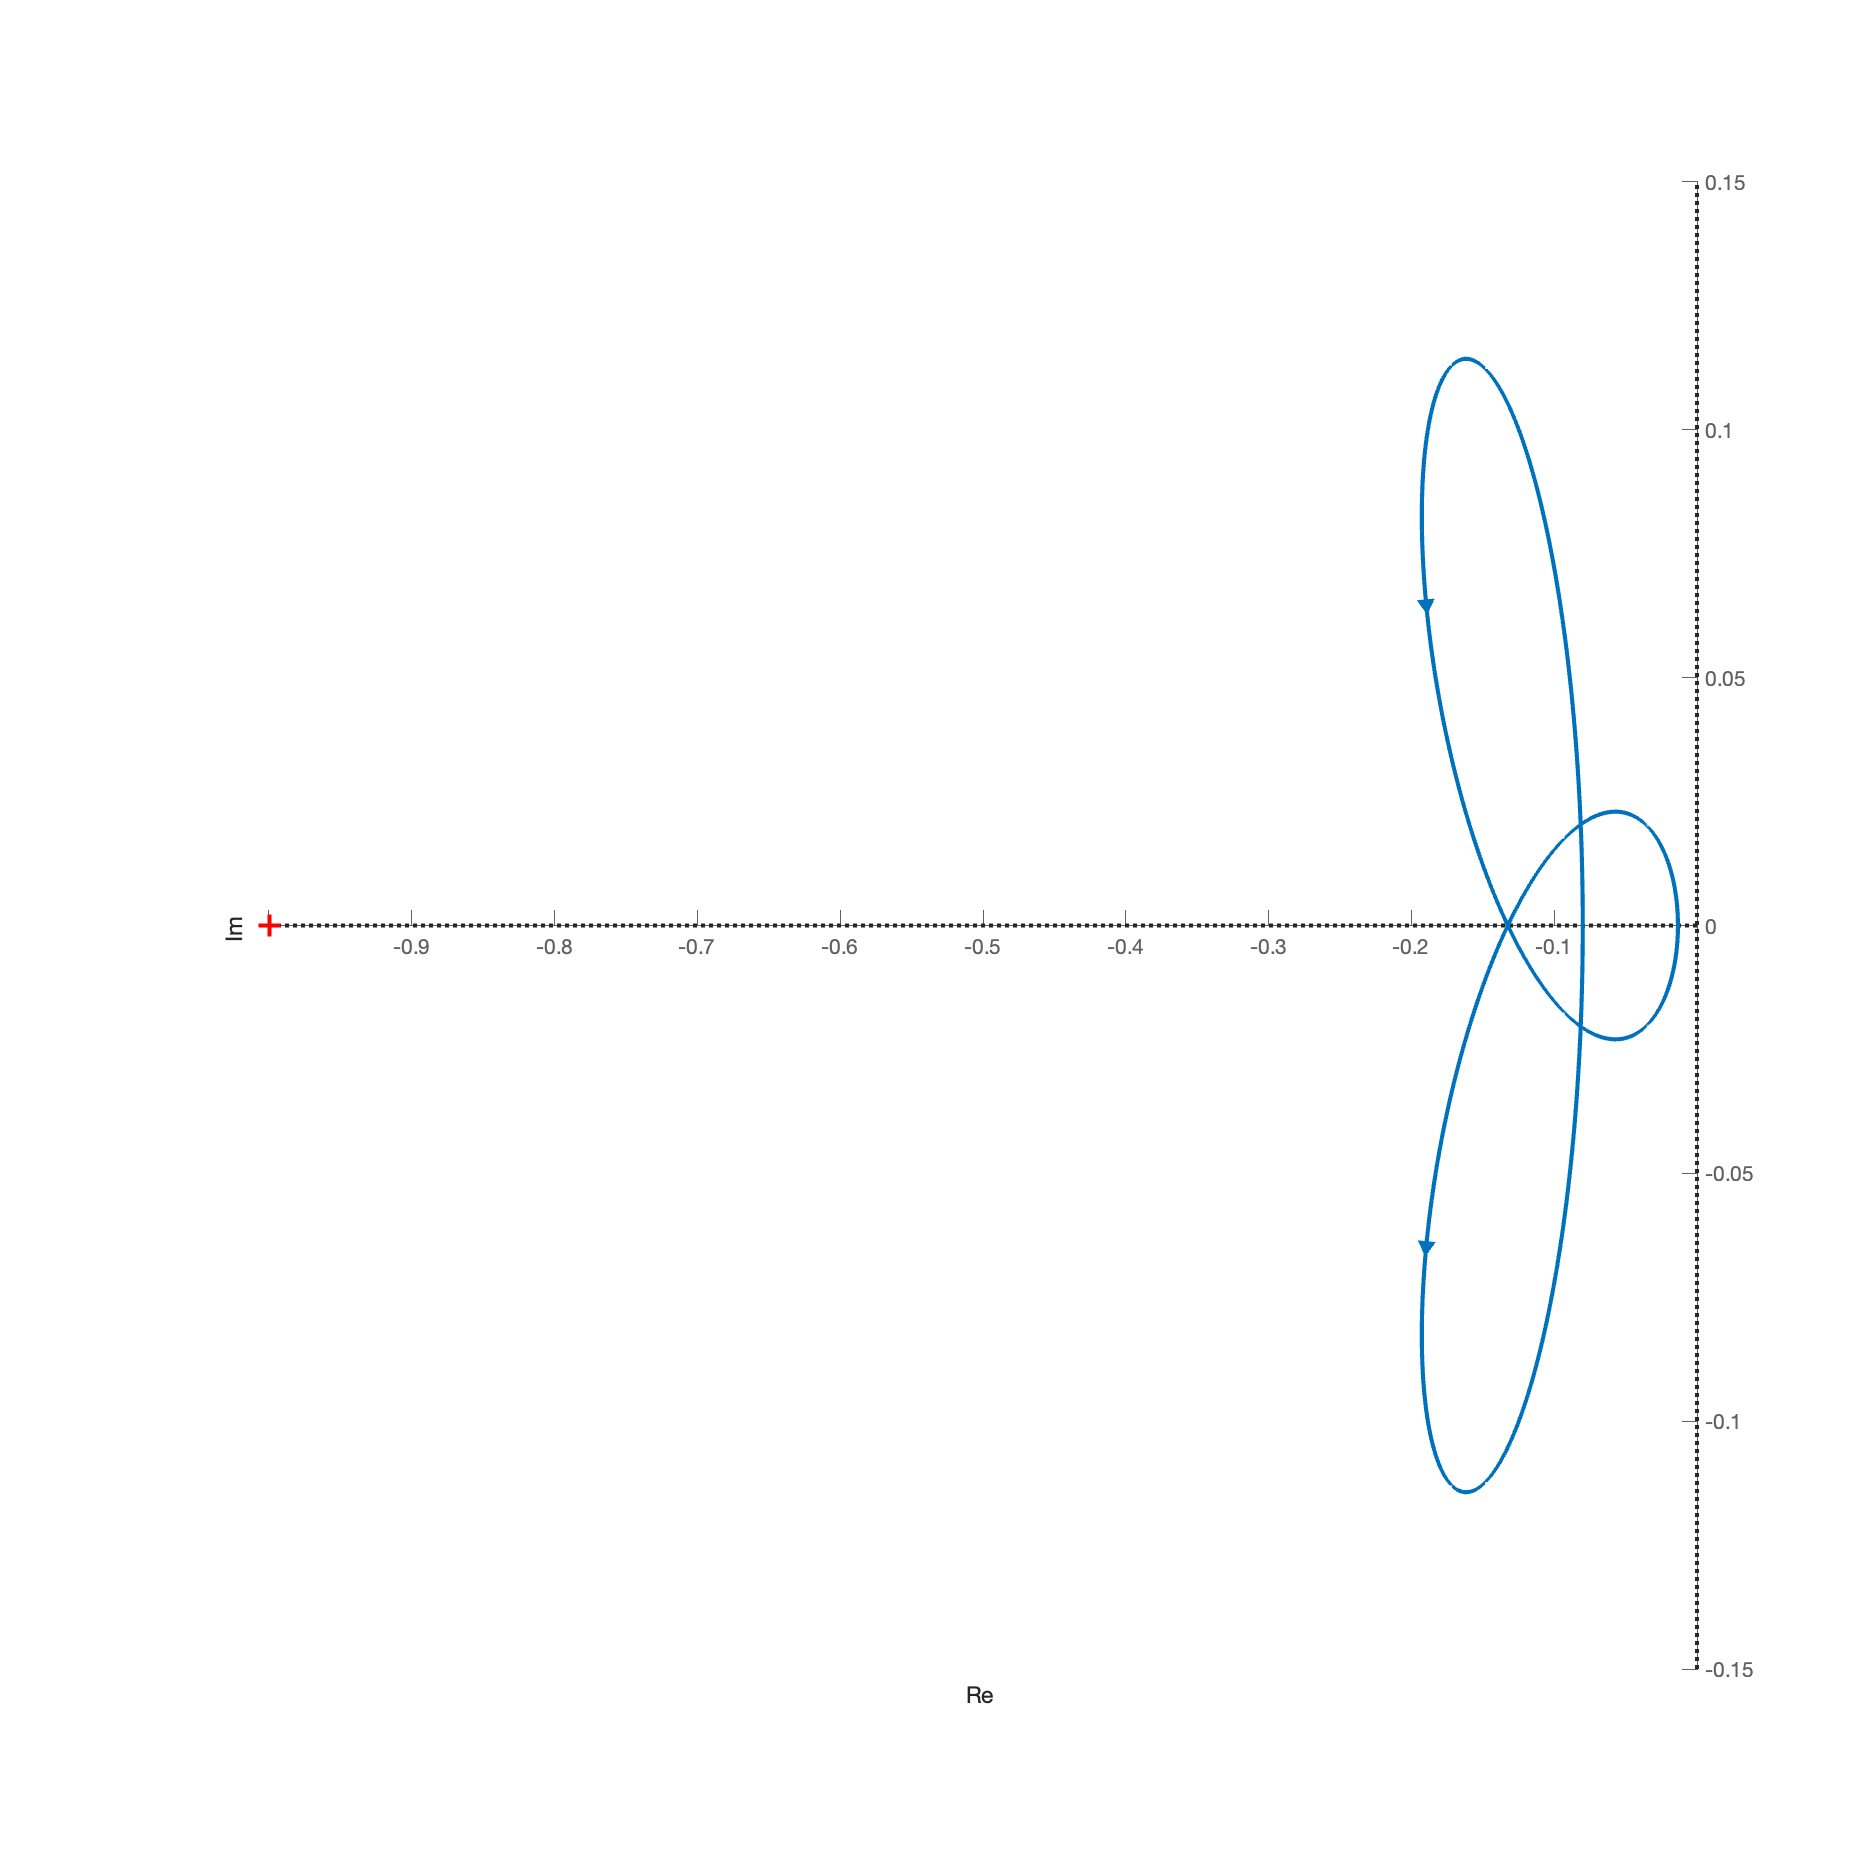
\includegraphics[width=\textwidth]{media/plots/task5_nyquist_4.png}
        \caption{$K = 0.1$}
    \end{subfigure}
    \caption{Годограф Найквиста для различных значений коэффициента усиления $K$}
    \label{fig:task5_nyquist}
\end{figure}

Как и в прошлом случае, видно, что при увеличении значения коэффициента усиления $K$ годограф \textit{растягивается} по горизонтали и вертикали,
при $K$ больших 0.75 задевая точку $(-1, 0)$, делая два оборота против часовой стрелки вокруг нее, таким образом, компенсирую неустойчивость разомкнутой системы.
При значениях $K$ более 1.25, уде другая часть годографа задевает точку $(-1, 0)$, в итоге оставляя только один оборот против часовой стрелки вокруг нее.
Таким образом, при $K > 1.25$ система становится неустойчивой с одни полюсом с положительной вещественной частью.
При значениях $K$ более 7.5 годограф вновь перестает задевать точку $(-1, 0)$, в системе снова появляются два неустойчивых полюса. 

Разомкнутая система имеет полюса:
\begin{equation}
    s_1 \approx -0.13 \quad s_2 \approx 0.1 \quad s_3 \approx 0.23 
\end{equation}
Разомкнутая система не является устойчивой, так как имеет два полюса с положительной вещественной частью. 

Передаточная функция замкнутой системы:
\begin{equation}
    W_{2c}(s) = \frac{K(-80s^3+80s^2+3s-0.04)}{(100 - 80K)s^3 + (-20 + 80K)s^2 + (-2 + 3K)s + 0.3 - 0.04K} 
\end{equation}
% \begin{equation}
%     W_{2c}(s) = \frac{\frac{-80s^3+80s^2+3s-0.04}{100s^3-20s^2-2s+0.3}}{1 + \frac{-80s^3+80s^2+3s-0.04}{100s^3-20s^2-2s+0.3}} = \frac{-80s^3+80s^2+3s-0.04}{100s^3-20s^2-2s+0.3 - 80s^3+80s^2+3s-0.04}
% \end{equation}
Найдем значения коэффициента усиления $K$, при которых замкнутая система будет устойчивой согласно 
следствию из критерия Гурвица для систем третьего порядка:
\begin{multline}
    \begin{cases}
        100 - 80K > 0 \\
        -20 + 80K > 0 \\
        -2 + 3K > 0 \\
        0.3 - 0.04K > 0 \\ 
       (-20 + 80K)(-2 + 3K) - (100 - 80K)(0.3 - 0.04K) > 0
    \end{cases} 
    \Rightarrow \begin{cases}
        K < \frac{5}{4} \\
        K > \frac{1}{4} \\
        K > \frac{2}{3} \\
        K < \frac{15}{2} \\
        K > \frac{1}{148}(60 - 5\sqrt{107})
    \end{cases} \\  \Rightarrow K \in \left(\frac{1}{148}(60 - 5\sqrt{107}), \frac{5}{4}\right) \approx (0.75, 1.25)
\end{multline}
\pagebreak
Таким образом, замкнутая система будет устойчивой при $K \in (0.75, 1.25)$.
Годограф Найквиста при критических значениях коэффициента усиления $K = 0.75$, $K = 1.25$ и $K = 7.5$ представлен на рис. \ref{fig:task5_nyquist_critical}.
\begin{figure}[ht!]
    \centering
    \begin{subfigure}{0.5\textwidth}
        \centering
        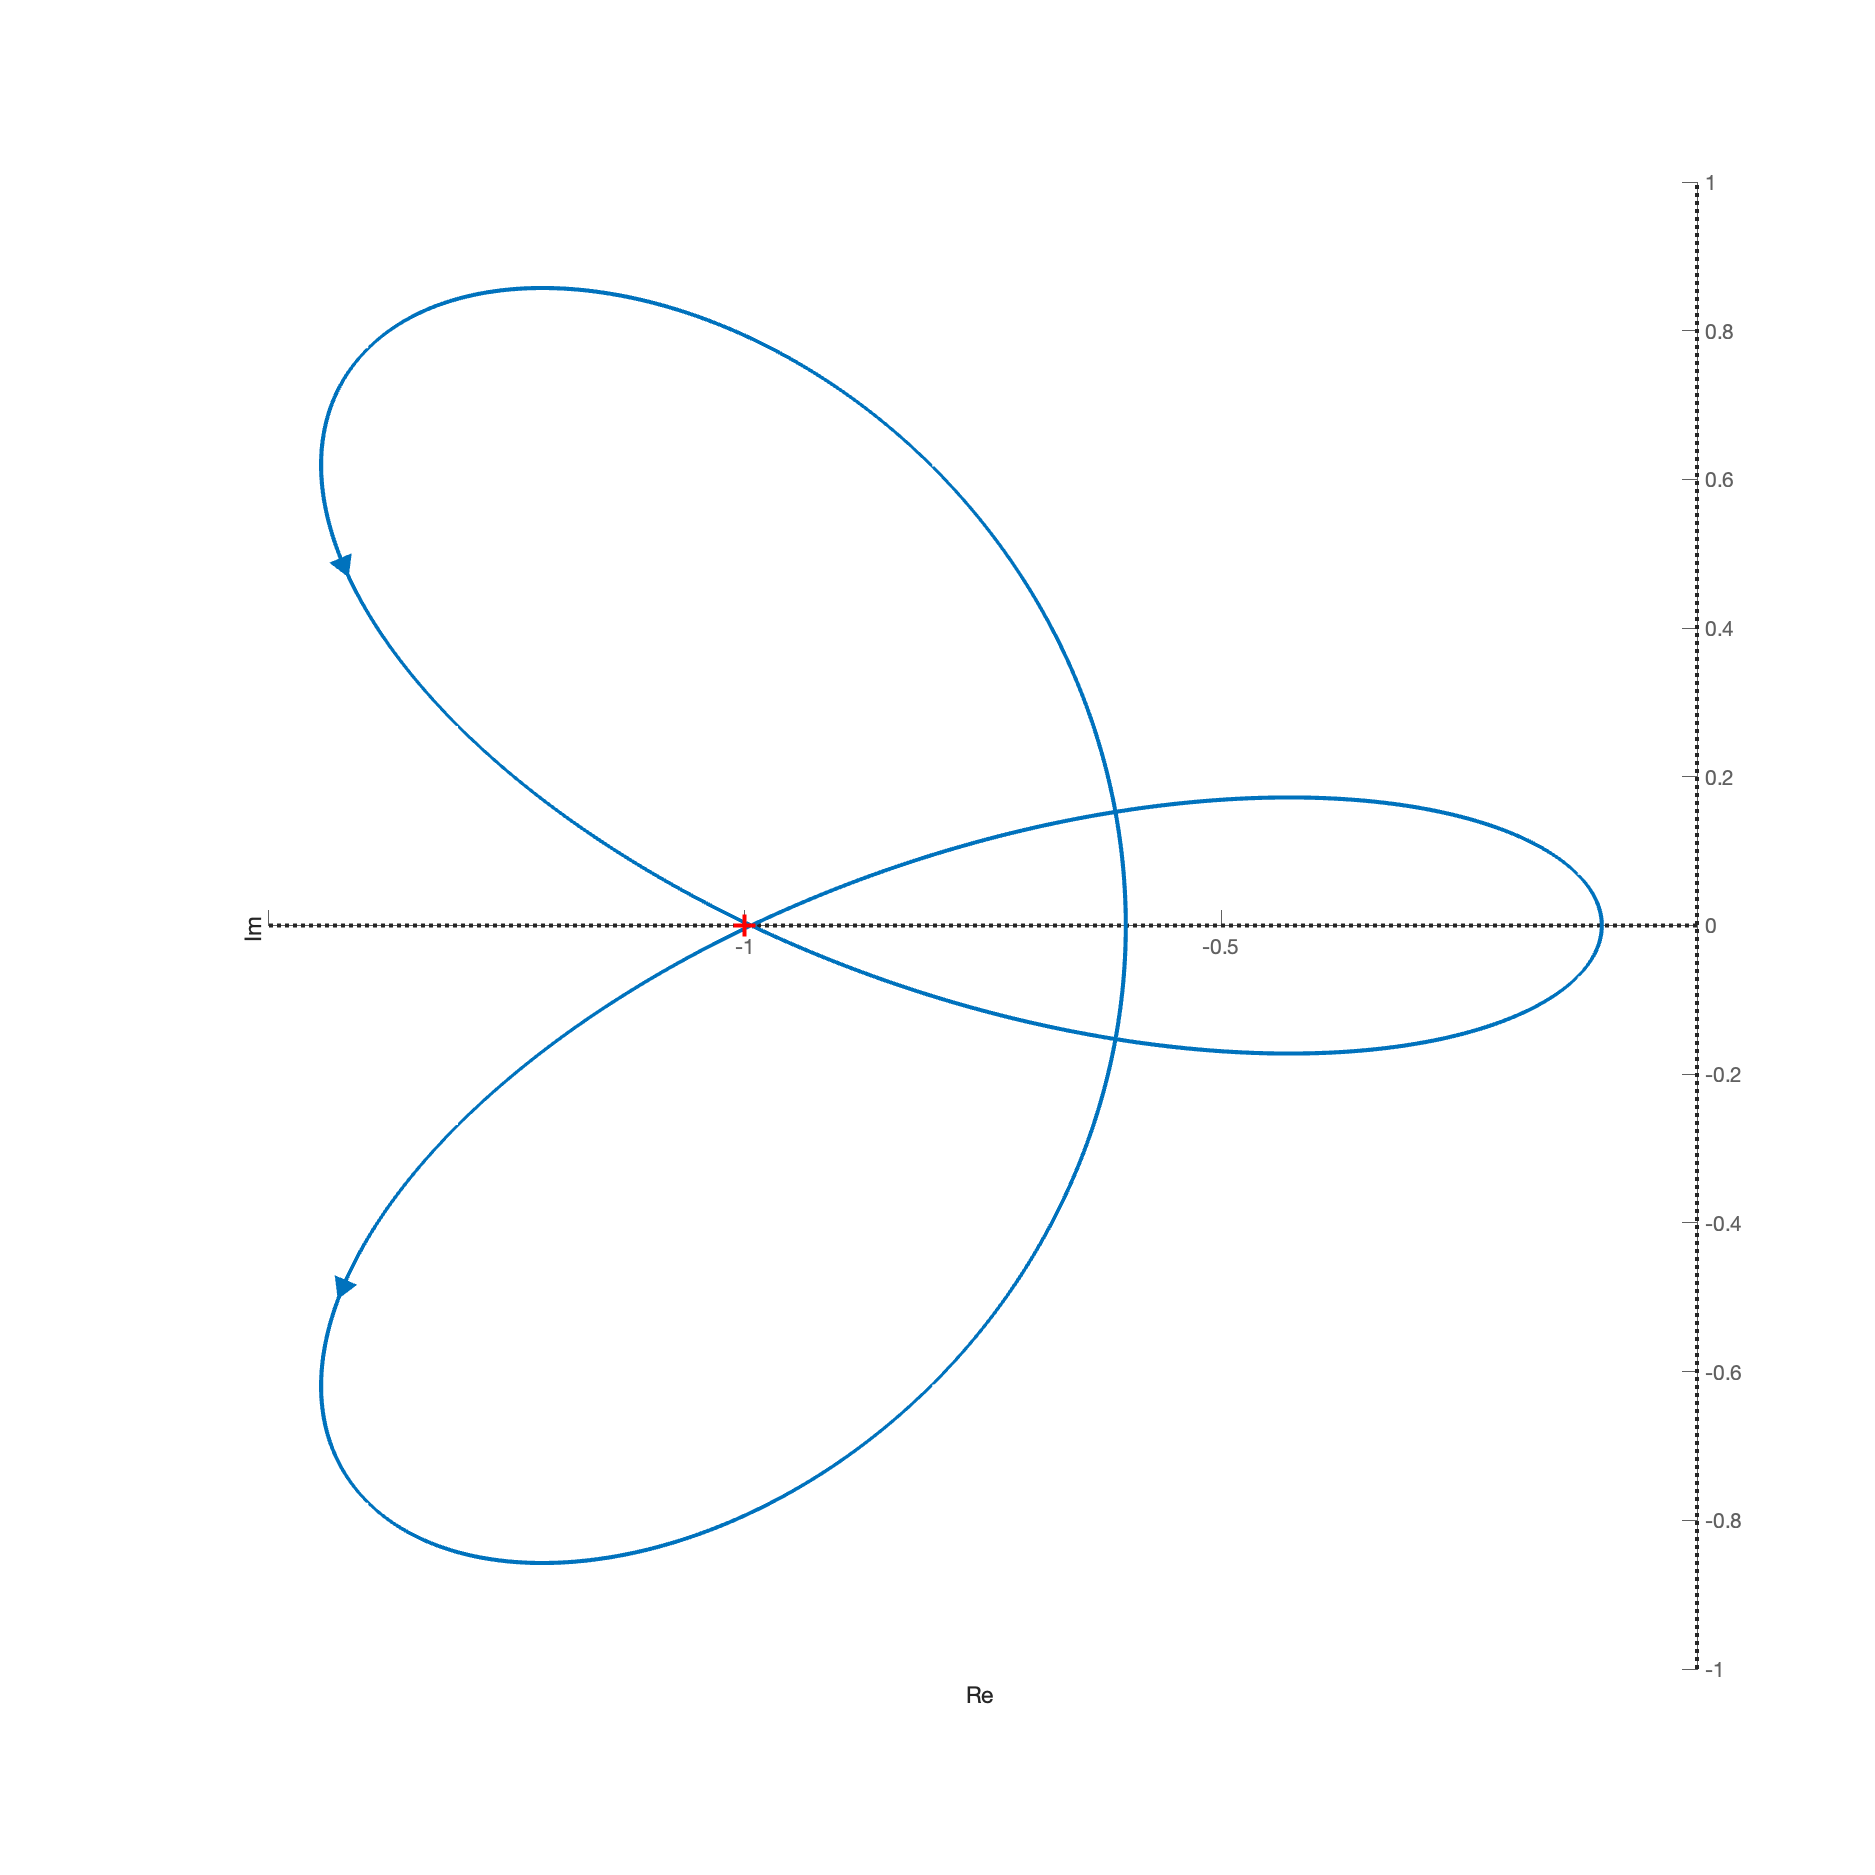
\includegraphics[width=\textwidth]{media/plots/task5_nyquist_5.png}
        \caption{$K = 0.75$}
    \end{subfigure}%
    \begin{subfigure}{0.5\textwidth}
        \centering
        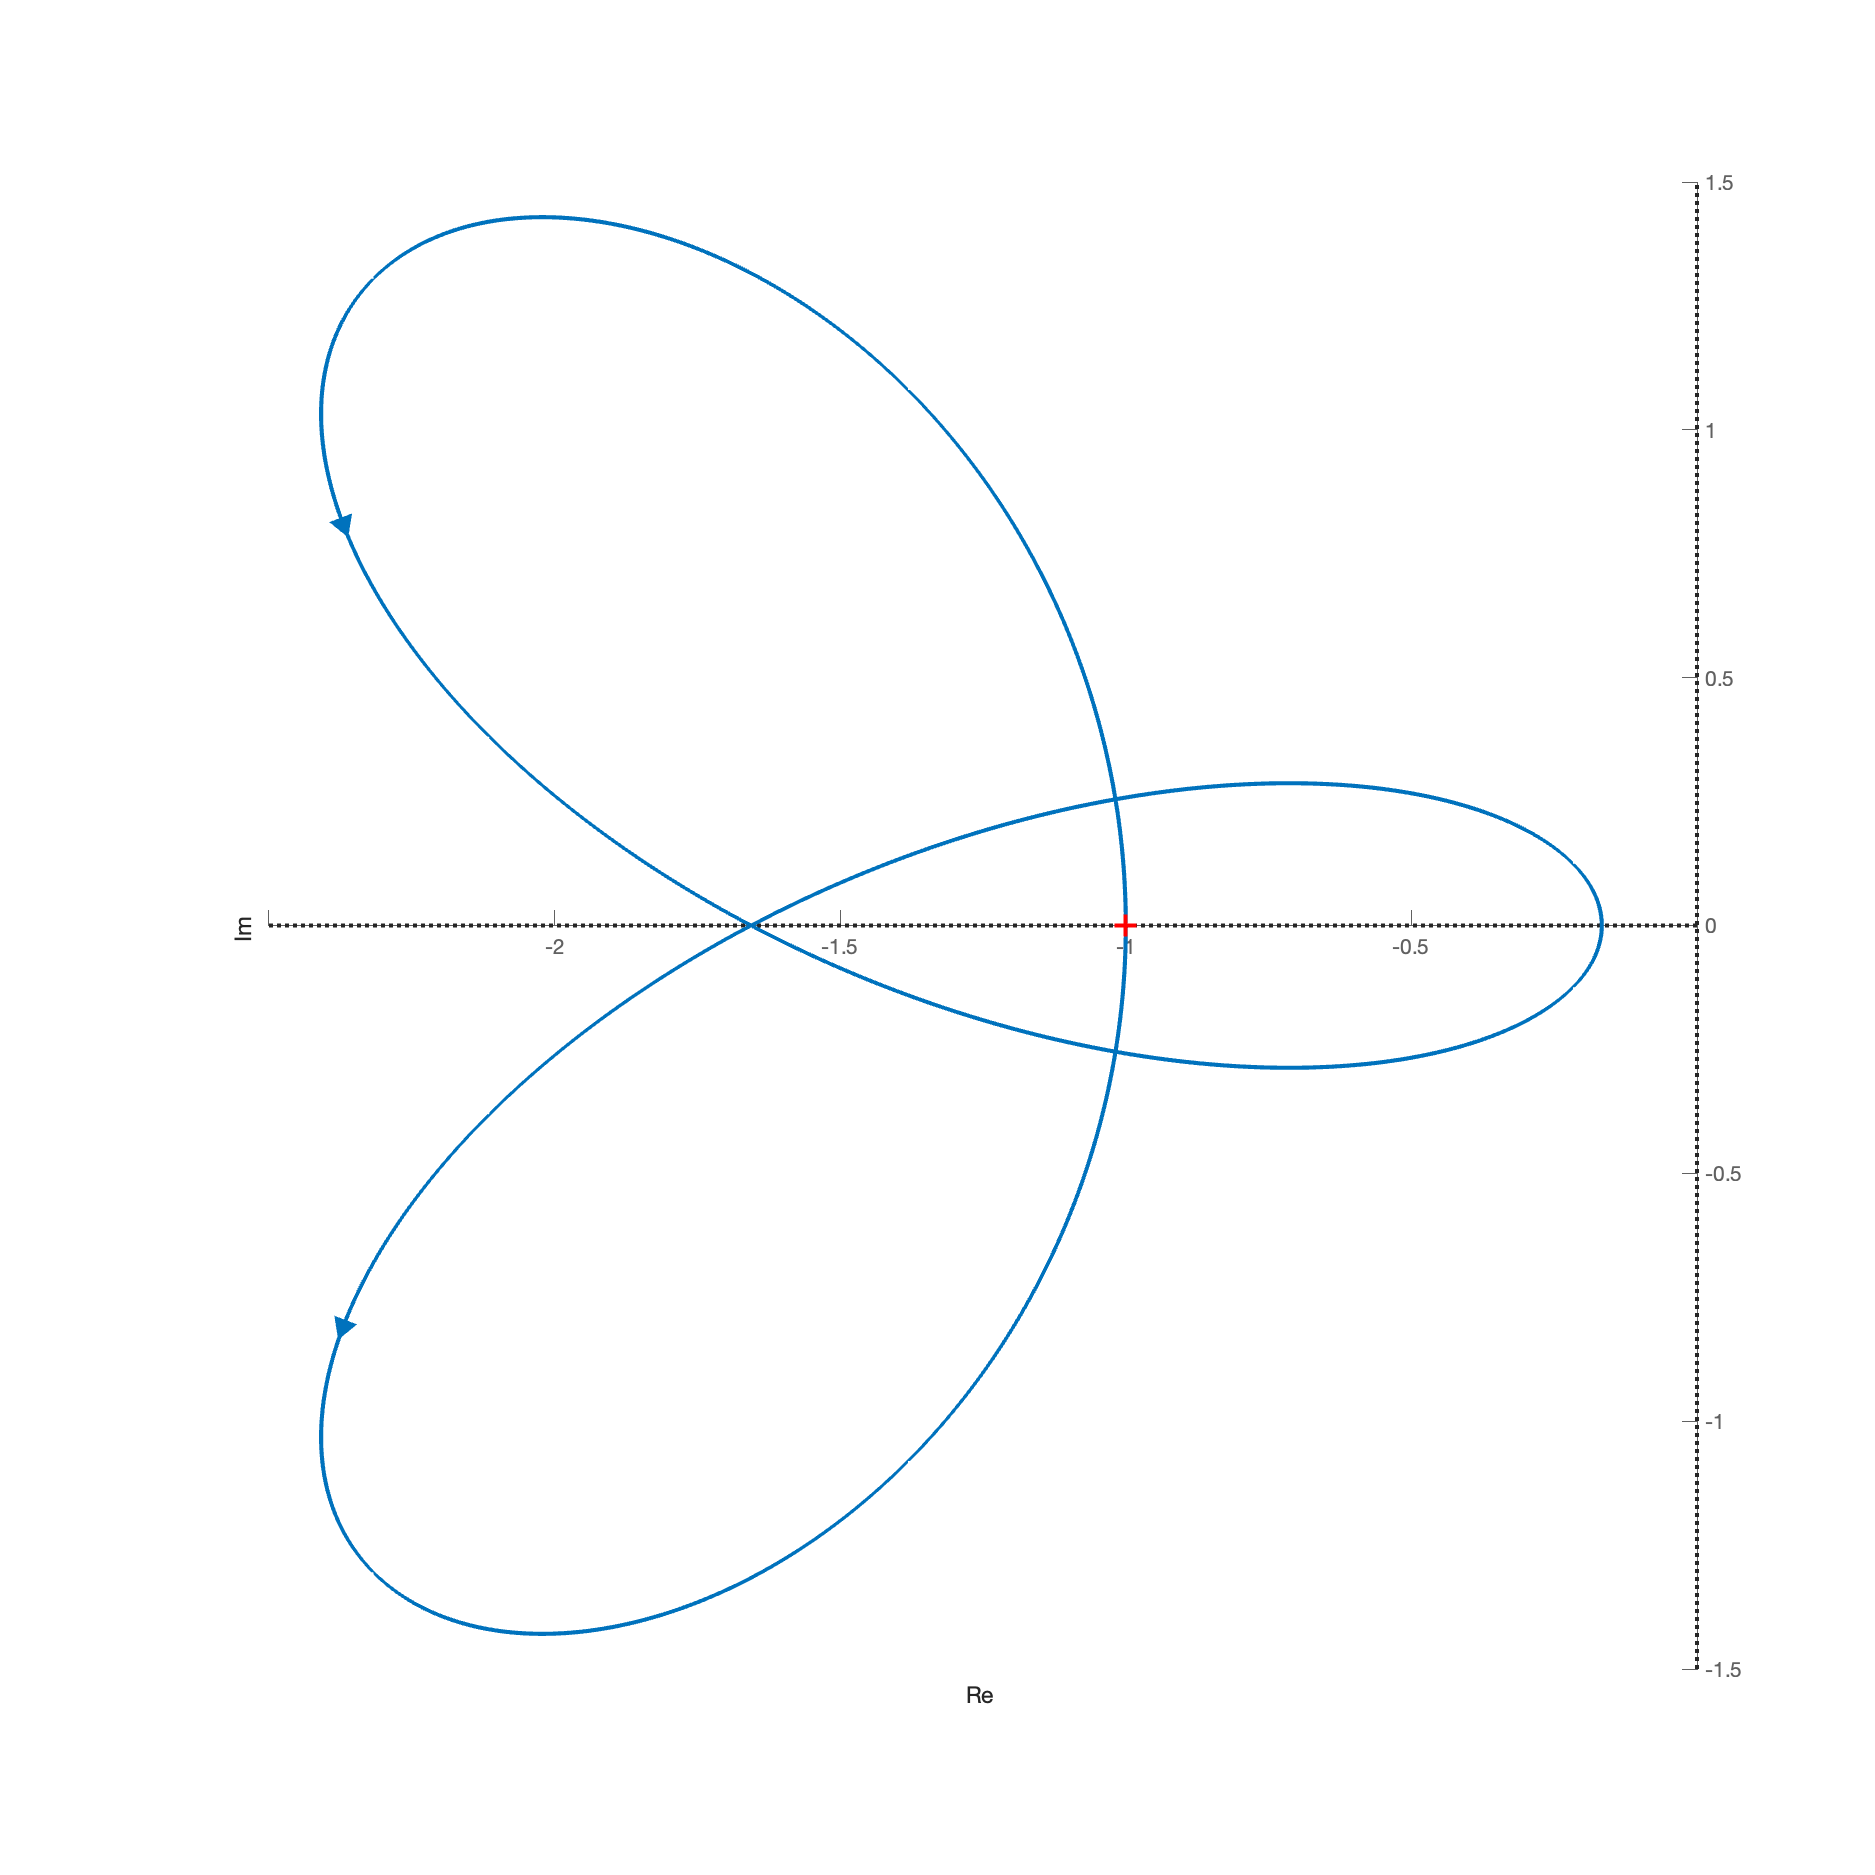
\includegraphics[width=\textwidth]{media/plots/task5_nyquist_6.png}
        \caption{$K = 1.25$}
    \end{subfigure}
    \begin{subfigure}{0.5\textwidth}
        \centering
        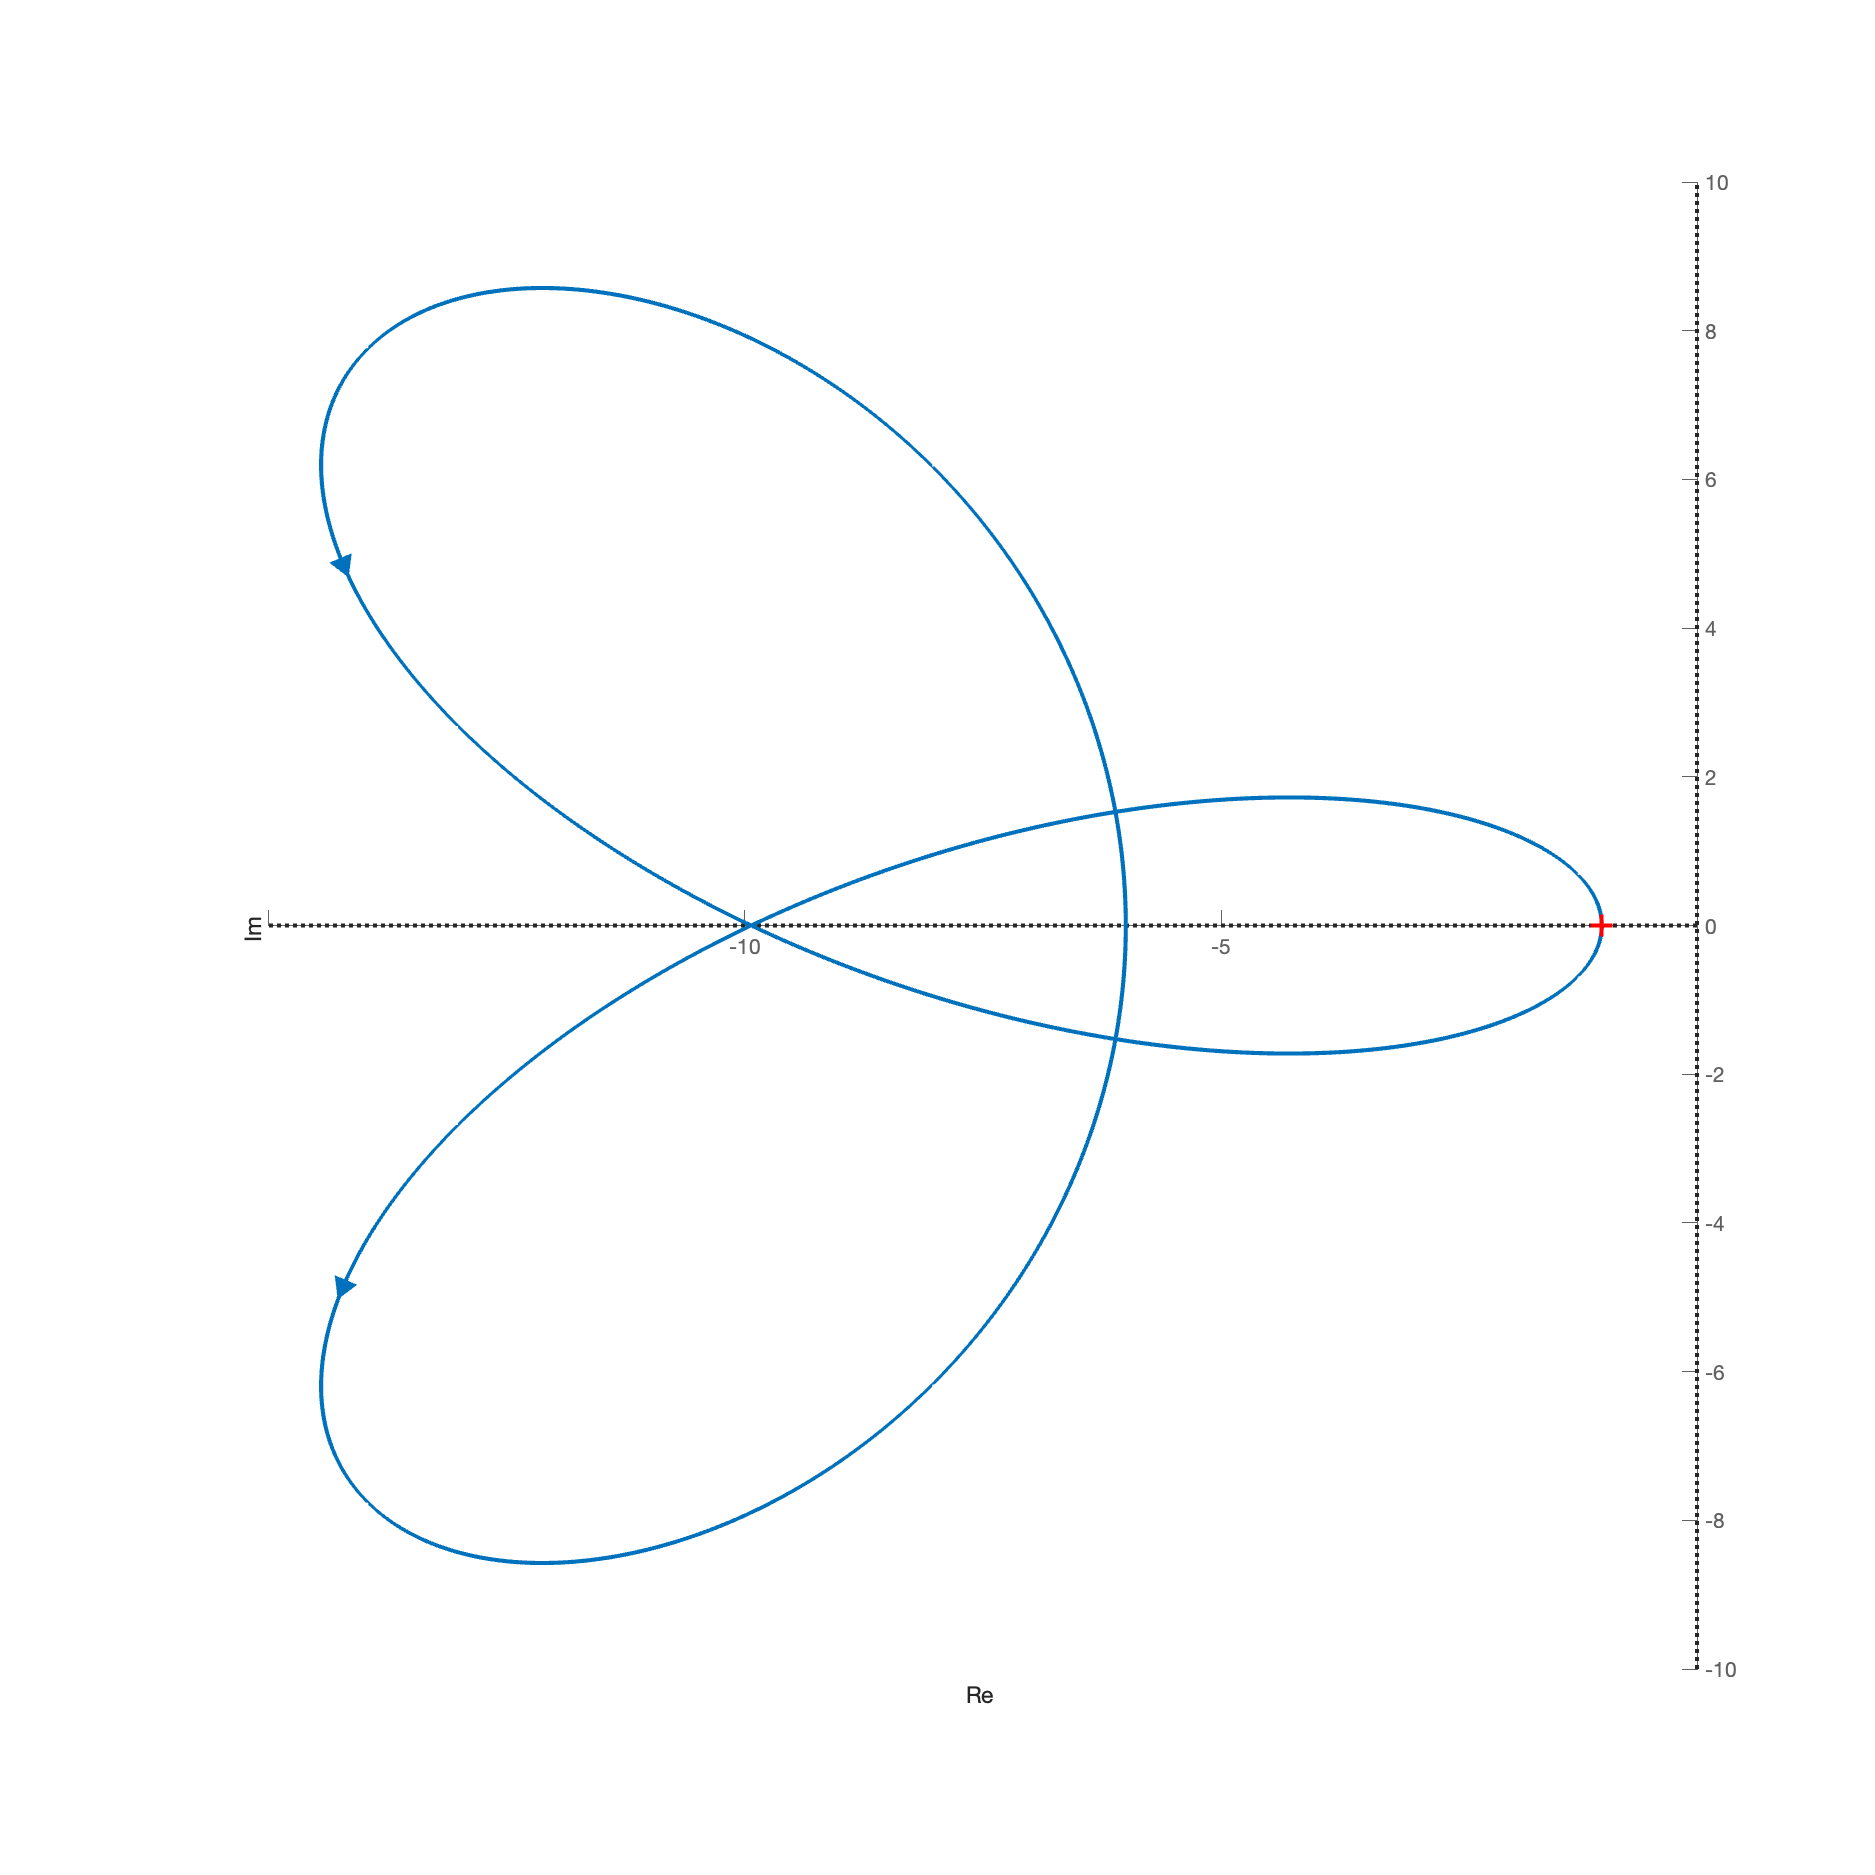
\includegraphics[width=\textwidth]{media/plots/task5_nyquist_7.png}
        \caption{$K = 7.5$}
    \end{subfigure}
    \caption{Годограф Найквиста для критических значений коэффициента усиления $K$}
    \label{fig:task5_nyquist_critical}
\end{figure}

Проведем моделирование замкнутой системы при различных значениях коэффициента усиления $K$ (см. рис. \ref{fig:task5_step} и \ref{fig:task5_impulse}).
\begin{figure}[ht!]
    \begin{subfigure}{0.5\textwidth}
        \centering
        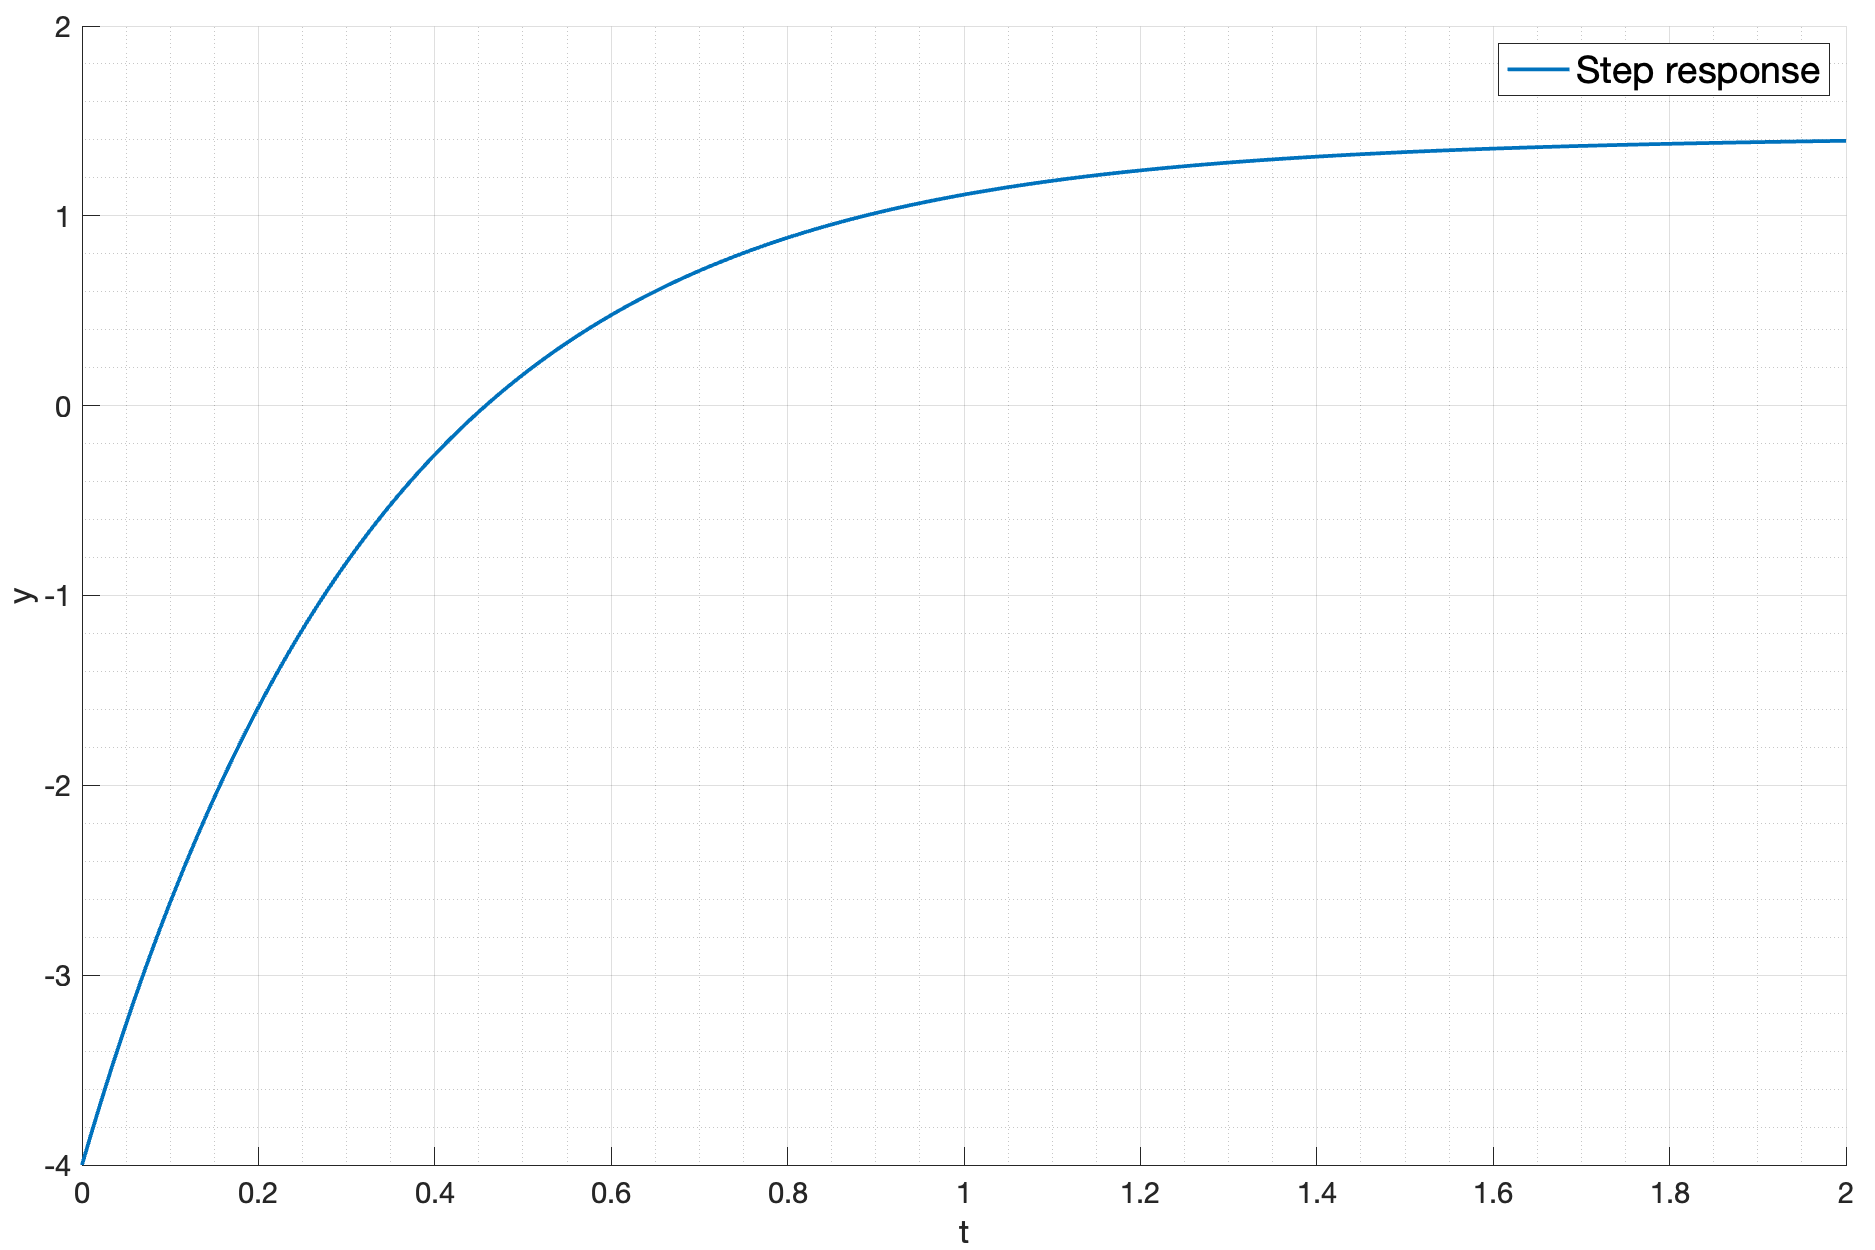
\includegraphics[width=\textwidth]{media/plots/task5_step_response_closed_1.png}
        \caption{$K = 1$}
    \end{subfigure}
    \begin{subfigure}{0.5\textwidth}
        \centering
        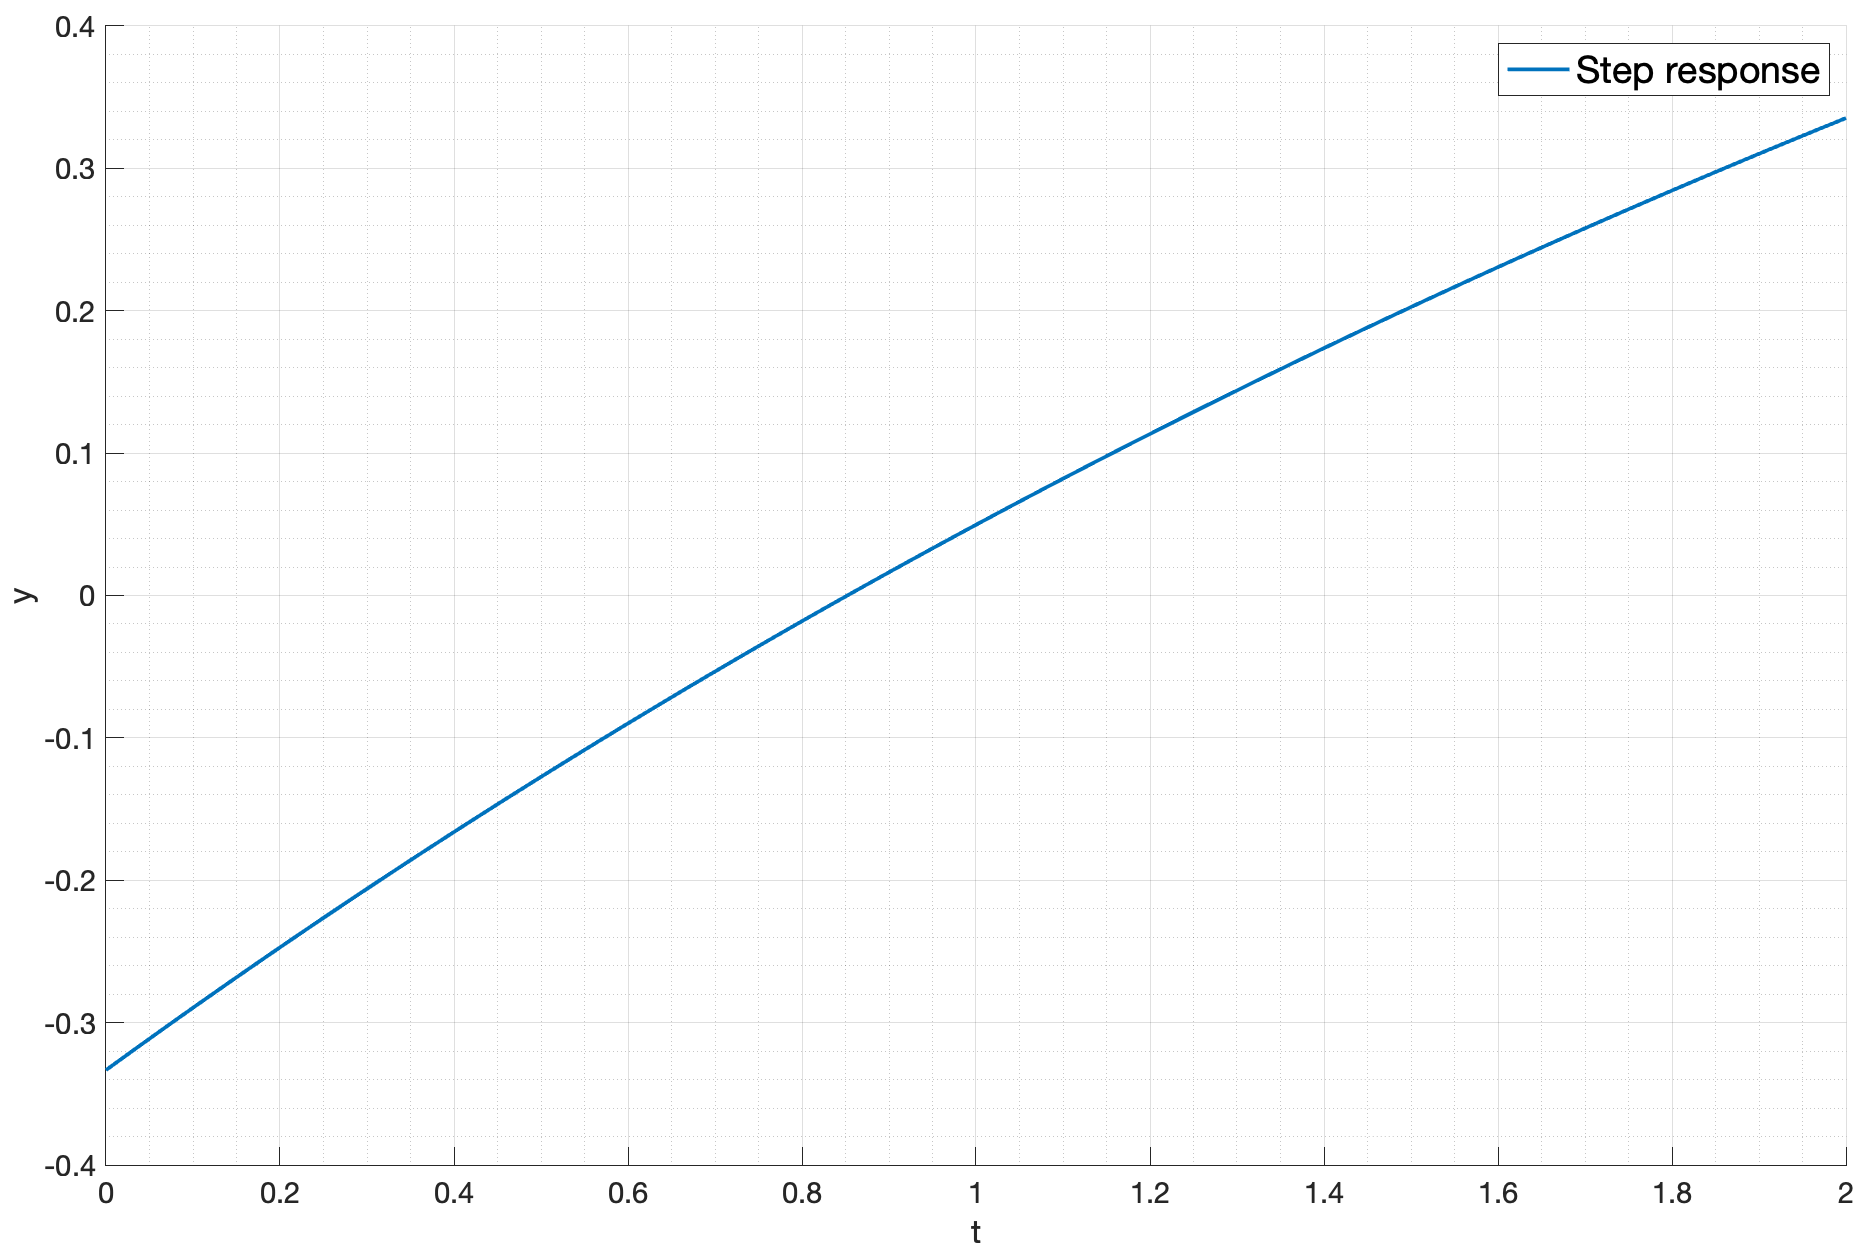
\includegraphics[width=\textwidth]{media/plots/task5_step_response_closed_2.png}
        \caption{$K = 0.5$}
    \end{subfigure}
    \begin{subfigure}{0.5\textwidth}
        \centering
        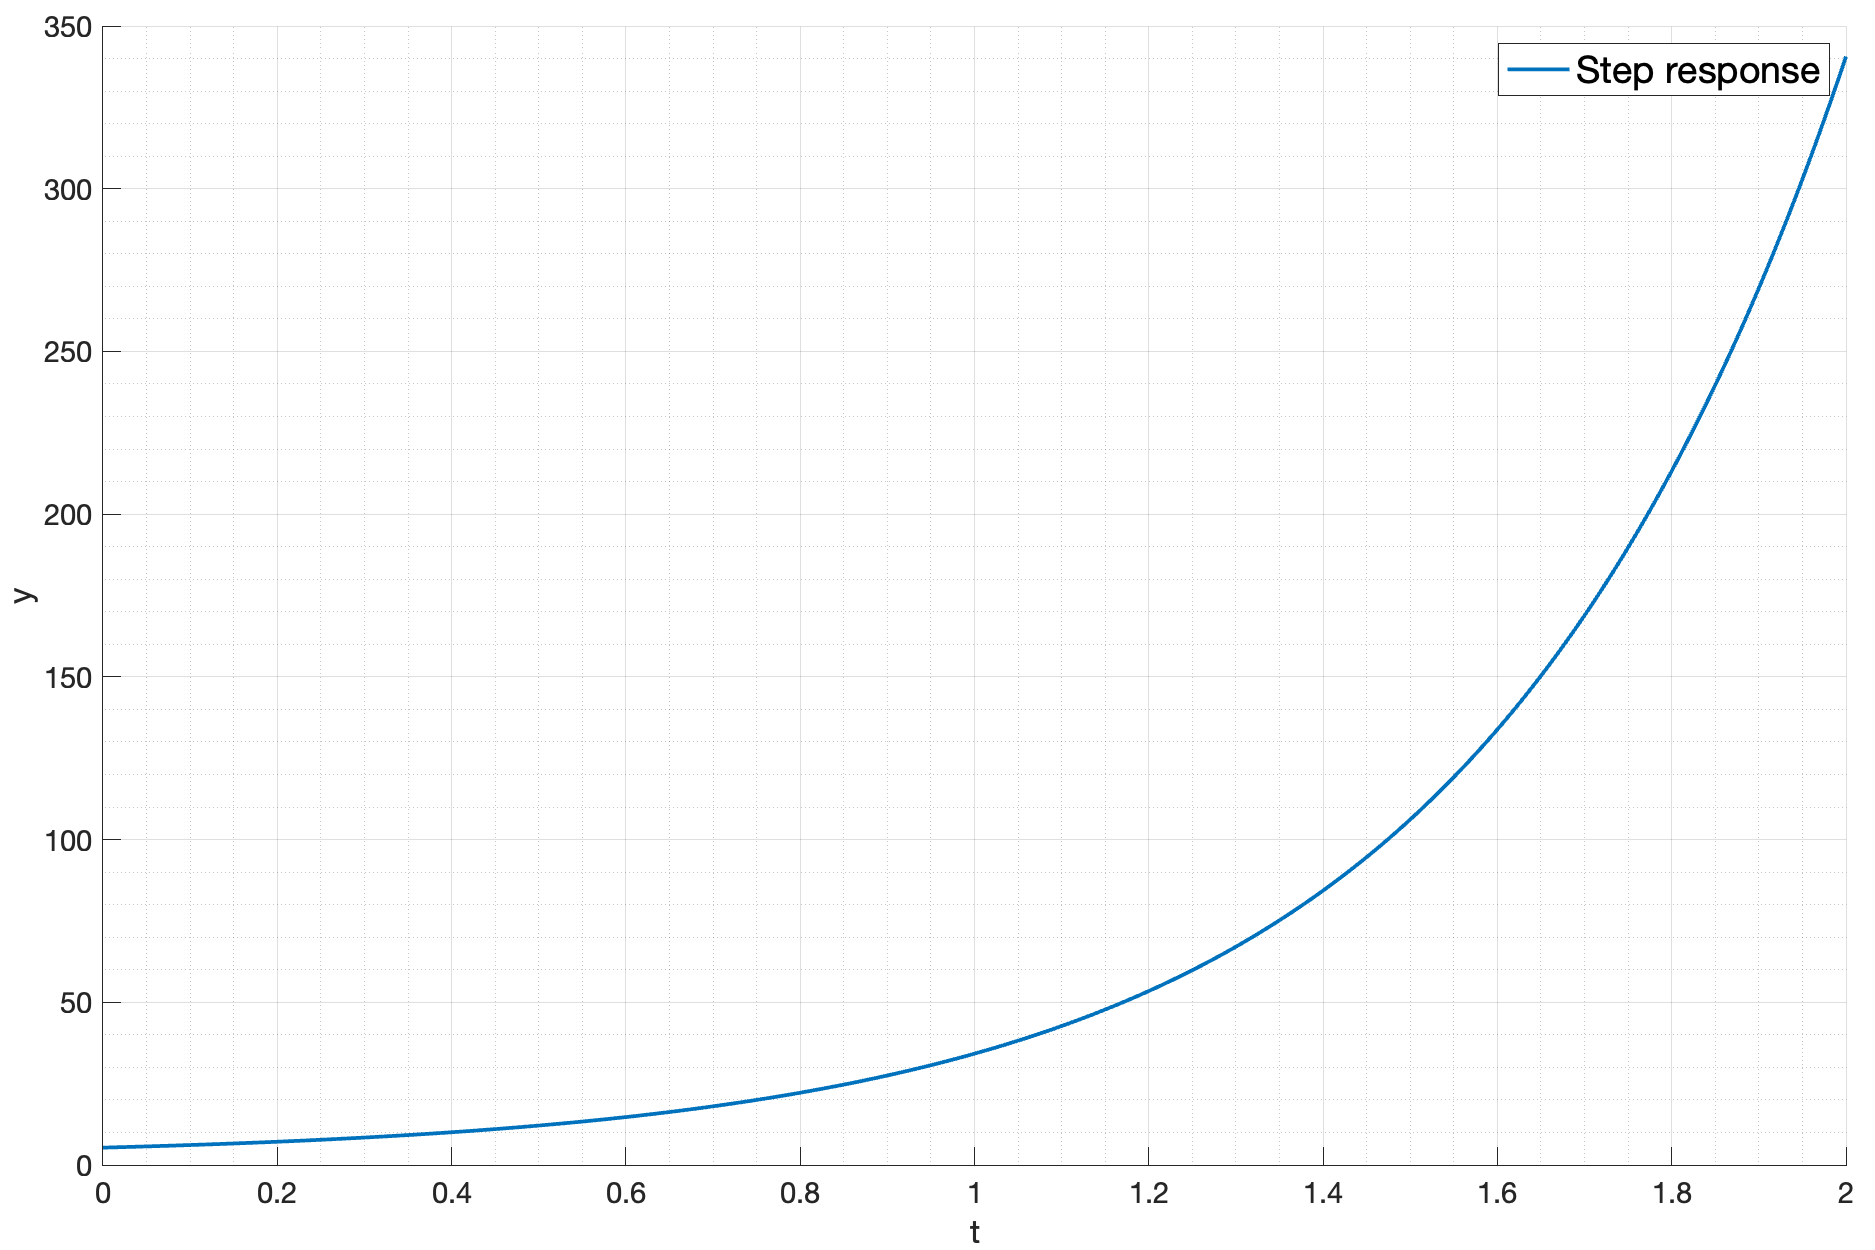
\includegraphics[width=\textwidth]{media/plots/task5_step_response_closed_3.png}
        \caption{$K = 2$}
    \end{subfigure}
    \begin{subfigure}{0.5\textwidth}
        \centering
        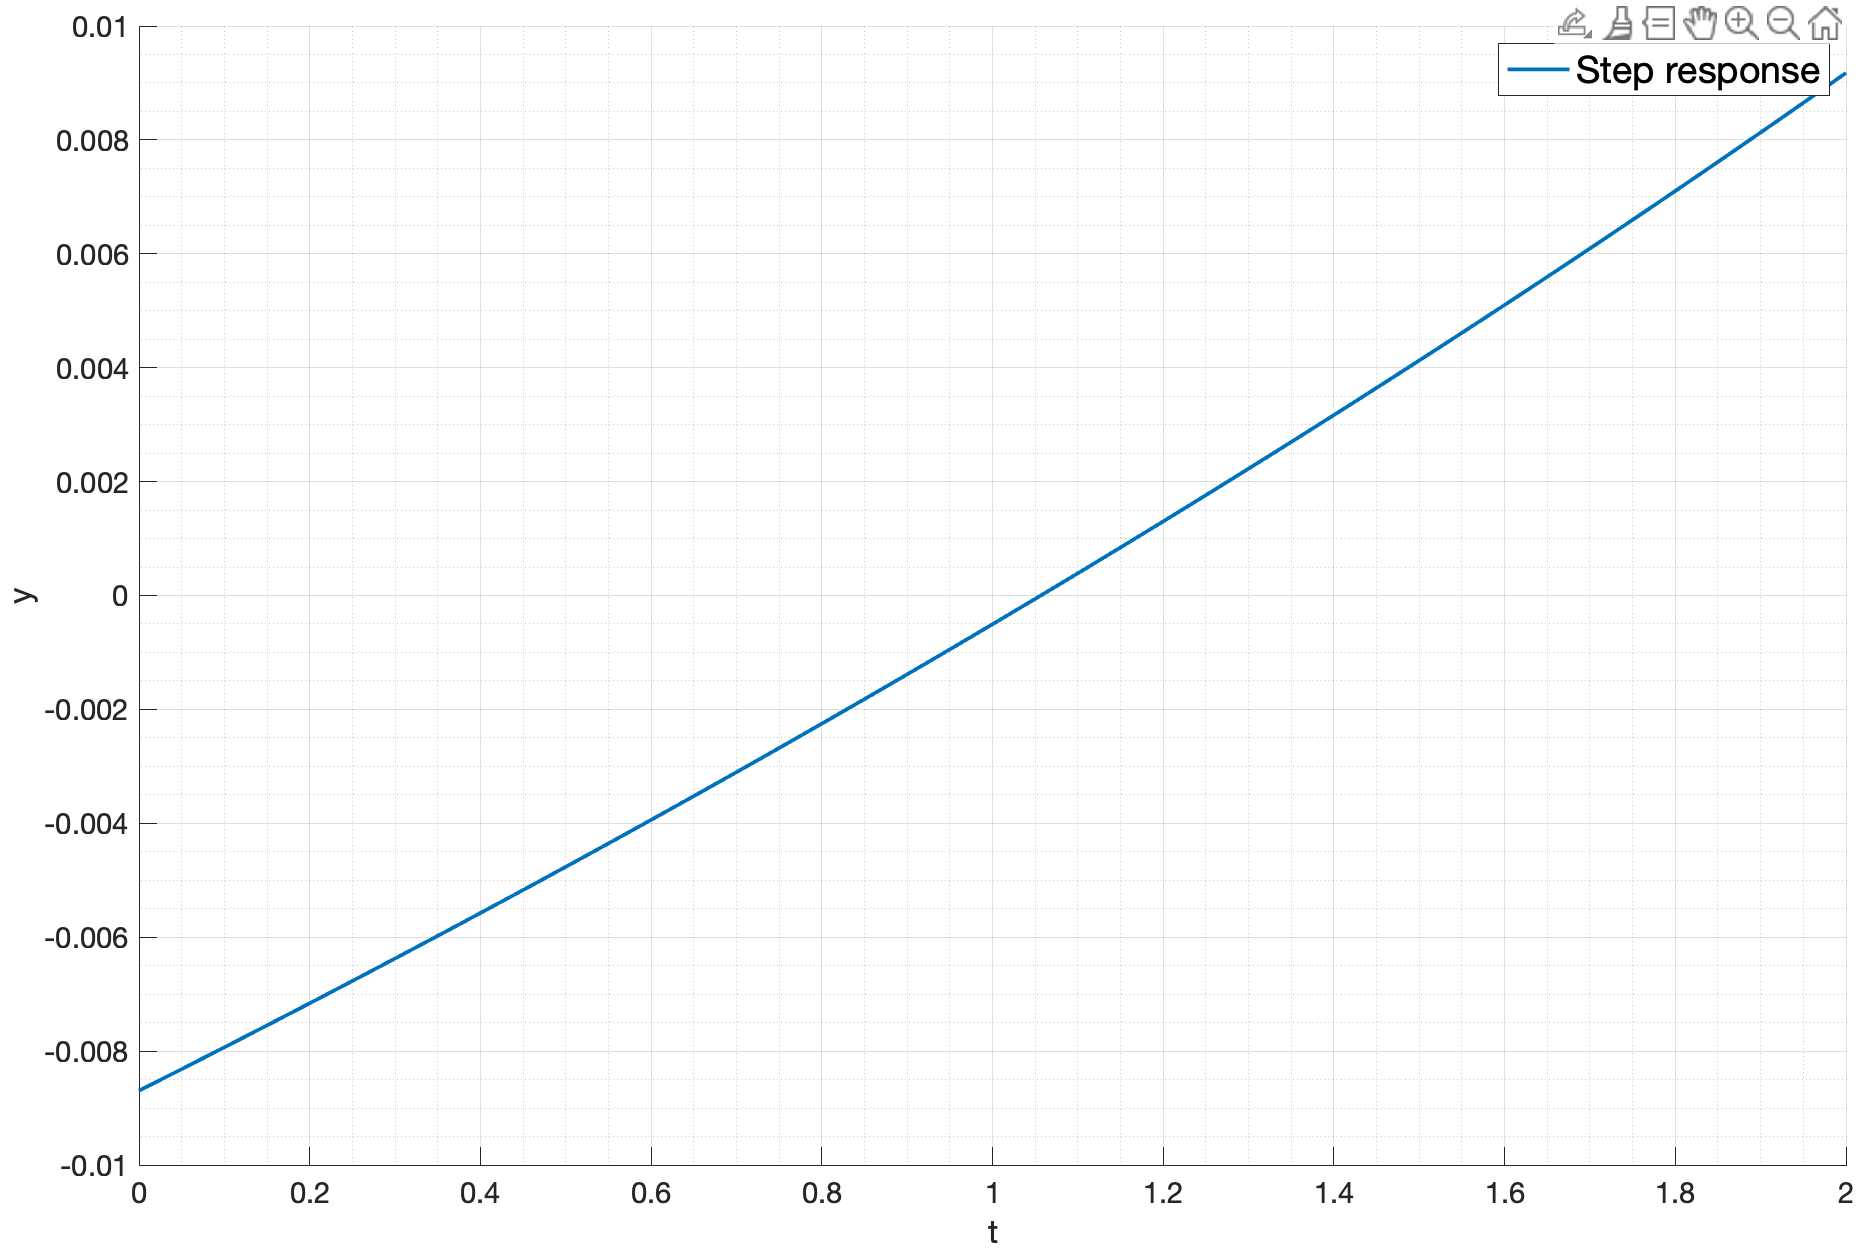
\includegraphics[width=\textwidth]{media/plots/task5_step_response_closed_4.png}
        \caption{$K = 0.1$}
    \end{subfigure}
    \caption{Переходная характеристика замкнутой системы при различных значениях коэффициента усиления $K$}
    \label{fig:task5_step}
\end{figure}

\begin{figure}[ht!]
    \begin{subfigure}{0.5\textwidth}
        \centering
        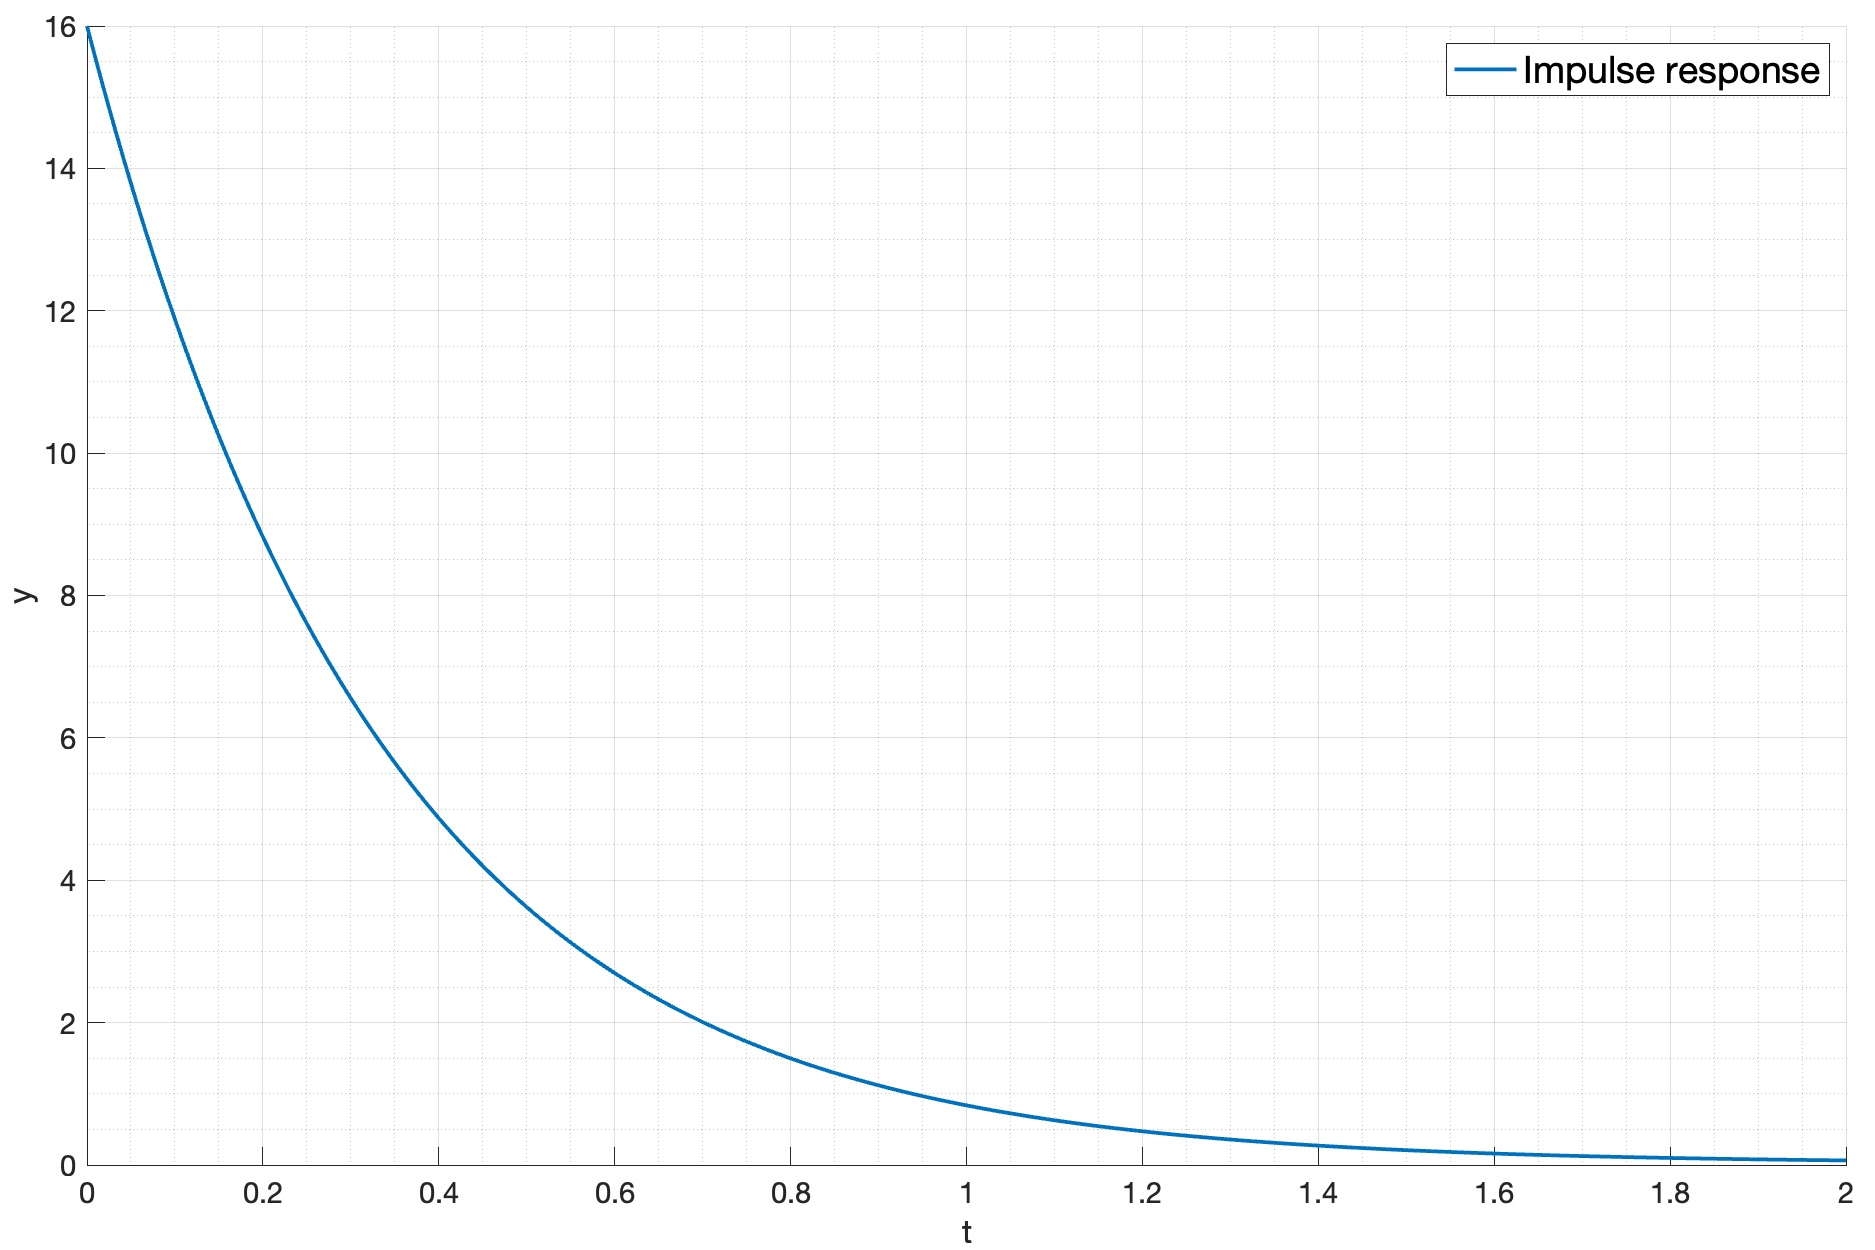
\includegraphics[width=\textwidth]{media/plots/task5_impulse_response_closed_1.png}
        \caption{$K = 1$}
    \end{subfigure}
    \begin{subfigure}{0.5\textwidth}
        \centering
        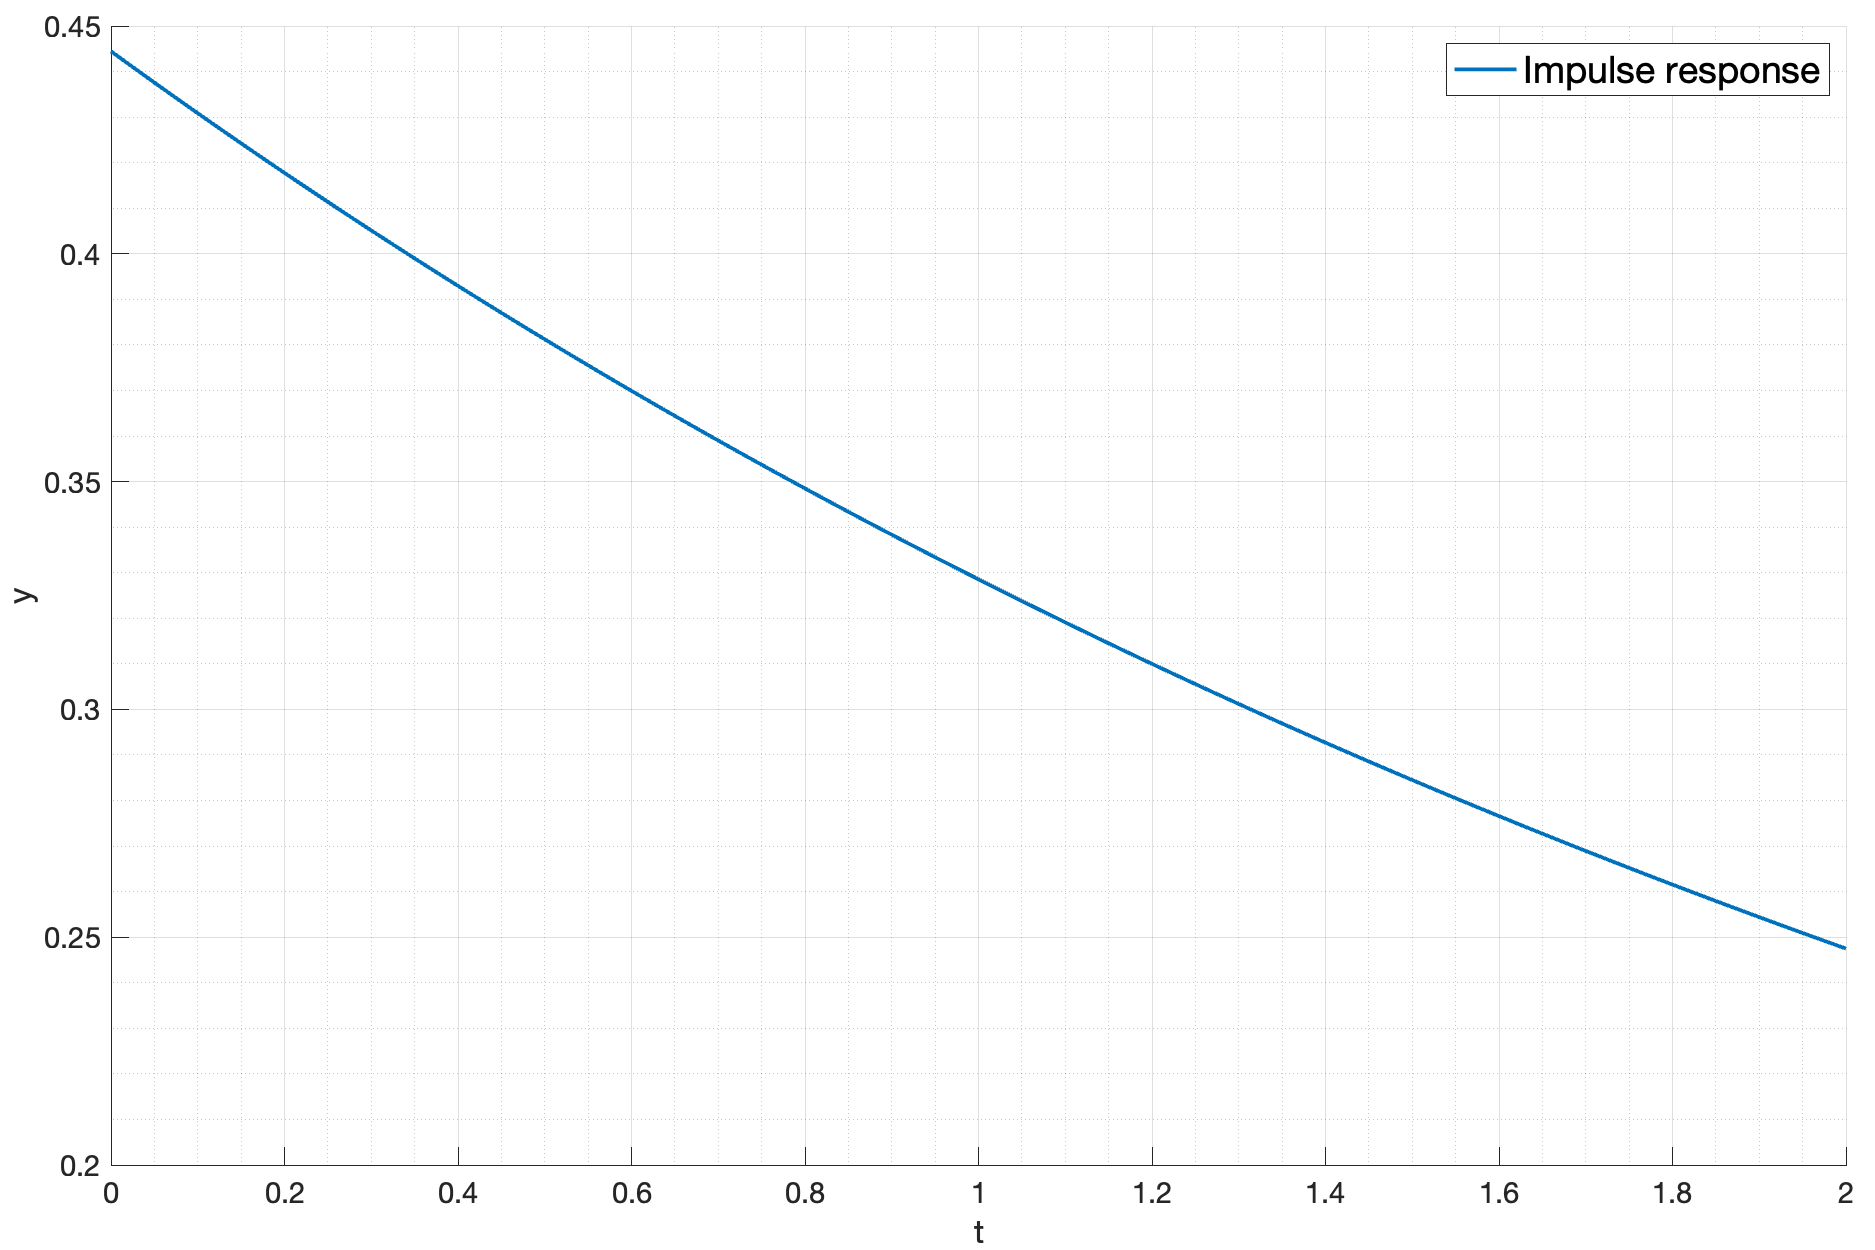
\includegraphics[width=\textwidth]{media/plots/task5_impulse_response_closed_2.png}
        \caption{$K = 0.5$}
    \end{subfigure}
    \begin{subfigure}{0.5\textwidth}
        \centering
        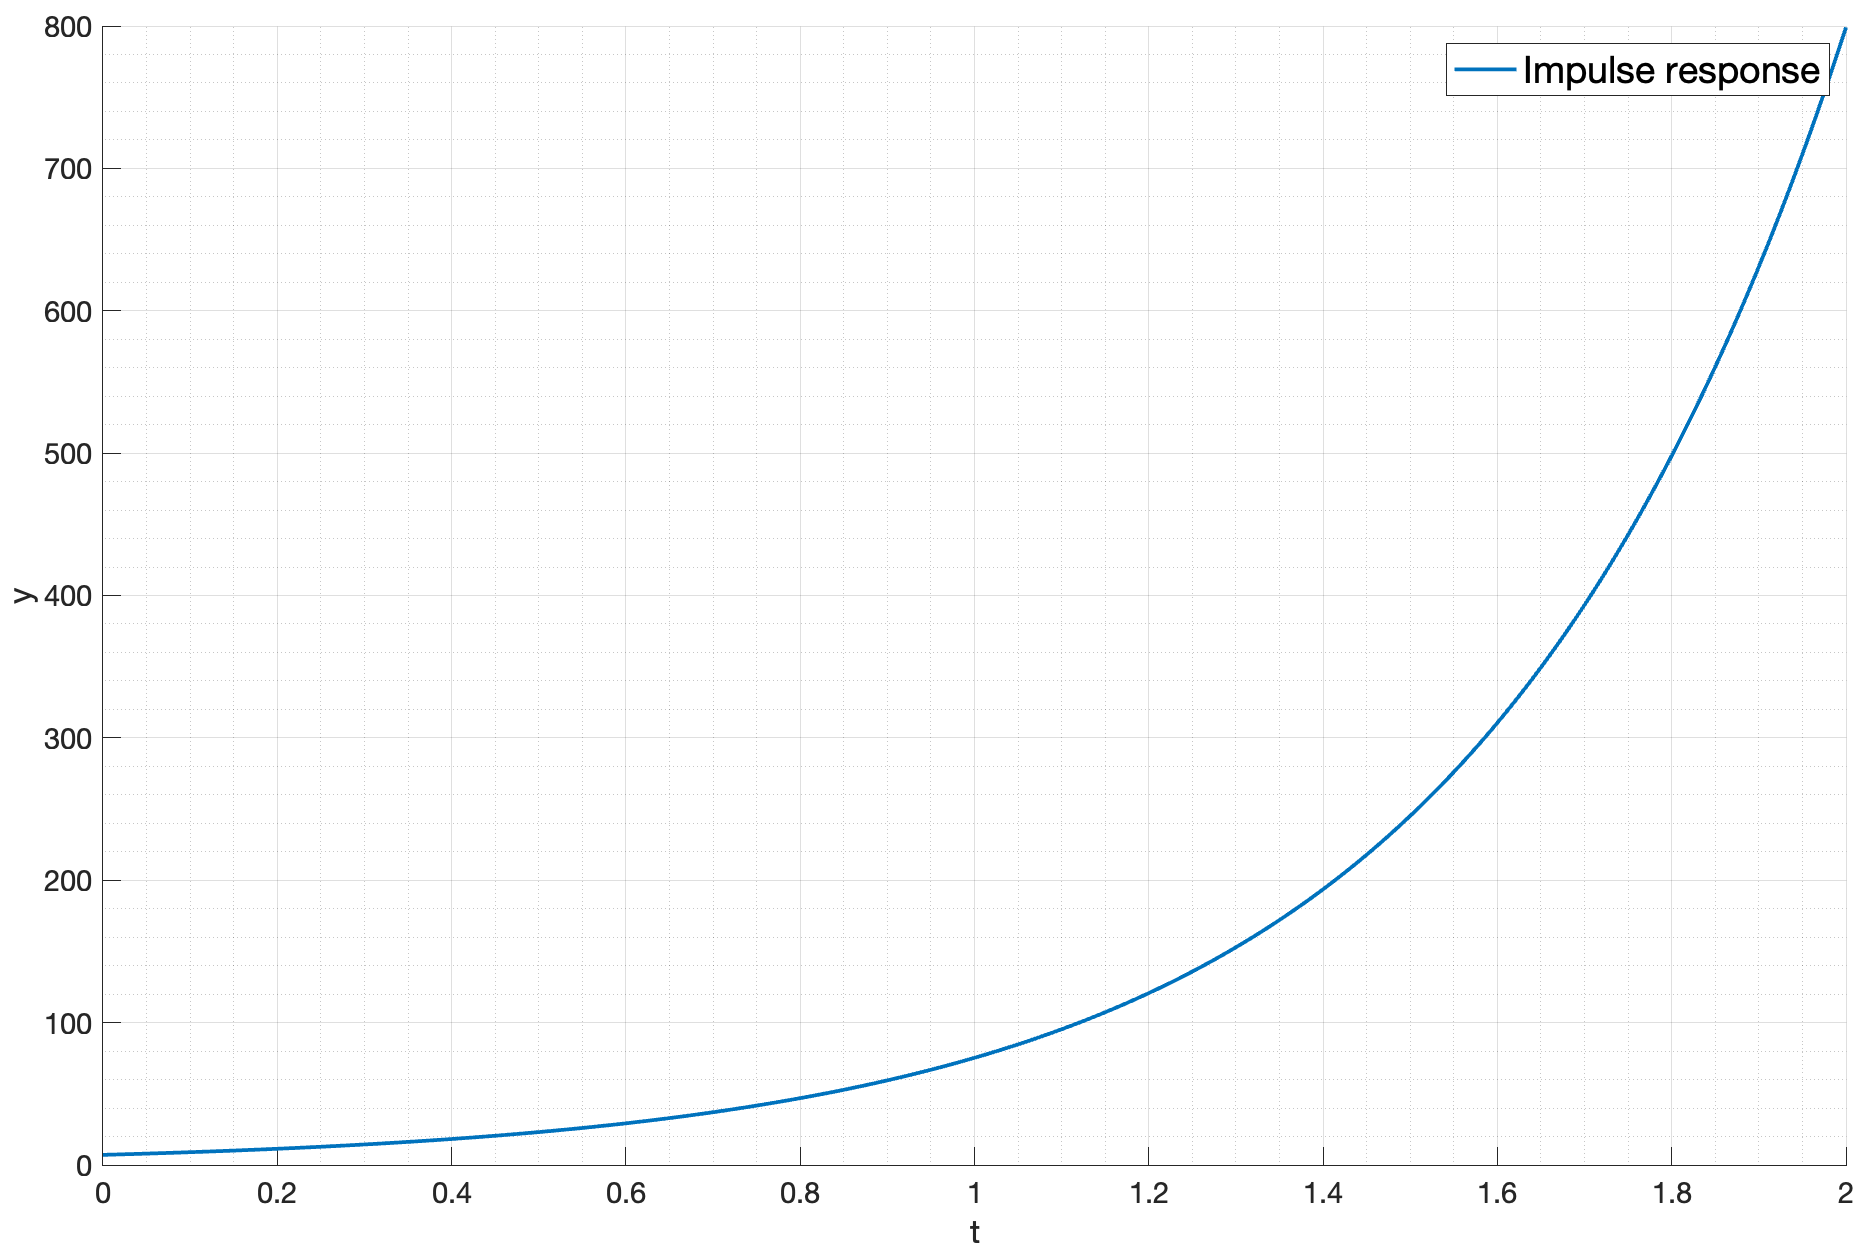
\includegraphics[width=\textwidth]{media/plots/task5_impulse_response_closed_3.png}
        \caption{$K = 2$}
    \end{subfigure}
    \begin{subfigure}{0.5\textwidth}
        \centering
        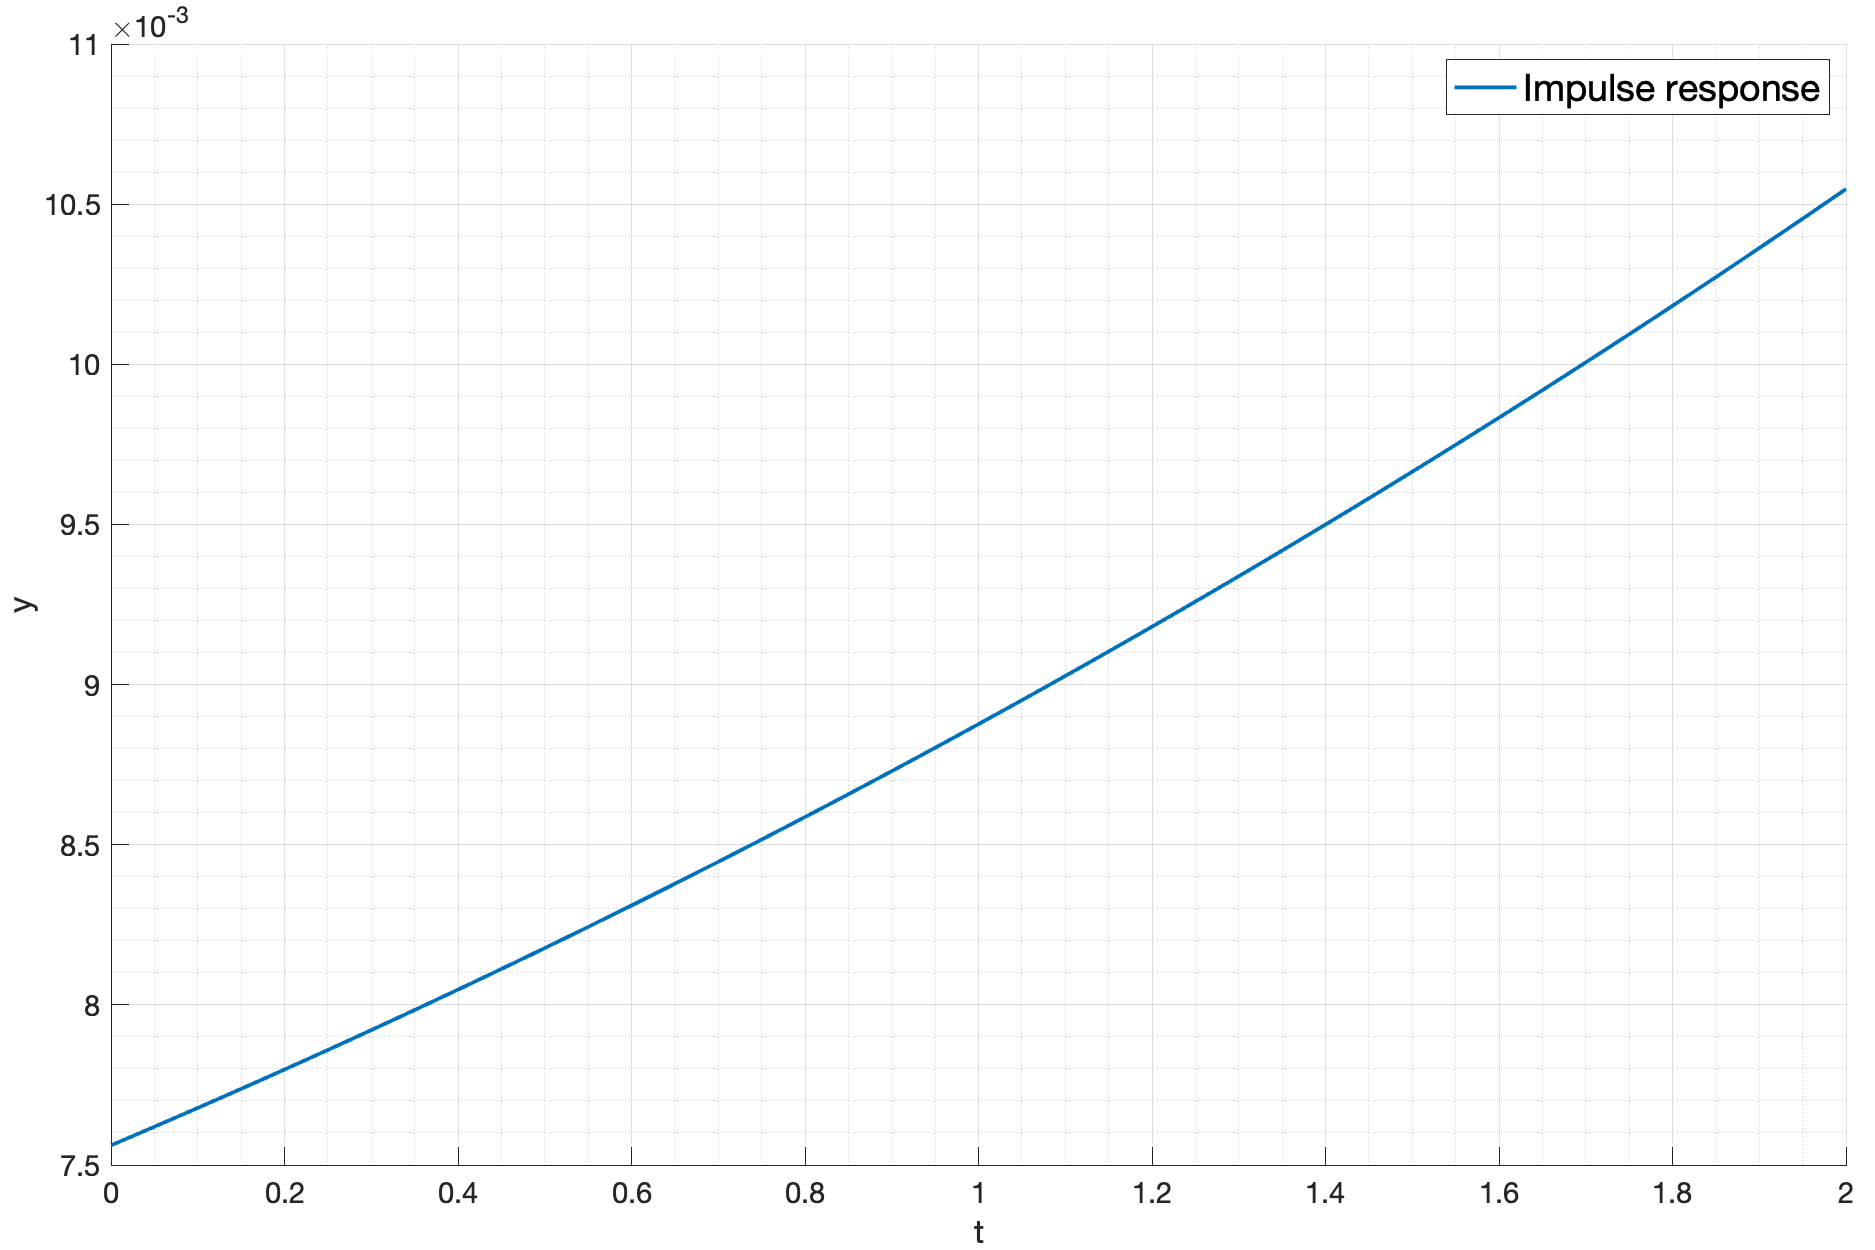
\includegraphics[width=\textwidth]{media/plots/task5_impulse_response_closed_4.png}
        \caption{$K = 0.1$}
    \end{subfigure}
    \caption{Импульсная характеристика замкнутой системы при различных значениях коэффициента усиления $K$}
    \label{fig:task5_impulse}
\end{figure}

Теоретические результаты совпадают с результатами моделирования: система устойчива при $K \in (0.75, 1.25)$,

Найдем запас устойчивости по амплитуде для системы при $K = 1$. Для этого воспользуемся 
годографом Найквиста (см. рис. \ref{fig:task5_nyquist}).
\begin{figure}[ht!]
    \centering
    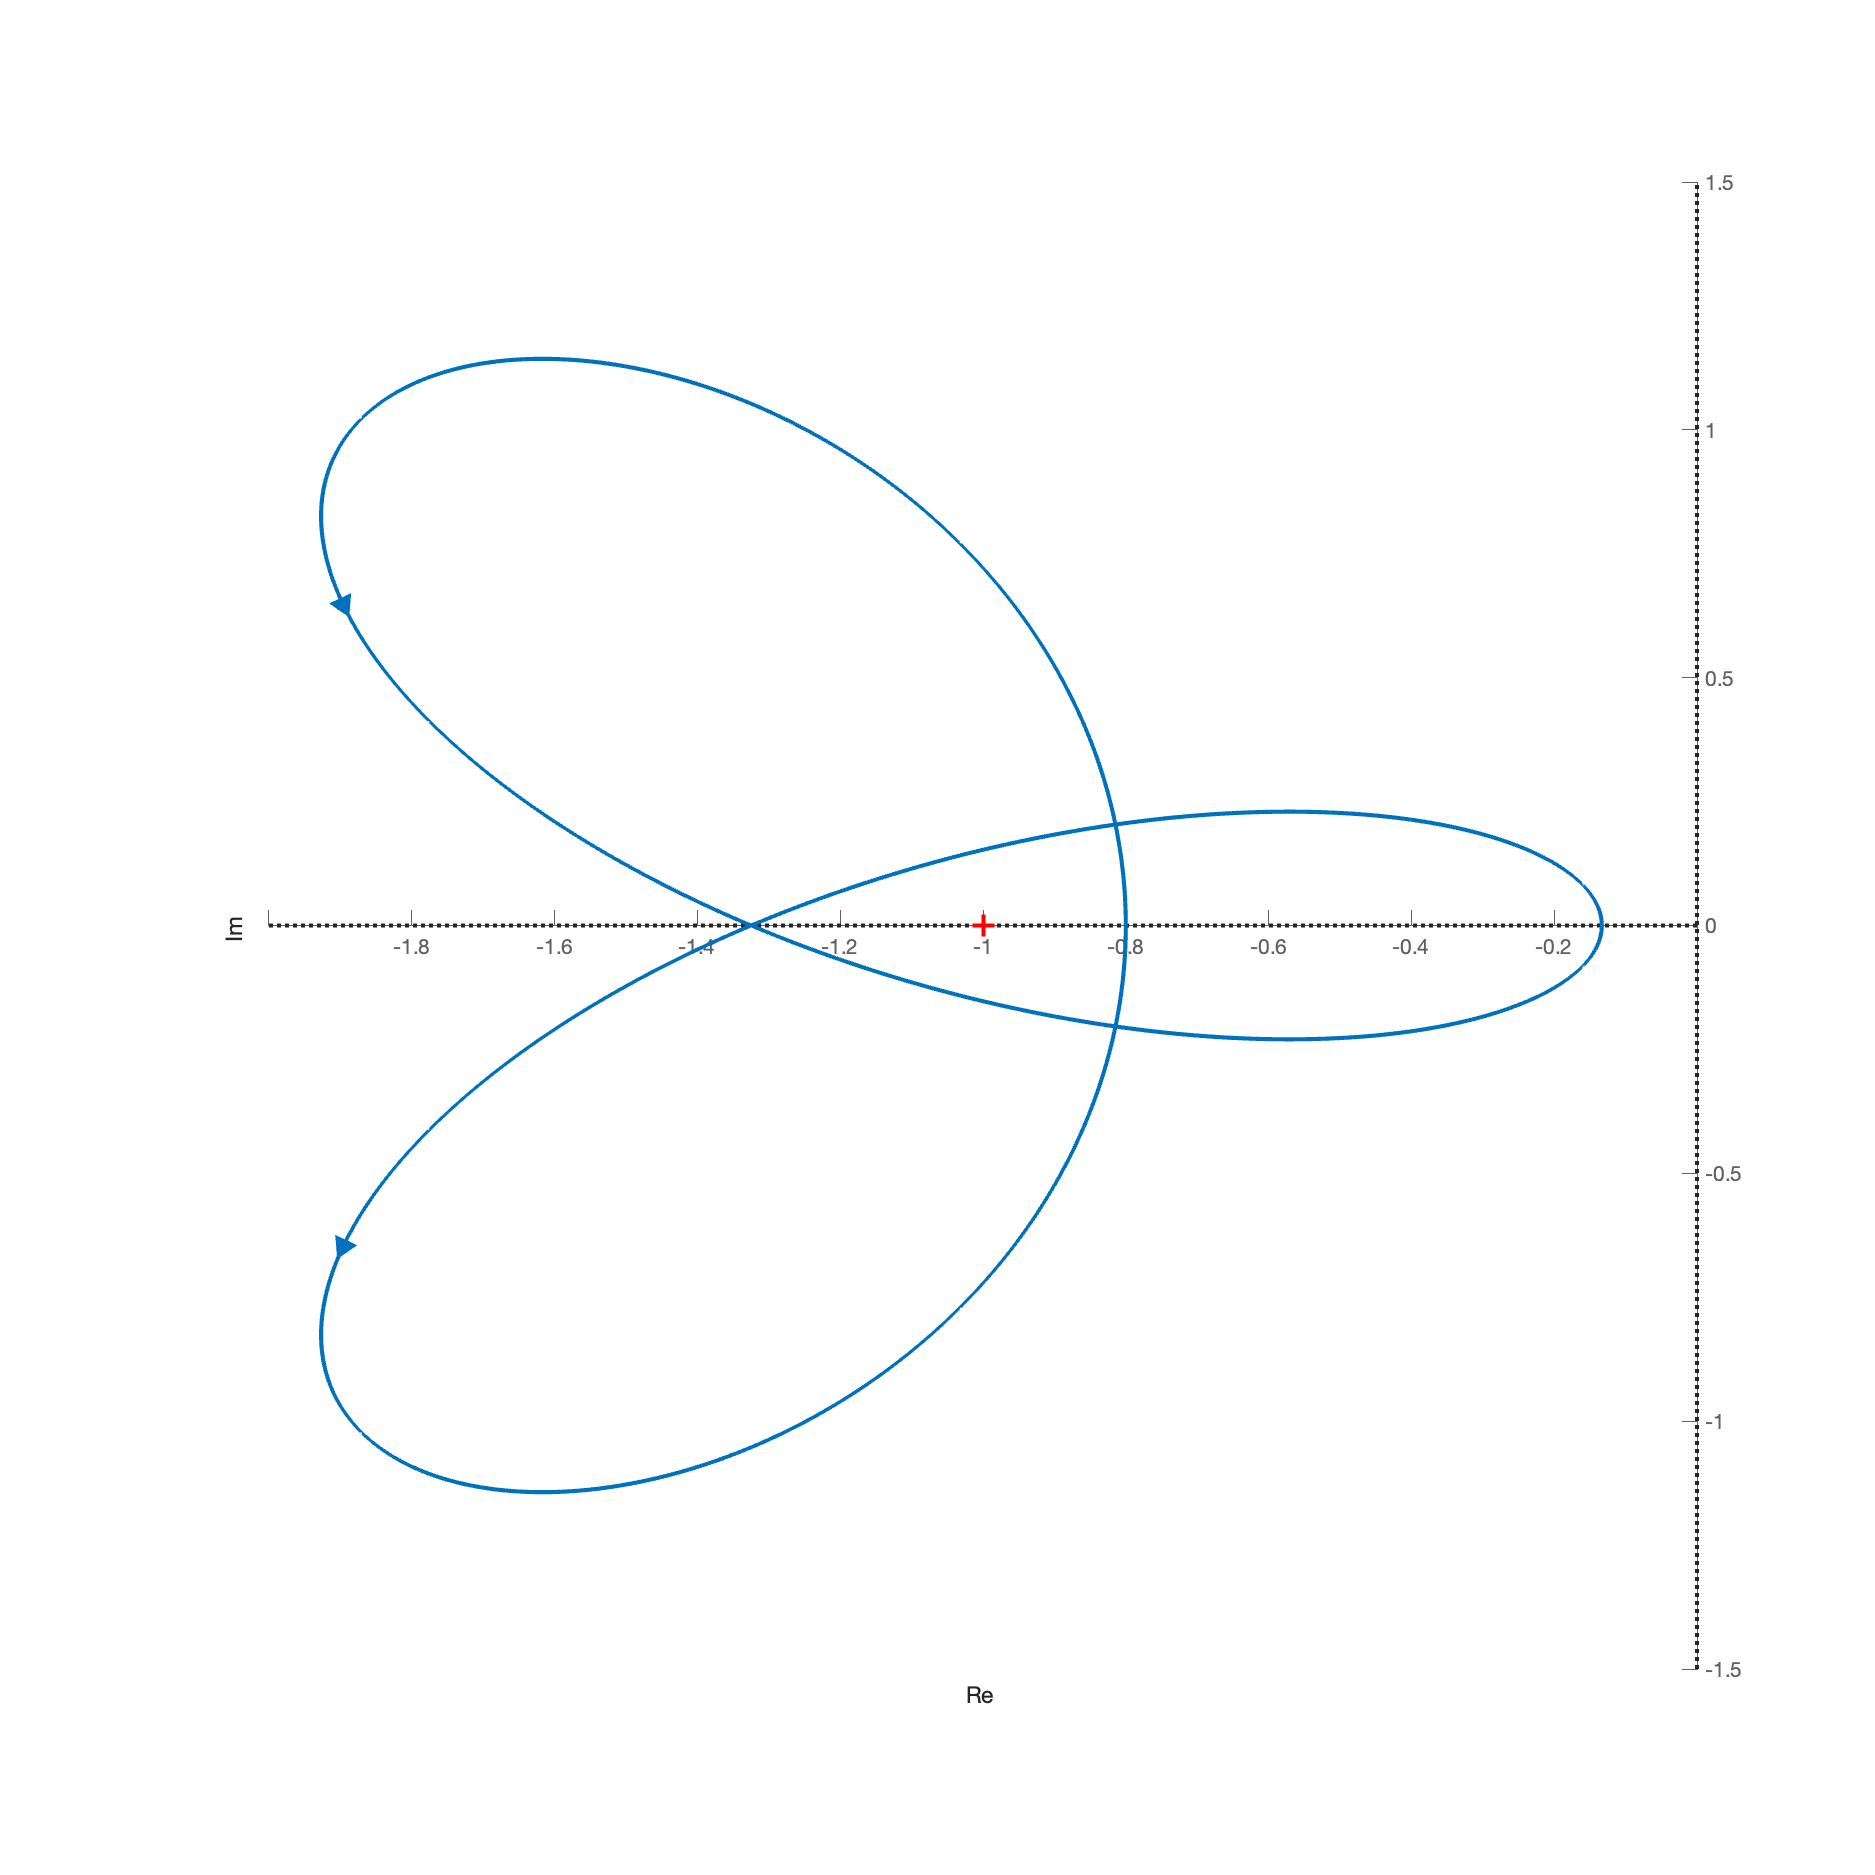
\includegraphics[width=\textwidth]{media/plots/task5_nyquist_1.png}
    \caption{Годограф Найквиста для $K = 1$}
    \label{fig:task5_nyquist}
\end{figure}
Исходя из предыдущих вычислений и симуляции, можно понять, что система будет устойчива тогда, когда 
годограф делает ровно два оборота вокруг точки $(-1, 0)$ против часовой стрелки. 
Таким образом, есть две критические зоны: 
\begin{equation}
    A_1 = 0.8 \quad A_2 \approx 1.33 
\end{equation}
Согласно этому: 
\begin{equation}
    A_{c1} = \frac{1}{A_1} = \frac{1}{0.8} = 1.25 \quad A_{c2} = \frac{1}{A_2} = \frac{1}{1.33} \approx 0.75
\end{equation}
Таким образом, запас устойчивости по амплитуде равен $1.25$. 
Что совпадает с результатами, полученными ранее.

\subsection{Вывод}
В данном разделе были рассмотрены две системы, заданные передаточными функциями.
Были построены годографы Найквиста для различных значений коэффициента усиления $K$.
Были найдены значения коэффициента усиления, при которых замкнутая система будет устойчивой с помощью 
анализа полюсов передаточной функции.
Были найдены запасы устойчивости по амплитуде для каждой системы при помощи годографа Найквиста и АФЧХ. 
Критические значения для обоих способов совпали. 